% Speed-up compilation
% cd docs/reports/final-report
% # Chạy 2 lần để cập nhật đầy đủ Mục lục (TOC), Danh sách hình/bảng và tham chiếu chéo (\Cref)
% pdflatex -interaction=nonstopmode report.tex
% pdflatex -interaction=nonstopmode report.tex
% Đổi sang {hcmut-report} nếu viết hoàn toàn bằng tiếng Anh
\documentclass[twoside,final]{hcmut-report-vi}
\usepackage{codespace}

% Encodings & Symbols
\usepackage{gensymb,textcomp}

% Better tables
\usepackage{array,longtable,multicol,multirow,siunitx,tabularx}

% Better enum
\usepackage{enumitem}

% Graphics
\usepackage{caption,float}
\usepackage[export]{adjustbox}

% References
% Use \Cref{} instead of \ref{}
\usepackage[nameinlink]{cleveref}

% ===================================================
% THÔNG TIN TRANG BÌA (COVER CONFIGURATION)
% ===================================================
\coursename{Công nghệ Phần mềm (CO3001) -- HK261}
\reporttype{Báo cáo Tổng kết Bài tập lớn}
\title{Smart E-Mobility Hub -- Hệ thống Điều phối Phương tiện Điện ĐHQG-HCM}
\advisor{Nguyễn Thành Công &}
\stuname{%
  Trần Đình Ý --  2414100 \\
  & Nguyễn Đình Minh --  2412079 \\
  & Trần Văn Minh Triết -- 2413603 \\
  & Nguyễn Thanh Duy --  2410536 \\
}

% ===================================================
% NỘI DUNG CHÍNH
% ===================================================
\begin{document}

\coverpage

% Tạo mục lục và các danh sách
\tableofcontents
\listoffigures
\listoftables
\lstlistoflistings
\pagestyle{empty}
\clearpage

% Nội dung các chương (chia theo từng file trong sections/)
\pagestyle{fancy}
\setcounter{page}{1}

% ===================================================
% MỞ ĐẦU: THÔNG TIN NHÓM, PHÂN CÔNG VÀ THUẬT NGỮ
% Nguồn: GLOSSARY.md, docs/architecture/DEVELOPMENT_GUIDE.md,
%        docs/architecture/API_CONTRACTS.md, app/src/app.js
% ===================================================
\section*{Mở đầu: Giới thiệu, Phân công và Thuật ngữ Hệ thống}
\addcontentsline{toc}{section}{Mở đầu: Giới thiệu, Phân công và Thuật ngữ Hệ thống}

Báo cáo này trình bày quá trình phân tích yêu cầu, thiết kế hệ thống, hiện thực sản phẩm khả dụng tối thiểu (MVP) và kiểm thử cho đề tài \textbf{Smart E-Mobility Hub -- Hệ thống Điều phối Phương tiện Điện ĐHQG-HCM} trong học phần \textit{Công nghệ Phần mềm (CO3001 -- HK261)}. Nội dung báo cáo được tổ chức thành sáu chương bám sát các cột mốc của học phần: đặc tả yêu cầu và Use Case (Chương~1), mô hình động và thiết kế giao diện (Chương~2), kiến trúc 4+1 View, mô hình lớp và cơ sở dữ liệu (Chương~3), hiện thực MVP, kiểm thử và trình diễn (Chương~4), đánh giá kết quả và bài học kinh nghiệm (Chương~5), cùng khai báo sử dụng Generative AI và quản trị nhóm (Chương~6).

Về phạm vi kỹ thuật, phiên bản MVP sử dụng kiến trúc \textit{Modular Monolith} trên nền Node.js, Express và SQLite với ba phân hệ nghiệp vụ độc lập (\textit{Operations}, \textit{Mobility \& Simulation}, \textit{Parking \& Charging}). Các thao tác tương tác phần cứng hiện được mô phỏng thông qua bộ điều hợp giả lập trong tiến trình máy chủ; các giới hạn về phạm vi tính năng và những phần mới hoàn thiện ở mức dịch vụ được ghi nhận minh bạch tại các chương thiết kế, hiện thực và đánh giá.

\subsection*{Phân công Trách nhiệm Thành viên}

Nhóm triển khai song song theo bốn phân hệ độc lập, thống nhất giao tiếp qua hợp đồng REST API và giao diện nội bộ giữa các module. \Cref{tab:team-ownership} tóm tắt phạm vi phụ trách của từng thành viên.

\begin{table}[H]
\centering\small
\caption{Phân công trách nhiệm và tỷ lệ đóng góp của các thành viên}
\label{tab:team-ownership}
\begin{tabularx}{\textwidth}{>{\raggedright\arraybackslash}p{2.5cm} >{\raggedright\arraybackslash}p{2.6cm} >{\raggedright\arraybackslash}X >{\centering\arraybackslash}p{1.6cm}}
\toprule
\textbf{Phân hệ} & \textbf{Phụ trách (MSSV)} & \textbf{Phạm vi công việc chính} & \textbf{Đóng góp} \\
\midrule
Thiết kế UX/UI & Trần Đình Ý (2414100) & Thiết kế bộ 26 màn hình bản mẫu cho User Mobile, Operator Mobile và Operator Web Dashboard cùng luồng chuyển màn hình. & \textit{[Chờ XN]} \\
\addlinespace[4pt]
Thuê xe \& Mô phỏng & Nguyễn Đình Minh (2412079) & Hiện thực luồng tìm Hub, thuê/trả xe (\texttt{UC01--UC05}), mô phỏng \textit{What-if} (\texttt{UC13--UC14}), giao diện Live Dashboard và ứng dụng khách Android/Flutter. & \textit{[Chờ XN]} \\
\addlinespace[4pt]
Đỗ xe \& Sạc điện & Trần Văn Minh Triết (2413603) & Hiện thực luồng đỗ xe cá nhân (\texttt{UC06}), yêu cầu/dừng sạc (\texttt{UC07}, \texttt{UC07A}), lập lịch sạc (\texttt{UC12}) và lược đồ dữ liệu đỗ--sạc. & \textit{[Chờ XN]} \\
\addlinespace[4pt]
Vận hành Hub & Nguyễn Thanh Duy (2410536) & Hiện thực giám sát mạng Hub, quản trị tài nguyên, điều chuyển xe và xử lý sự cố (\texttt{UC08--UC11A}), cùng tầng truy cập SQLite dùng chung. & \textit{[Chờ XN]} \\
\bottomrule
\end{tabularx}
\end{table}

\subsection*{Bảng Thuật ngữ và Ký hiệu Chuyên ngành}

\Cref{tab:glossary} chuẩn hóa các thuật ngữ miền nghiệp vụ và kỹ thuật được sử dụng xuyên suốt báo cáo.

\begin{table}[H]
\centering\small
\caption{Thuật ngữ chuyên ngành và khái niệm miền nghiệp vụ cốt lõi}
\label{tab:glossary}
\begin{tabularx}{\textwidth}{>{\raggedright\arraybackslash}p{4.2cm} >{\raggedright\arraybackslash}X}
\toprule
\textbf{Thuật ngữ / Ký hiệu} & \textbf{Định nghĩa chuẩn hóa trong hệ thống} \\
\midrule
\textbf{User / Student} & Người dùng cuối (điển hình là sinh viên) tìm kiếm Hub, đặt, nhận/trả xe dùng chung, đặt chỗ đỗ và gửi yêu cầu sạc cho xe cá nhân. \\
\addlinespace[3pt]
\textbf{Operator} & Nhân viên vận hành giám sát mạng lưới Hub, quản trị tài nguyên, điều chuyển xe, xử lý sự cố, điều phối lịch sạc và chạy mô phỏng. \\
\addlinespace[3pt]
\textbf{Mobility Hub} & Trạm trung chuyển tại ĐHQG-HCM (Ga Metro ĐHQG, Ký túc xá khu A, ĐH Bách khoa -- Cơ sở 2, Thư viện Trung tâm), tích hợp xe dùng chung, chỗ đỗ và trụ sạc. \\
\addlinespace[3pt]
\textbf{Xe dùng chung / Xe cá nhân} & Phân loại quyền sở hữu phương tiện điện: xe dùng chung (\textit{Shared}) phục vụ cho thuê và điều chuyển; xe cá nhân (\textit{Private}) chỉ sử dụng dịch vụ đỗ và sạc. \\
\addlinespace[3pt]
\textbf{Cam kết đặt chỗ và Chiếm dụng vật lý} & Phân biệt giữa \textit{cam kết đặt chỗ} (phiếu \texttt{Reserved} theo hạn giữ hoặc khung giờ hẹn) với \textit{chiếm dụng vật lý} (bản ghi thực tế chỉ phát sinh sau khi check-in tại bãi). \\
\addlinespace[3pt]
\textbf{Phân bổ sạc và Phiên sạc} & Phân biệt giữa \textit{phân bổ cổng và công suất} (trạng thái \texttt{Reserved}) với \textit{phiên sạc thực tế} (trạng thái \texttt{Active}) chỉ bắt đầu sau khi thiết bị xác nhận cấp điện. \\
\addlinespace[3pt]
\textbf{Single-Winner Semantics} & Cơ chế bảo đảm chỉ một giao dịch thành công khi nhiều yêu cầu cùng tranh chấp một xe hoặc một chỗ đỗ thông qua khóa ghi nguyên tử trong cơ sở dữ liệu. \\
\addlinespace[3pt]
\textbf{Idempotency-Key} & Khóa định danh chống lặp gắn kèm các yêu cầu ghi HTTP, giúp phát lại kết quả an toàn khi mạng chập chờn mà không tạo giao dịch trùng lặp. \\
\addlinespace[3pt]
\textbf{Immutable Snapshot} & Bản chụp trạng thái toàn mạng lưới tại một thời điểm dùng riêng cho bộ máy mô phỏng \textit{What-if}, bảo đảm không làm biến đổi dữ liệu vận hành thực tế. \\
\bottomrule
\end{tabularx}
\end{table}

\clearpage

% ===================================================
% CHƯƠNG 1: ĐẶC TẢ YÊU CẦU HỆ THỐNG VÀ MÔ HÌNH HÓA USE CASE (SUBMISSION #1)
% Nguồn: docs/reports/SUBMISSION_1_REPORT.md, docs/requirements/PROJECT_SPECIFICATION.md,
%        docs/diagrams/01_Usecase_Diagram/LIFECYCLE_SCENARIOS.md
% Slide tham chiếu: 03_Ch3_4 Requirements Engineering.pdf, 06_Ch6 System Modeling_2025.pdf
% ===================================================
\section{Đặc tả Yêu cầu Hệ thống và Mô hình hóa Use Case}

\subsection{Bối cảnh và Phạm vi Dự án (Project Details Specification)}

\subsubsection*{Bối cảnh Thực tiễn}
Khu đô thị Đại học Quốc gia TP. Hồ Chí Minh (ĐHQG-HCM) là quần thể giáo dục, nghiên cứu đa ngành tập trung hơn 70.000 sinh viên, giảng viên và cán bộ khoa học sinh hoạt tại nhiều đơn vị thành viên (ĐH Bách Khoa, ĐH Khoa học Tự nhiên, ĐH KHXH\&NV, ĐH Quốc tế, ĐH Công nghệ Thông tin, ĐH Kinh tế -- Luật), hệ thống Ký túc xá Khu A và Khu B, Thư viện Trung tâm cùng các khu dịch vụ. Khi \textbf{Tuyến Metro số 1 (Bến Thành -- Suối Tiên)} vận hành qua \textbf{Ga ĐHQG}, nhu cầu di chuyển chặng cuối (\textit{last-mile transit}) kết nối từ nhà ga đến từng giảng đường và khu nội trú bằng phương tiện điện xanh (xe đạp điện, xe máy điện dùng chung và phương tiện điện cá nhân) trở thành bài toán cấp thiết.

Mô hình vận hành thực tế đặt ra bốn thách thức kỹ nghệ phần mềm cốt lõi về \textbf{điều phối đa tài nguyên phân tán} (\textit{Distributed Multi-Resource Coordination}):
\begin{enumerate}[leftmargin=*,nosep]
    \item \textbf{Lệch pha cung -- cầu theo khung giờ:} Buổi sáng phương tiện tập trung dồn ứ tại các giảng đường trong khi Ga Metro thiếu xe; buổi chiều phương tiện dồn về Ký túc xá.
    \item \textbf{Xung đột tranh chấp tài nguyên đồng thời:} Nhiều người dùng cùng tra cứu và đặt giữ một phương tiện hoặc một vị trí đỗ duy nhất vào giờ cao điểm dễ gây hiện tượng \textit{double-booking}.
    \item \textbf{Giới hạn năng lực bãi đỗ và hạ tầng sạc:} Công suất trạm biến áp và số cổng sạc tại mỗi Hub là hữu hạn; cần cơ chế ưu tiên xe pin yếu và xe có lịch trình kế tiếp.
    \item \textbf{Rủi ro sự cố vận hành:} Xe hỏng giữa hành trình, mất kết nối thiết bị hoặc sự cố cổng sạc đòi hỏi quy trình cách ly an toàn và dự báo tình huống trước khi can thiệp.
\end{enumerate}

\subsubsection*{Mục tiêu Kỹ thuật và Ranh giới Hệ thống}
Hệ thống \textbf{Smart E-Mobility Hub} được xây dựng nhằm giải quyết năm mục tiêu cốt lõi: (i) quản lý vòng đời đa thực thể (phương tiện, chỗ đỗ, cổng sạc) gần thời gian thực; (ii) phân bổ tài nguyên nguyên tử chống \textit{double-booking}; (iii) lập lịch sạc thông minh tối ưu công suất Hub; (iv) điều phối tái cân bằng phương tiện giữa các Hub; và (v) cung cấp bộ máy mô phỏng \textit{What-if Simulation} đánh giá 5 kịch bản giả định. Ranh giới hệ thống được xác lập rõ tại Bảng~\ref{tab:system-scope}.

\begin{table}[H]
\centering
\caption{Ranh giới phạm vi hệ thống (In-Scope và Out-of-Scope)}
\label{tab:system-scope}
\begin{tabularx}{\textwidth}{>{\raggedright\arraybackslash}p{3.4cm} >{\raggedright\arraybackslash}X}
\toprule
\textbf{Phân loại} & \textbf{Thành phần và phạm vi xử lý} \\
\midrule
\textbf{Trong phạm vi (In-Scope)} & Quản lý trạng thái nghiệp vụ và bất biến miền; thuật toán phân bổ tài nguyên, khóa giữ chỗ (\textit{Reservation \& Locking}) và kiểm soát đồng thời; lập lịch hàng đợi sạc thông minh; giám sát mạng lưới, xử lý sự cố và điều chuyển xe liên Hub; bộ máy mô phỏng sự kiện rời rạc (\textit{Discrete-Event Simulation}); ứng dụng di động cho User và giao diện vận hành Web/Mobile cho Operator. \\
\addlinespace[4pt]
\textbf{Ngoài phạm vi (Out-of-Scope)} & Không chế tạo phần cứng IoT vật lý (sử dụng bộ mô phỏng thiết bị \texttt{SimulatedDock} / dữ liệu giả lập theo đúng cho phép của đề bài); không dựng bản đồ đồ họa 3D phức tạp (sử dụng tọa độ 2D/OpenFreeMap); không tích hợp cổng thanh toán thương mại, hệ thống nợ phí, điểm uy tín hay đăng ký tài khoản tự do trong phạm vi MVP. \\
\bottomrule
\end{tabularx}
\end{table}

\subsection{Phân tích Bên liên quan và Tác nhân Hệ thống (Stakeholders and Actors)}

\subsubsection*{Phân tích Các bên Liên quan (Stakeholders)}
Nhóm xác định năm nhóm bên liên quan chính tác động và thụ hưởng trực tiếp từ hệ thống như tổng hợp tại Bảng~\ref{tab:stakeholders}.

\begin{table}[H]
\centering
\caption{Phân tích các bên liên quan (Stakeholders)}
\label{tab:stakeholders}
\begin{tabularx}{\textwidth}{>{\raggedright\arraybackslash}p{3.7cm} >{\raggedright\arraybackslash}p{4.3cm} >{\raggedright\arraybackslash}X}
\toprule
\textbf{Bên liên quan} & \textbf{Vai trò} & \textbf{Kỳ vọng và mục tiêu chính} \\
\midrule
Người dùng và Sinh viên ĐHQG-HCM & Người thụ hưởng dịch vụ di chuyển, gửi xe và sạc điện. & Tìm xe nhanh, đặt giữ chỗ tin cậy không bị xung đột, xem rõ \% pin, nhận/trả xe thuận tiện và đặt chỗ sạc cho xe cá nhân. \\
\addlinespace[3pt]
Đơn vị Vận hành (Operator) & Quản trị viên và điều phối viên mạng lưới Hub. & Bảng điều khiển giám sát toàn cảnh, cảnh báo sớm cạn xe/đầy bãi, lập lệnh điều chuyển nhanh và mô phỏng kịch bản rủi ro. \\
\addlinespace[3pt]
Đội ngũ Kỹ thuật và Logistics & Thực thi bảo trì thiết bị và vận chuyển tái cân bằng. & Tiếp nhận nhiệm vụ sửa chữa đúng SLA, thực hiện thu hồi/bảo trì xe và bàn giao lô xe điều chuyển (ghi nhận qua Operator trong MVP). \\
\addlinespace[3pt]
Ban Quản lý Đô thị và KTX ĐHQG & Đơn vị chủ quản hạ tầng giao thông nội khu. & Giảm ùn tắc nội khu, bảo đảm an toàn điện tại trạm sạc và minh bạch tỷ lệ khai thác phương tiện xanh. \\
\addlinespace[3pt]
Đơn vị Vận hành Metro Tuyến số 1 & Đối tác hạ tầng giao thông công cộng. & Bảo đảm năng lực phương tiện sẵn sàng tại Hub Ga Metro đồng bộ với lưu lượng hành khách giờ cao điểm. \\
\bottomrule
\end{tabularx}
\end{table}

\subsubsection*{Phân loại Tác nhân Tương tác (System Actors)}
Tuân thủ quy chuẩn UML trong bài giảng CO3001 (Ch3 và Ch6), các tác nhân được đặt bên ngoài đường biên hệ thống (\textit{System Boundary}):
\begin{itemize}[leftmargin=*,nosep]
    \item \textbf{Tác nhân chính (Primary Actors -- đặt bên trái):} \textbf{\texttt{User}} (người dùng tìm Hub, đặt/nhận/trả xe dùng chung, đặt chỗ đỗ và yêu cầu sạc xe cá nhân, báo sự cố chuyến đi) và \textbf{\texttt{Operator}} (đơn vị vận hành giám sát mạng lưới, quản trị tài nguyên, điều chuyển xe, xử lý sự cố, lập lịch sạc và điều hành mô phỏng \textit{What-if}).
    \item \textbf{Tác nhân phụ (Secondary / External Actors -- đặt bên phải):} \textbf{\texttt{IoT Sensor Stream / Simulated Telemetry}} (cung cấp tín hiệu trạng thái khóa chốt, mức pin và cảm biến cổng sạc) và \textbf{\texttt{Notification Service}} (dịch vụ đẩy thông báo xác nhận đặt chỗ, hết hạn và cảnh báo sự cố).
    \item \textbf{Nguyên tắc ranh giới với bộ máy mô phỏng:} \textit{What-if Simulation Engine} là \textbf{phân hệ nghiệp vụ nội tại} nằm bên trong biên hệ thống do \texttt{Operator} kích hoạt thông qua \texttt{UC13} và \texttt{UC14}, tuyệt đối không mô hình hóa thành một Actor độc lập.
\end{itemize}

\subsection{Mô hình Tương tác: Sơ đồ Use Case Toàn hệ thống (System-wide Use Case Diagram)}

Toàn bộ hệ thống bao gồm \textbf{14 Use Cases cốt lõi} chia thành hai phân hệ rõ rệt (Phân hệ Người dùng: \texttt{UC01--UC07}; Phân hệ Vận hành: \texttt{UC08--UC14}) cùng \textbf{7 tương tác/kịch bản vòng đời bổ sung} (\texttt{UC06-S1/S2/S3}, \texttt{UC07A}, \texttt{UC10A}, \texttt{UC10B}, \texttt{UC11A}) nhằm khép kín toàn bộ quy trình nghiệp vụ thực tế. Các sơ đồ tổng quan và phân rã từng phân hệ được thể hiện từ Hình~\ref{fig:uc-general} đến Hình~\ref{fig:uc-operator}.

\begin{figure}[H]
    \centering
    \fbox{\parbox{0.94\textwidth}{%
        \centering\vspace{0.45cm}
        \textbf{[Hình vẽ: Sơ đồ Use Case Tổng quan Toàn hệ thống (14 Use Cases)]}\\[4pt]
        {\footnotesize Nguồn sơ đồ gốc: \texttt{docs/diagrams/01\_Usecase\_Diagram/drawio/general\_usecase\_diagram.drawio}\\
        (Xuất ra file \texttt{.pdf} hoặc \texttt{.png} và bỏ comment lệnh \texttt{\textbackslash includegraphics} bên dưới để hiển thị hình)}\vspace{0.45cm}
    }}
    % \includegraphics[width=0.95\textwidth]{../../../docs/diagrams/01_Usecase_Diagram/drawio/general_usecase_diagram.pdf}
    \caption{Sơ đồ Use Case tổng quan hệ thống Smart E-Mobility Hub}
    \label{fig:uc-general}
\end{figure}

\begin{figure}[H]
    \centering
    \fbox{\parbox{0.94\textwidth}{%
        \centering\vspace{0.4cm}
        \textbf{[Hình vẽ: Sơ đồ Use Case Phân hệ Người dùng (UC01--UC07)]}\\[4pt]
        {\footnotesize Nguồn sơ đồ gốc: \texttt{docs/diagrams/01\_Usecase\_Diagram/drawio/user\_usecases.drawio}}\vspace{0.4cm}
    }}
    % \includegraphics[width=0.95\textwidth]{../../../docs/diagrams/01_Usecase_Diagram/drawio/user_usecases.pdf}
    \caption{Sơ đồ Use Case phân hệ Người dùng (\texttt{UC01--UC07})}
    \label{fig:uc-user}
\end{figure}

\begin{figure}[H]
    \centering
    \fbox{\parbox{0.94\textwidth}{%
        \centering\vspace{0.4cm}
        \textbf{[Hình vẽ: Sơ đồ Use Case Phân hệ Vận hành (UC08--UC14)]}\\[4pt]
        {\footnotesize Nguồn sơ đồ gốc: \texttt{docs/diagrams/01\_Usecase\_Diagram/drawio/operator\_usecases.drawio}}\vspace{0.4cm}
    }}
    % \includegraphics[width=0.95\textwidth]{../../../docs/diagrams/01_Usecase_Diagram/drawio/operator_usecases.pdf}
    \caption{Sơ đồ Use Case phân hệ Vận hành (\texttt{UC08--UC14})}
    \label{fig:uc-operator}
\end{figure}

Danh mục đầy đủ 14 Use Cases cốt lõi và các kịch bản vòng đời bổ sung kèm đường dẫn tệp sơ đồ chi tiết được tổng hợp tại Bảng~\ref{tab:uc-catalog}.

\begin{longtable}{>{\centering\arraybackslash}p{1.5cm} >{\raggedright\arraybackslash}p{3.9cm} >{\centering\arraybackslash}p{1.3cm} >{\raggedright\arraybackslash\small}p{7.6cm}}
\caption{Danh mục 14 Use Cases cốt lõi và các kịch bản vòng đời bổ sung} \label{tab:uc-catalog} \\
\toprule
\textbf{Mã UC} & \textbf{Tên Use Case} & \textbf{Tác nhân} & \textbf{Tệp sơ đồ Draw.io chi tiết (\texttt{01\_Usecase\_Diagram/drawio/})} \\
\midrule
\endfirsthead
\toprule
\textbf{Mã UC} & \textbf{Tên Use Case} & \textbf{Tác nhân} & \textbf{Tệp sơ đồ Draw.io chi tiết} \\
\midrule
\endhead
\bottomrule
\endfoot
\texttt{UC01} & Search Mobility Hub & User & \texttt{UC01-Search\_Mobility\_Hub.drawio} \\
\texttt{UC02} & View Available Vehicles & User & \texttt{UC02-View\_Available\_\allowbreak Vehicles.drawio} \\
\texttt{UC03} & Reserve Vehicle & User & \texttt{UC03-Reserve\_Vehicle.drawio} \\
\texttt{UC04} & Pick Up Vehicle & User & \texttt{UC04-Pick\_Up\_Vehicle.drawio} \\
\texttt{UC05} & Return Vehicle & User & \texttt{UC05-Return\_Vehicle.drawio} \\
\texttt{UC06-S1} & Create Parking Reservation & User & \texttt{UC06-S1-Create\_Parking\_\allowbreak Reservation.drawio} \\
\texttt{UC06-S2} & Check In Private Vehicle & User/Op & \texttt{UC06-S2-Check\_In\_Private\_\allowbreak Vehicle.drawio} \\
\texttt{UC06-S3} & Check Out Private Vehicle & User/Op & \texttt{UC06-S3-Check\_Out\_Private\_\allowbreak Vehicle.drawio} \\
\texttt{UC07} & Request Charging & User & \texttt{UC07-Request\_Charging.drawio} \\
\texttt{UC07A} & Stop Charging Session & User & \texttt{UC07A-Stop\_Charging\_\allowbreak Session.drawio} \\
\texttt{UC08} & Monitor Mobility Hub Network & Operator & \texttt{UC8-Monitor\_Mobility\_\allowbreak Hub\_Network.drawio} \\
\texttt{UC09} & Manage Mobility Resources & Operator & \texttt{UC9-Manage\_Mobility\_\allowbreak Resources.drawio} \\
\texttt{UC10} & Redistribute Vehicles & Operator & \texttt{UC10-Redistribute\_\allowbreak Vehicles.drawio} \\
\texttt{UC10A} & Confirm Transfer Arrival & Operator & \texttt{UC10A-Confirm\_Transfer\_\allowbreak Arrival.drawio} \\
\texttt{UC10B} & Cancel Transfer Order & Operator & \texttt{UC10B-Cancel\_Transfer\_\allowbreak Order.drawio} \\
\texttt{UC11} & Handle Operational Incident & Operator & \texttt{UC11-Handle\_Operational\_\allowbreak Incident.drawio} \\
\texttt{UC11A} & Report Trip Incident & User/Op & \texttt{UC11A-Report\_Trip\_\allowbreak Incident.drawio} \\
\texttt{UC12} & Manage Charging Schedule & Operator & \texttt{UC12-Manage\_Charging\_\allowbreak Schedule.drawio} \\
\texttt{UC13} & Run What-if Simulation & Operator & \texttt{UC13-Run\_What-if\_\allowbreak Simulation.drawio} \\
\texttt{UC14} & View Simulation Results & Operator & \texttt{UC14-View\_Simulation\_\allowbreak Results.drawio} \\
\end{longtable}

\subsection{Đặc tả Chi tiết Use Case (Use-Case Specifications)}

Tất cả 14 Use Cases cốt lõi và 7 kịch bản vòng đời bổ sung được đặc tả theo cấu trúc bảng \textbf{11 trường chuẩn hóa} trong bài giảng CO3001 (Slide Ch3 tr.~56 và Ch6 tr.~19--20): \textit{Mã UC, Tên UC, Mô tả tóm tắt, Tác nhân, Tác nhân kích hoạt (Trigger), Tiền điều kiện, Hậu điều kiện, Luồng sự kiện chính, Luồng rẽ nhánh, Luồng ngoại lệ} và \textit{Quy tắc nghiệp vụ bổ trợ}. Để người đọc dễ đối chiếu trực quan giữa mô hình đồ họa và kịch bản văn bản, sơ đồ Use Case chi tiết của từng chức năng được đặt ngay phía trên bảng đặc tả tương ứng.

\subsubsection*{Phân hệ Người dùng (UC01 đến UC07A)}

% --- UC01 ---
\begin{figure}[H]
    \centering
    \fbox{\parbox{0.92\textwidth}{\centering\vspace{0.22cm}
        \textbf{[Sơ đồ Use Case UC01 -- Search Mobility Hub]}\\[3pt]
        {\footnotesize Nguồn: \texttt{docs/diagrams/01\_Usecase\_Diagram/drawio/UC01-Search\_Mobility\_Hub.drawio}}\vspace{0.22cm}}}
    % \includegraphics[width=0.9\textwidth]{../../../docs/diagrams/01_Usecase_Diagram/drawio/UC01-Search_Mobility_Hub.pdf}
    \caption{Sơ đồ Use Case \texttt{UC01 -- Search Mobility Hub}}
    \label{fig:uc01}
\end{figure}

\begin{table}[H]
\centering\small
\caption{Đặc tả Use Case \texttt{UC01 -- Search Mobility Hub}} \label{tab:uc01}
\begin{tabularx}{\textwidth}{>{\raggedright\arraybackslash\bfseries}p{3.6cm} >{\raggedright\arraybackslash}X}
\toprule
Thuộc tính & \textbf{Nội dung đặc tả} \\
\midrule
Mã Use Case & \texttt{UC01} \\
Tên Use Case & Search Mobility Hub (Tìm kiếm Hub di chuyển) \\
Mô tả tóm tắt & Cho phép người dùng tìm kiếm các Hub gần vị trí hiện tại hoặc theo từ khóa, kèm thông tin khả dụng thời gian thực. \\
Tác nhân (Actors) & \textbf{Chính:} User; \textbf{Phụ:} GPS / Bản đồ nội khu. \\
Kích hoạt (Trigger) & User mở chức năng ``Tìm Hub'' hoặc chuyển sang tab bản đồ (\texttt{\#map}). \\
Tiền điều kiện & Ứng dụng đã khởi chạy. \\
Hậu điều kiện & Danh sách các Hub thỏa điều kiện tìm kiếm được hiển thị kèm chỉ số khả dụng gần thời gian thực. \\
Luồng sự kiện chính & 1. Mở màn hình bản đồ; \newline 2. Xác định vị trí hiện tại (mặc định Ga Metro ĐHQG); \newline 3. Truy vấn Hub trong bán kính mặc định 1.000m; \newline 4. Hiển thị cự ly, số xe, chỗ đỗ, cổng sạc; \newline 5. Chọn Hub để xem chi tiết. \\
Luồng rẽ nhánh & Xem tuyến đường tới Hub (\textit{View Route to Hub} -- extend) hoặc lọc theo khoảng cách (\textit{Filter by Distance} -- extend). \\
Luồng ngoại lệ & Không có Hub phù hợp (gợi ý mở rộng bán kính); mất kết nối mạng (nạp cache kèm cảnh báo). \\
Quy tắc nghiệp vụ & \texttt{BR01} (bán kính mặc định 1.000m), \texttt{BR02} (ẩn/xám hóa Hub bảo trì toàn phần). \\
\bottomrule
\end{tabularx}
\end{table}

% --- UC02 ---
\begin{figure}[H]
    \centering
    \fbox{\parbox{0.92\textwidth}{\centering\vspace{0.22cm}
        \textbf{[Sơ đồ Use Case UC02 -- View Available Vehicles]}\\[3pt]
        {\footnotesize Nguồn: \texttt{docs/diagrams/01\_Usecase\_Diagram/drawio/UC02-View\_Available\_Vehicles.drawio}}\vspace{0.22cm}}}
    % \includegraphics[width=0.9\textwidth]{../../../docs/diagrams/01_Usecase_Diagram/drawio/UC02-View_Available_Vehicles.pdf}
    \caption{Sơ đồ Use Case \texttt{UC02 -- View Available Vehicles}}
    \label{fig:uc02}
\end{figure}

\begin{table}[H]
\centering\small
\caption{Đặc tả Use Case \texttt{UC02 -- View Available Vehicles}} \label{tab:uc02}
\begin{tabularx}{\textwidth}{>{\raggedright\arraybackslash\bfseries}p{3.6cm} >{\raggedright\arraybackslash}X}
\toprule
Thuộc tính & \textbf{Nội dung đặc tả} \\
\midrule
Mã Use Case & \texttt{UC02} \\
Tên Use Case & View Available Vehicles (Xem danh sách xe khả dụng) \\
Mô tả tóm tắt & Hiển thị danh sách xe đạp điện, xe máy điện dùng chung đủ điều kiện thuê tại Hub đã chọn. \\
Tác nhân (Actors) & \textbf{Chính:} User; \textbf{Phụ:} IoT Sensor Stream. \\
Kích hoạt (Trigger) & User chọn xem danh sách xe tại một Hub từ \texttt{UC01}. \\
Tiền điều kiện & Đã chọn Hub hợp lệ. \\
Hậu điều kiện & Danh sách phương tiện ở trạng thái \texttt{Available} và thông số chi tiết được hiển thị. \\
Luồng sự kiện chính & 1. Mở danh sách xe; \newline 2. Lọc xe \texttt{Available} có pin $\ge 20\%$; \newline 3. Trả về mã xe, loại xe, \% pin, cự ly ước tính; \newline 4. Xem chi tiết model và thời điểm cập nhật telemetry; \newline 5. Chuyển sang đặt xe (\texttt{UC03}). \\
Luồng rẽ nhánh & Lọc theo loại phương tiện (\textit{Filter by Vehicle Type} -- extend: xe đạp điện / xe máy điện) hoặc xem chi tiết thông số xe (\textit{View Vehicle Details} -- extend). \\
Luồng ngoại lệ & Hub hết xe khả dụng (gợi ý Hub lân cận gần nhất). \\
Quy tắc nghiệp vụ & \texttt{BR03} (xe pin $<20\%$ chuyển hàng đợi sạc, không cho thuê). \\
\bottomrule
\end{tabularx}
\end{table}

% --- UC03 ---
\begin{figure}[H]
    \centering
    \fbox{\parbox{0.92\textwidth}{\centering\vspace{0.22cm}
        \textbf{[Sơ đồ Use Case UC03 -- Reserve Vehicle]}\\[3pt]
        {\footnotesize Nguồn: \texttt{docs/diagrams/01\_Usecase\_Diagram/drawio/UC03-Reserve\_Vehicle.drawio}}\vspace{0.22cm}}}
    % \includegraphics[width=0.9\textwidth]{../../../docs/diagrams/01_Usecase_Diagram/drawio/UC03-Reserve_Vehicle.pdf}
    \caption{Sơ đồ Use Case \texttt{UC03 -- Reserve Vehicle}}
    \label{fig:uc03}
\end{figure}

\begin{table}[H]
\centering\small
\caption{Đặc tả Use Case \texttt{UC03 -- Reserve Vehicle}} \label{tab:uc03}
\begin{tabularx}{\textwidth}{>{\raggedright\arraybackslash\bfseries}p{3.6cm} >{\raggedright\arraybackslash}X}
\toprule
Thuộc tính & \textbf{Nội dung đặc tả} \\
\midrule
Mã Use Case & \texttt{UC03} \\
Tên Use Case & Reserve Vehicle (Đặt trước phương tiện) \\
Mô tả tóm tắt & Khóa giữ nguyên tử một phương tiện dùng chung trong vòng 15 phút và cấp mã phiếu đặt chỗ cho người dùng. \\
Tác nhân (Actors) & \textbf{Chính:} User; \textbf{Phụ:} Notification Service. \\
Kích hoạt (Trigger) & User bấm ``Đặt giữ xe này'' tại màn hình chi tiết xe. \\
Tiền điều kiện & Tài khoản User hợp lệ, không có phiếu giữ xe hay chuyến đi \texttt{Active}. \\
Hậu điều kiện & Xe chuyển sang \texttt{Reserved}, phát hành phiếu giữ chỗ (\texttt{\#ticket}) với hạn 15 phút. \\
Luồng sự kiện chính & 1. Gửi yêu cầu đặt xe; \newline 2. Thực hiện \textit{Verify Vehicle Availability} (include): xác minh \texttt{Available} và pin $\ge 20\%$; \newline 3. Khóa nguyên tử bản ghi xe sang \texttt{Reserved}; \newline 4. Tạo \texttt{VehicleReservation} với \texttt{expiresAt = reservedAt + 15 phút}; \newline 5. Hiển thị QR/mã phiếu, vị trí slot và đồng hồ đếm ngược; \newline 6. Gửi thông báo. \\
Luồng rẽ nhánh & Người dùng chủ động hủy phiếu trước khi nhận xe (\textit{Cancel Vehicle Reservation} -- extend, mở khóa xe về \texttt{Available}). \\
Luồng ngoại lệ & Tranh chấp đồng thời (\textit{Race condition} -- từ chối và làm mới danh sách); User đang giữ một phiếu/chuyến khác. \\
Quy tắc nghiệp vụ & \texttt{BR04} (tối đa 1 xe/User), \texttt{BR05} (giữ 15 phút, quá hạn \texttt{FR-NI01} thu hồi). \\
\bottomrule
\end{tabularx}
\end{table}

% --- UC04 ---
\begin{figure}[H]
    \centering
    \fbox{\parbox{0.92\textwidth}{\centering\vspace{0.22cm}
        \textbf{[Sơ đồ Use Case UC04 -- Pick Up Vehicle]}\\[3pt]
        {\footnotesize Nguồn: \texttt{docs/diagrams/01\_Usecase\_Diagram/drawio/UC04-Pick\_Up\_Vehicle.drawio}}\vspace{0.22cm}}}
    % \includegraphics[width=0.9\textwidth]{../../../docs/diagrams/01_Usecase_Diagram/drawio/UC04-Pick_Up_Vehicle.pdf}
    \caption{Sơ đồ Use Case \texttt{UC04 -- Pick Up Vehicle}}
    \label{fig:uc04}
\end{figure}

\begin{table}[H]
\centering\small
\caption{Đặc tả Use Case \texttt{UC04 -- Pick Up Vehicle}} \label{tab:uc04}
\begin{tabularx}{\textwidth}{>{\raggedright\arraybackslash\bfseries}p{3.6cm} >{\raggedright\arraybackslash}X}
\toprule
Thuộc tính & \textbf{Nội dung đặc tả} \\
\midrule
Mã Use Case & \texttt{UC04} \\
Tên Use Case & Pick Up Vehicle (Nhận phương tiện tại Hub) \\
Mô tả tóm tắt & Xác thực chủ phiếu đặt chỗ, gửi lệnh mở khóa chốt trạm và khởi tạo chuyến đi đang hoạt động. \\
Tác nhân (Actors) & \textbf{Chính:} User; \textbf{Phụ:} Trạm khóa chốt điện tử / Simulated Unlock. \\
Kích hoạt (Trigger) & User đến Hub và quét mã QR hoặc nhập mã xe trên \texttt{\#pickup}. \\
Tiền điều kiện & Có phiếu \texttt{VehicleReservation} hợp lệ còn hạn của chính User. \\
Hậu điều kiện & Phiếu chuyển \texttt{Fulfilled}, xe sang \texttt{InUse}, slot nguồn chuyển \texttt{Available}, chuyến đi \texttt{Trip [Active]} bắt đầu. \\
Luồng sự kiện chính & 1. Mở màn hình nhận xe; \newline 2. Quét QR/nhập mã xe; \newline 3. \textit{Validate Reservation Status} (include): khớp chủ sở hữu, xe và hạn 15 phút; \newline 4. Đánh dấu \texttt{pickupClaimed} và gọi \textit{Unlock Vehicle} (include); \newline 5. Chốt khóa nhả xe; \newline 6. Cập nhật \texttt{InUse}, giải phóng slot; \newline 7. Chuyển màn hình hành trình (\texttt{\#trip}). \\
Luồng rẽ nhánh & Báo hư hỏng trước khi nhận (\textit{Report Vehicle Damage} -- extend): kích hoạt \texttt{UC11}, cô lập xe và hỗ trợ đổi xe khác. \\
Luồng ngoại lệ & Sai mã xe; phiếu quá hạn 15 phút; thiết bị chưa xác nhận mở khóa (giữ trạng thái đối soát, trả mã \texttt{503 DEVICE\_UNCONFIRMED} nếu retry cần đồng bộ). \\
Quy tắc nghiệp vụ & \texttt{BR06} (không mở khóa khi mã xác thực không khớp chủ phiếu). \\
\bottomrule
\end{tabularx}
\end{table}

% --- UC05 ---
\begin{figure}[H]
    \centering
    \fbox{\parbox{0.92\textwidth}{\centering\vspace{0.22cm}
        \textbf{[Sơ đồ Use Case UC05 -- Return Vehicle]}\\[3pt]
        {\footnotesize Nguồn: \texttt{docs/diagrams/01\_Usecase\_Diagram/drawio/UC05-Return\_Vehicle.drawio}}\vspace{0.22cm}}}
    % \includegraphics[width=0.9\textwidth]{../../../docs/diagrams/01_Usecase_Diagram/drawio/UC05-Return_Vehicle.pdf}
    \caption{Sơ đồ Use Case \texttt{UC05 -- Return Vehicle}}
    \label{fig:uc05}
\end{figure}

\begin{table}[H]
\centering\small
\caption{Đặc tả Use Case \texttt{UC05 -- Return Vehicle}} \label{tab:uc05}
\begin{tabularx}{\textwidth}{>{\raggedright\arraybackslash\bfseries}p{3.6cm} >{\raggedright\arraybackslash}X}
\toprule
Thuộc tính & \textbf{Nội dung đặc tả} \\
\midrule
Mã Use Case & \texttt{UC05} \\
Tên Use Case & Return Vehicle (Trả phương tiện tại Hub) \\
Mô tả tóm tắt & Xác nhận chỗ đỗ trống tại Hub đích, khóa chốt vật lý và đóng chuyến đi kèm phân loại trạng thái pin. \\
Tác nhân (Actors) & \textbf{Chính:} User; \textbf{Phụ:} Trạm khóa chốt điện tử. \\
Kích hoạt (Trigger) & User đưa xe vào Hub đích và yêu cầu trả xe trên \texttt{\#trip}. \\
Tiền điều kiện & Đang có chuyến \texttt{Trip [Active]}. \\
Hậu điều kiện & Chuyến chuyển \texttt{Completed}, slot đích sang \texttt{Occupied}, cập nhật pin và phân loại xe về \texttt{Available} (pin $\ge 20\%$) hoặc \texttt{NeedsCharging} (pin $<20\%$). \\
Luồng sự kiện chính & 1. Chọn Hub trả xe; \newline 2. \textit{Check Hub Space Availability} (include): xác minh slot đỗ tương thích còn trống; \newline 3. Đưa xe vào slot và khóa chốt; \newline 4. \textit{Verify Vehicle \& Battery Status} (include): cảm biến xác nhận khóa và đọc \% pin; \newline 5. User xác nhận trả; \newline 6. \textit{Confirm Vehicle Return} (include): đóng chuyến, chiếm dụng slot và phân loại trạng thái xe nguyên tử; \newline 7. Hiển thị tóm tắt hành trình. \\
Luồng rẽ nhánh & Pin trả $<20\%$ tự động đưa vào hàng đợi sạc (\texttt{UC12}). \\
Luồng ngoại lệ & Hub đích đầy chỗ (điều hướng sang Hub lân cận); cảm biến chưa nhận khóa chốt. \\
Quy tắc nghiệp vụ & \texttt{BR07} (chuyến chỉ kết thúc khi khóa vật lý được xác nhận đóng). \\
\bottomrule
\end{tabularx}
\end{table}

% --- UC06-S1 ---
\begin{figure}[H]
    \centering
    \fbox{\parbox{0.92\textwidth}{\centering\vspace{0.22cm}
        \textbf{[Sơ đồ Use Case UC06-S1 -- Create Parking Reservation]}\\[3pt]
        {\footnotesize Nguồn: \texttt{docs/diagrams/01\_Usecase\_Diagram/drawio/UC06-S1-Create\_Parking\_Reservation.drawio}}\vspace{0.22cm}}}
    % \includegraphics[width=0.9\textwidth]{../../../docs/diagrams/01_Usecase_Diagram/drawio/UC06-S1-Create_Parking_Reservation.pdf}
    \caption{Sơ đồ Use Case \texttt{UC06-S1 -- Create Parking Reservation}}
    \label{fig:uc06s1}
\end{figure}

\begin{table}[H]
\centering\small
\caption{Đặc tả Use Case \texttt{UC06-S1 -- Create Parking Reservation}} \label{tab:uc06s1}
\begin{tabularx}{\textwidth}{>{\raggedright\arraybackslash\bfseries}p{3.6cm} >{\raggedright\arraybackslash}X}
\toprule
Thuộc tính & \textbf{Nội dung đặc tả} \\
\midrule
Mã Use Case & \texttt{UC06-S1} \\
Tên Use Case & Create Parking Reservation (Tạo đặt chỗ đỗ xe cá nhân) \\
Mô tả tóm tắt & Tạo cam kết giữ chỗ đỗ cho xe cá nhân theo chế độ đặt ngay hoặc đặt trước theo khoảng thời gian. \\
Tác nhân (Actors) & \textbf{Chính:} User; \textbf{Phụ:} Notification Service. \\
Kích hoạt (Trigger) & User chọn tạo đặt chỗ đỗ ngay hoặc đặt trước cho xe cá nhân. \\
Tiền điều kiện & Tài khoản và xe cá nhân đã cấp sẵn với biển số, loại xe. \\
Hậu điều kiện & Tạo phiếu \texttt{Reserved} kèm QR, lưu \texttt{holdExpiresAt} hoặc \texttt{[plannedArrival, plannedCheckout)}; chưa tạo chiếm dụng vật lý. \\
Luồng sự kiện chính & 1. Chọn Hub, xe cá nhân và pool (đặt ngay/đặt trước); \newline 2. Nhập khoảng thời gian nếu đặt trước; \newline 3. Hiển thị ô tương thích; \newline 4. Chọn ô và xác nhận; \newline 5. Kiểm tra xung đột nửa mở và ghi cam kết nguyên tử theo \texttt{BR08}; \newline 6. Cấp mã và gửi thông báo. \\
Luồng rẽ nhánh & Hủy phiếu \texttt{Reserved} chưa check-in (đặt trước cần hủy trước giờ hẹn tối thiểu 10 phút). \\
Luồng ngoại lệ & Sai xe, sai khoảng, hết chỗ hoặc trùng khoảng \texttt{existingStart < requestedEnd} \texttt{AND} \texttt{requestedStart < existingEnd}. \\
Quy tắc nghiệp vụ & \texttt{BR08}, \texttt{BR08a}, \texttt{LIM-01}. \\
\bottomrule
\end{tabularx}
\end{table}

% --- UC06-S2 ---
\begin{figure}[H]
    \centering
    \fbox{\parbox{0.92\textwidth}{\centering\vspace{0.22cm}
        \textbf{[Sơ đồ Use Case UC06-S2 -- Check In Private Vehicle]}\\[3pt]
        {\footnotesize Nguồn: \texttt{docs/diagrams/01\_Usecase\_Diagram/drawio/UC06-S2-Check\_In\_Private\_Vehicle.drawio}}\vspace{0.22cm}}}
    % \includegraphics[width=0.9\textwidth]{../../../docs/diagrams/01_Usecase_Diagram/drawio/UC06-S2-Check_In_Private_Vehicle.pdf}
    \caption{Sơ đồ Use Case \texttt{UC06-S2 -- Check In Private Vehicle}}
    \label{fig:uc06s2}
\end{figure}

\begin{table}[H]
\centering\small
\caption{Đặc tả Use Case \texttt{UC06-S2 -- Check In Private Vehicle}} \label{tab:uc06s2}
\begin{tabularx}{\textwidth}{>{\raggedright\arraybackslash\bfseries}p{3.6cm} >{\raggedright\arraybackslash}X}
\toprule
Thuộc tính & \textbf{Nội dung đặc tả} \\
\midrule
Mã Use Case & \texttt{UC06-S2} (ánh xạ lịch sử từ \texttt{UC06A}) \\
Tên Use Case & Check In Private Vehicle (Xác nhận xe cá nhân vào bãi) \\
Mô tả tóm tắt & Xác thực phiếu đặt chỗ khi xe cá nhân đến bãi và chuyển sang trạng thái chiếm dụng vật lý thực tế. \\
Tác nhân (Actors) & \textbf{Chính:} User; \textbf{Phụ:} Operator (hỗ trợ nếu cần), thiết bị/giả lập. \\
Kích hoạt (Trigger) & User chọn phiếu đặt chỗ và xác nhận đến Hub. \\
Tiền điều kiện & Phiếu \texttt{Reserved} thuộc User, trong cửa sổ đến \texttt{BR08a}, đúng Hub/ô tương thích, không cách ly và không có xe hiện diện. \\
Hậu điều kiện & Phiếu $\rightarrow$ \texttt{Fulfilled}, lưu \texttt{actualCheckInTime}, bắt đầu chiếm dụng vật lý tại ô; chưa kích hoạt sạc. \\
Luồng sự kiện chính & 1. Quét QR/mã phiếu; \newline 2. Kiểm tra chủ phiếu, xe và cửa sổ thời gian; \newline 3. Kiểm tra khả dụng vật lý của ô; \newline 4. Xác nhận xe hiện diện; \newline 5. Ghi giờ vào, chuyển \texttt{Fulfilled} và chiếm dụng ô trong một giao dịch; \newline 6. Cập nhật sức chứa. \\
Luồng rẽ nhánh & Nhập mã thủ công; Operator xác nhận thay có lưu vết. \\
Luồng ngoại lệ & Sai chủ/hết hạn/đến sớm; ô còn xe trước do quá giờ (kích hoạt \texttt{LIM-01}: giữ vết cả hai phiếu, gợi ý ô/Hub thay thế hoặc chuyển Operator). \\
Quy tắc nghiệp vụ & \texttt{BR08a}, \texttt{LIM-01}. \\
\bottomrule
\end{tabularx}
\end{table}

% --- UC06-S3 ---
\begin{figure}[H]
    \centering
    \fbox{\parbox{0.92\textwidth}{\centering\vspace{0.22cm}
        \textbf{[Sơ đồ Use Case UC06-S3 -- Check Out Private Vehicle]}\\[3pt]
        {\footnotesize Nguồn: \texttt{docs/diagrams/01\_Usecase\_Diagram/drawio/UC06-S3-Check\_Out\_Private\_Vehicle.drawio}}\vspace{0.22cm}}}
    % \includegraphics[width=0.9\textwidth]{../../../docs/diagrams/01_Usecase_Diagram/drawio/UC06-S3-Check_Out_Private_Vehicle.pdf}
    \caption{Sơ đồ Use Case \texttt{UC06-S3 -- Check Out Private Vehicle}}
    \label{fig:uc06s3}
\end{figure}

\begin{table}[H]
\centering\small
\caption{Đặc tả Use Case \texttt{UC06-S3 -- Check Out Private Vehicle}} \label{tab:uc06s3}
\begin{tabularx}{\textwidth}{>{\raggedright\arraybackslash\bfseries}p{3.6cm} >{\raggedright\arraybackslash}X}
\toprule
Thuộc tính & \textbf{Nội dung đặc tả} \\
\midrule
Mã Use Case & \texttt{UC06-S3} (ánh xạ lịch sử từ \texttt{UC06B}) \\
Tên Use Case & Check Out Private Vehicle (Xác nhận xe cá nhân ra bãi) \\
Mô tả tóm tắt & Xác nhận xe cá nhân rời khỏi chỗ đỗ, đảm bảo đã ngắt sạc/rút phích và tính phí quá giờ nếu có. \\
Tác nhân (Actors) & \textbf{Chính:} User; \textbf{Phụ:} Operator (hỗ trợ), thiết bị/giả lập. \\
Kích hoạt (Trigger) & User chọn xe đang gửi và yêu cầu rời bãi. \\
Tiền điều kiện & User là chủ xe; xe đang chiếm đúng ô. \\
Hậu điều kiện & Lưu \texttt{actualCheckoutTime} và phí quá giờ (\texttt{BR08b} nếu có), kết thúc chiếm dụng, giữ lịch sử \texttt{Fulfilled} và các cam kết tương lai. \\
Luồng sự kiện chính & 1. Yêu cầu checkout; \newline 2. Kiểm tra chủ xe và chiếm dụng; \newline 3. Xác minh sạc đã dừng và đầu nối đã tháo (nếu đang sạc phải chạy \texttt{UC07A}); \newline 4. Xác nhận xe rời bãi; \newline 5. Tính phí, đóng chiếm dụng và cập nhật khả dụng nguyên tử; \newline 6. Trả xác nhận. \\
Luồng rẽ nhánh & Hủy yêu cầu sạc đang chờ (\texttt{409 CHARGING\_REQUEST\_QUEUED} cần xác nhận hủy); Operator xác nhận thay. \\
Luồng ngoại lệ & Chưa ngắt điện/chưa rời bãi (giữ \texttt{Occupied}); gửi lặp theo mã giao dịch trả kết quả cũ. \\
Quy tắc nghiệp vụ & \texttt{BR08b} (công thức tính phí đỗ quá giờ). \\
\bottomrule
\end{tabularx}
\end{table}

% --- UC07 ---
\begin{figure}[H]
    \centering
    \fbox{\parbox{0.92\textwidth}{\centering\vspace{0.22cm}
        \textbf{[Sơ đồ Use Case UC07 -- Request Charging]}\\[3pt]
        {\footnotesize Nguồn: \texttt{docs/diagrams/01\_Usecase\_Diagram/drawio/UC07-Request\_Charging.drawio}}\vspace{0.22cm}}}
    % \includegraphics[width=0.9\textwidth]{../../../docs/diagrams/01_Usecase_Diagram/drawio/UC07-Request_Charging.pdf}
    \caption{Sơ đồ Use Case \texttt{UC07 -- Request Charging}}
    \label{fig:uc07}
\end{figure}

\begin{table}[H]
\centering\small
\caption{Đặc tả Use Case \texttt{UC07 -- Request Charging}} \label{tab:uc07}
\begin{tabularx}{\textwidth}{>{\raggedright\arraybackslash\bfseries}p{3.6cm} >{\raggedright\arraybackslash}X}
\toprule
Thuộc tính & \textbf{Nội dung đặc tả} \\
\midrule
Mã Use Case & \texttt{UC07} \\
Tên Use Case & Request Charging (Yêu cầu sạc điện) \\
Mô tả tóm tắt & Ghi nhận yêu cầu sạc pin của xe cá nhân hoặc xe tại Hub vào hàng đợi ưu tiên chờ cấp cổng và công suất. \\
Tác nhân (Actors) & \textbf{Chính:} User; \textbf{Phụ:} Hệ thống lập lịch (\textit{Scheduler}). \\
Kích hoạt (Trigger) & User gửi yêu cầu sạc tại màn hình \texttt{\#charging}. \\
Tiền điều kiện & Đã đăng nhập và sở hữu quyền sạc xe đang đỗ hợp lệ tại Hub. \\
Hậu điều kiện & Ghi nhận bản ghi \texttt{ChargingRequest [Queued]} chờ \texttt{UC12} phân bổ cổng/công suất. \\
Luồng sự kiện chính & 1. Chọn xe cần sạc tại Hub; \newline 2. Kiểm tra đầu nối tương thích (\texttt{connector\_type}) và mức pin hiện tại; \newline 3. Nhập mức pin mục tiêu (\texttt{targetBatteryPercent}) và thời điểm cần xe (\texttt{neededBy}); \newline 4. Xác thực \texttt{target > current} và ghi vào hàng đợi ưu tiên. \\
Luồng rẽ nhánh & Nếu pin $<10\%$, hệ thống kích hoạt tái lập lịch khẩn cấp (\texttt{FR-NI04}). \\
Luồng ngoại lệ & Sai chuẩn đầu nối, mục tiêu không hợp lệ, hoặc không tìm thấy chiếm dụng hợp lệ tại Hub. \\
Quy tắc nghiệp vụ & \texttt{BR09}, \texttt{BR15}, \texttt{FR-NI04}. \\
\bottomrule
\end{tabularx}
\end{table}

% --- UC07A ---
\begin{figure}[H]
    \centering
    \fbox{\parbox{0.92\textwidth}{\centering\vspace{0.22cm}
        \textbf{[Sơ đồ Use Case UC07A -- Stop Charging Session]}\\[3pt]
        {\footnotesize Nguồn: \texttt{docs/diagrams/01\_Usecase\_Diagram/drawio/UC07A-Stop\_Charging\_Session.drawio}}\vspace{0.22cm}}}
    % \includegraphics[width=0.9\textwidth]{../../../docs/diagrams/01_Usecase_Diagram/drawio/UC07A-Stop_Charging_Session.pdf}
    \caption{Sơ đồ Use Case \texttt{UC07A -- Stop Charging Session}}
    \label{fig:uc07a}
\end{figure}

\begin{table}[H]
\centering\small
\caption{Đặc tả Use Case \texttt{UC07A -- Stop Charging Session}} \label{tab:uc07a}
\begin{tabularx}{\textwidth}{>{\raggedright\arraybackslash\bfseries}p{3.6cm} >{\raggedright\arraybackslash}X}
\toprule
Thuộc tính & \textbf{Nội dung đặc tả} \\
\midrule
Mã Use Case & \texttt{UC07A} \\
Tên Use Case & Stop Charging Session (Kết thúc phiên sạc) \\
Mô tả tóm tắt & Ngắt nguồn cấp điện an toàn cho phiên sạc đang chạy, giải phóng công suất và giữ nguyên chỗ đỗ cho tới khi xe rời bãi. \\
Tác nhân (Actors) & \textbf{Chính:} User; \textbf{Phụ:} Thiết bị sạc giả lập / Scheduler. \\
Kích hoạt (Trigger) & User bấm dừng phiên sạc đang chạy trên \texttt{\#charging}. \\
Tiền điều kiện & Đã đăng nhập, sở hữu phiên sạc đang ở trạng thái \texttt{Active}. \\
Hậu điều kiện & Ngắt nguồn an toàn, đóng phiên (\texttt{Completed} hoặc \texttt{Interrupted}), giải phóng công suất trụ sạc và giữ nguyên chiếm dụng chỗ đỗ. \\
Luồng sự kiện chính & 1. Kiểm tra quyền sở hữu phiên sạc; \newline 2. Gửi lệnh ngắt nguồn tới thiết bị (tối đa 3 lần thử lại với cùng \texttt{commandId}); \newline 3. Nhận xác nhận ngắt điện an toàn; \newline 4. Cập nhật trạng thái phiên/yêu cầu và giải phóng công suất; \newline 5. Gọi bộ lập lịch phục vụ yêu cầu kế tiếp trong hàng đợi. \\
Luồng rẽ nhánh & Dừng do đạt mục tiêu (\texttt{TargetReached}) hoặc nhường cổng $\ge 80\%$ (\texttt{PriorityYield}) -- khác với dừng chủ động của User (\texttt{UserStop}, không tự xếp hàng lại). \\
Luồng ngoại lệ & Chưa xác nhận ngắt điện (giữ cổng ở trạng thái không khả dụng để đối soát và tạo sự cố \texttt{UC11}). \\
Quy tắc nghiệp vụ & \texttt{BR09}, \texttt{BR15}. \\
\bottomrule
\end{tabularx}
\end{table}

\subsubsection*{Phân hệ Vận hành (UC08 đến UC14)}

% --- UC08 ---
\begin{figure}[H]
    \centering
    \fbox{\parbox{0.92\textwidth}{\centering\vspace{0.22cm}
        \textbf{[Sơ đồ Use Case UC08 -- Monitor Mobility Hub Network]}\\[3pt]
        {\footnotesize Nguồn: \texttt{docs/diagrams/01\_Usecase\_Diagram/drawio/UC8-Monitor\_Mobility\_Hub\_Network.drawio}}\vspace{0.22cm}}}
    % \includegraphics[width=0.9\textwidth]{../../../docs/diagrams/01_Usecase_Diagram/drawio/UC8-Monitor_Mobility_Hub_Network.pdf}
    \caption{Sơ đồ Use Case \texttt{UC08 -- Monitor Mobility Hub Network}}
    \label{fig:uc08}
\end{figure}

\begin{table}[H]
\centering\small
\caption{Đặc tả Use Case \texttt{UC08 -- Monitor Mobility Hub Network}} \label{tab:uc08}
\begin{tabularx}{\textwidth}{>{\raggedright\arraybackslash\bfseries}p{3.6cm} >{\raggedright\arraybackslash}X}
\toprule
Thuộc tính & \textbf{Nội dung đặc tả} \\
\midrule
Mã Use Case & \texttt{UC08} \\
Tên Use Case & Monitor Mobility Hub Network (Giám sát mạng lưới Hub) \\
Mô tả tóm tắt & Tổng hợp chỉ số vận hành toàn mạng lưới theo thời gian thực và phát cảnh báo mật độ theo ngưỡng quy định. \\
Tác nhân (Actors) & \textbf{Chính:} Operator; \textbf{Phụ:} IoT Sensor Stream. \\
Kích hoạt (Trigger) & Operator mở bảng điều khiển tổng quan (\texttt{\#overview}). \\
Tiền điều kiện & Tài khoản có quyền \texttt{Operator}. \\
Hậu điều kiện & Hiển thị KPI mạng lưới: khả dụng xe, phân bố pin, lấp đầy bãi đỗ, trạng thái trụ sạc và mức cảnh báo. \\
Luồng sự kiện chính & 1. Truy cập Dashboard; \newline 2. Kích hoạt đồng thời 3 tác vụ include (\textit{View Vehicle Availability \& Battery, View Parking Occupancy, View Charger Status}); \newline 3. Tổng hợp KPI và đánh giá ngưỡng cảnh báo; \newline 4. Làm mới định kỳ (5 giây) và theo dõi \texttt{LIM-01} riêng biệt. \\
Luồng rẽ nhánh & Xem sâu chi tiết một Hub (\textit{Inspect Selected Hub} -- extend). \\
Luồng ngoại lệ & Mất kết nối telemetry từ Hub (hiển thị cảnh báo và kích hoạt \texttt{UC11}). \\
Quy tắc nghiệp vụ & \texttt{BR10} / \texttt{FR-NI03} (Đỏ: lấp đầy $\ge 95\%$ hoặc 0 xe; Vàng: lấp đầy $\ge 85\%$ hoặc xe $\le 10\%$). \\
\bottomrule
\end{tabularx}
\end{table}

% --- UC09 ---
\begin{figure}[H]
    \centering
    \fbox{\parbox{0.92\textwidth}{\centering\vspace{0.22cm}
        \textbf{[Sơ đồ Use Case UC09 -- Manage Mobility Resources]}\\[3pt]
        {\footnotesize Nguồn: \texttt{docs/diagrams/01\_Usecase\_Diagram/drawio/UC9-Manage\_Mobility\_Resources.drawio}}\vspace{0.22cm}}}
    % \includegraphics[width=0.9\textwidth]{../../../docs/diagrams/01_Usecase_Diagram/drawio/UC9-Manage_Mobility_Resources.pdf}
    \caption{Sơ đồ Use Case \texttt{UC09 -- Manage Mobility Resources}}
    \label{fig:uc09}
\end{figure}

\begin{table}[H]
\centering\small
\caption{Đặc tả Use Case \texttt{UC09 -- Manage Mobility Resources}} \label{tab:uc09}
\begin{tabularx}{\textwidth}{>{\raggedright\arraybackslash\bfseries}p{3.6cm} >{\raggedright\arraybackslash}X}
\toprule
Thuộc tính & \textbf{Nội dung đặc tả} \\
\midrule
Mã Use Case & \texttt{UC09} \\
Tên Use Case & Manage Mobility Resources (Quản lý tài nguyên vận hành) \\
Mô tả tóm tắt & Cho phép vận hành viên đăng ký mới, cập nhật thông số, tạm ngưng hoặc tái kích hoạt xe, chỗ đỗ và trụ sạc. \\
Tác nhân (Actors) & \textbf{Chính:} Operator; \textbf{Phụ:} Cơ sở dữ liệu tài nguyên. \\
Kích hoạt (Trigger) & Operator mở phân hệ Quản lý tài nguyên (\texttt{\#resources}). \\
Tiền điều kiện & Tài khoản có quyền \texttt{Operator}. \\
Hậu điều kiện & Tài nguyên được đăng ký, cập nhật, tạm ngưng hoặc tái kích hoạt đồng bộ và ghi nhận kiểm toán. \\
Luồng sự kiện chính & 1. Mở danh mục tài nguyên (EV, Slot, Charging Point); \newline 2. Chọn nghiệp vụ kế thừa (\textit{Register, Update, Suspend, Reactivate Resource}); \newline 3. Kiểm tra dữ liệu đầu vào (\textit{Validate Resource Data}); \newline 4. Lưu nguyên tử và ghi nhận thay đổi. \\
Luồng rẽ nhánh & Tạm ngưng xe hỏng để loại ngay khỏi danh sách tìm kiếm. \\
Luồng ngoại lệ & Trùng mã định danh; cố gắng xóa hoặc ghi đè tài nguyên đang có giao dịch hoạt động. \\
Quy tắc nghiệp vụ & \texttt{BR11} (cấm hard delete hoặc ghi đè trạng thái khi xe đang \texttt{InUse}, \texttt{Reserved}, \texttt{TransferHeld} hoặc đang có sự cố mở). \\
\bottomrule
\end{tabularx}
\end{table}

% --- UC10 ---
\begin{figure}[H]
    \centering
    \fbox{\parbox{0.92\textwidth}{\centering\vspace{0.22cm}
        \textbf{[Sơ đồ Use Case UC10 -- Redistribute Vehicles]}\\[3pt]
        {\footnotesize Nguồn: \texttt{docs/diagrams/01\_Usecase\_Diagram/drawio/UC10-Redistribute\_Vehicles.drawio}}\vspace{0.22cm}}}
    % \includegraphics[width=0.9\textwidth]{../../../docs/diagrams/01_Usecase_Diagram/drawio/UC10-Redistribute_Vehicles.pdf}
    \caption{Sơ đồ Use Case \texttt{UC10 -- Redistribute Vehicles}}
    \label{fig:uc10}
\end{figure}

\begin{table}[H]
\centering\small
\caption{Đặc tả Use Case \texttt{UC10 -- Redistribute Vehicles}} \label{tab:uc10}
\begin{tabularx}{\textwidth}{>{\raggedright\arraybackslash\bfseries}p{3.6cm} >{\raggedright\arraybackslash}X}
\toprule
Thuộc tính & \textbf{Nội dung đặc tả} \\
\midrule
Mã Use Case & \texttt{UC10} \\
Tên Use Case & Redistribute Vehicles (Điều phối cân bằng xe liên Hub) \\
Mô tả tóm tắt & Lập lệnh điều chuyển lô xe từ Hub dư thừa sang Hub thiếu hụt và xác nhận xuất phát trung chuyển. \\
Tác nhân (Actors) & \textbf{Chính:} Operator (phối hợp đội trung chuyển hiện trường). \\
Kích hoạt (Trigger) & Operator mở phân hệ Điều chuyển (\texttt{\#redistribute}) và tạo lệnh mới. \\
Tiền điều kiện & Hub nguồn $\ne$ Hub đích (\texttt{BR12}); xe dùng chung \texttt{Available} có pin $\ge 80\%$ (\texttt{BR13}); đủ slot trống tại Hub đích. \\
Hậu điều kiện & Tạo lệnh \texttt{Planned}, khóa xe nguồn (\texttt{TransferHeld}) và giữ slot đích ánh xạ 1--1 (\textit{Migration 0009}); khi xuất phát chuyển sang \texttt{InTransit} và giải phóng slot nguồn. \\
Luồng sự kiện chính & 1. Chọn Hub nguồn, Hub đích và số lượng xe cần chuyển; \newline 2. Lọc các xe đủ điều kiện ($\ge 80\%$ pin) và kiểm tra sức chứa đích; \newline 3. Khóa xe nguồn và giữ slot đích tạo lệnh \texttt{Planned}; \newline 4. Xác nhận xuất phát chuyển lệnh sang \texttt{InTransit} và nhả slot nguồn. \\
Luồng rẽ nhánh & Chuyển sang \texttt{UC10A} khi đến đích hoặc \texttt{UC10B} để hủy khi lệnh còn \texttt{Planned}. \\
Luồng ngoại lệ & Tranh chấp đồng thời giữa \textit{Depart} và \textit{Cancel} trên trạng thái \texttt{Planned} (chỉ một thao tác commit); không đủ slot đích khả dụng. \\
Quy tắc nghiệp vụ & \texttt{BR12}, \texttt{BR13}. \\
\bottomrule
\end{tabularx}
\end{table}

% --- UC10A ---
\begin{figure}[H]
    \centering
    \fbox{\parbox{0.92\textwidth}{\centering\vspace{0.22cm}
        \textbf{[Sơ đồ Use Case UC10A -- Confirm Transfer Arrival]}\\[3pt]
        {\footnotesize Nguồn: \texttt{docs/diagrams/01\_Usecase\_Diagram/drawio/UC10A-Confirm\_Transfer\_Arrival.drawio}}\vspace{0.22cm}}}
    % \includegraphics[width=0.9\textwidth]{../../../docs/diagrams/01_Usecase_Diagram/drawio/UC10A-Confirm_Transfer_Arrival.pdf}
    \caption{Sơ đồ Use Case \texttt{UC10A -- Confirm Transfer Arrival}}
    \label{fig:uc10a}
\end{figure}

\begin{table}[H]
\centering\small
\caption{Đặc tả Use Case \texttt{UC10A -- Confirm Transfer Arrival}} \label{tab:uc10a}
\begin{tabularx}{\textwidth}{>{\raggedright\arraybackslash\bfseries}p{3.6cm} >{\raggedright\arraybackslash}X}
\toprule
Thuộc tính & \textbf{Nội dung đặc tả} \\
\midrule
Mã Use Case & \texttt{UC10A} \\
Tên Use Case & Confirm Transfer Arrival (Xác nhận xe điều chuyển đến Hub đích) \\
Mô tả tóm tắt & Đối chiếu đủ lô xe trung chuyển tới Hub đích, gán vào các slot đích giữ sẵn và hoàn tất lệnh điều chuyển. \\
Tác nhân (Actors) & \textbf{Chính:} Operator. \\
Kích hoạt (Trigger) & Operator xác nhận lô xe của lệnh \texttt{InTransit} đã tới Hub đích. \\
Tiền điều kiện & Lệnh đang ở trạng thái \texttt{InTransit}, có đủ slot giữ sẵn tại Hub đích. \\
Hậu điều kiện & Từng xe cập nhật vị trí về Hub/slot đích (\texttt{Occupied}/\texttt{Available}) và lệnh chuyển sang \texttt{Completed}. \\
Luồng sự kiện chính & 1. Mở chi tiết lệnh \texttt{InTransit}; \newline 2. Đối chiếu đủ số lượng và mã xe trong lô điều chuyển; \newline 3. Gán từng xe vào đúng slot vật lý theo bảng ánh xạ \texttt{assigned\_vehicle\_id}; \newline 4. Chốt lệnh \texttt{Completed} nguyên tử và giải phóng phần giữ điều chuyển. \\
Luồng rẽ nhánh & Đổi Hub/slot đích thay thế nếu slot giữ ban đầu gặp sự cố ngoài ý muốn. \\
Luồng ngoại lệ & Thiếu hoặc sai xe khi đối chiếu tại đích (giữ nguyên \texttt{InTransit}, kích hoạt \texttt{UC11}). \\
Quy tắc nghiệp vụ & \texttt{BR12}, Migration~\texttt{0009}. \\
\bottomrule
\end{tabularx}
\end{table}

% --- UC10B ---
\begin{figure}[H]
    \centering
    \fbox{\parbox{0.92\textwidth}{\centering\vspace{0.22cm}
        \textbf{[Sơ đồ Use Case UC10B -- Cancel Transfer Order]}\\[3pt]
        {\footnotesize Nguồn: \texttt{docs/diagrams/01\_Usecase\_Diagram/drawio/UC10B-Cancel\_Transfer\_Order.drawio}}\vspace{0.22cm}}}
    % \includegraphics[width=0.9\textwidth]{../../../docs/diagrams/01_Usecase_Diagram/drawio/UC10B-Cancel_Transfer_Order.pdf}
    \caption{Sơ đồ Use Case \texttt{UC10B -- Cancel Transfer Order}}
    \label{fig:uc10b}
\end{figure}

\begin{table}[H]
\centering\small
\caption{Đặc tả Use Case \texttt{UC10B -- Cancel Transfer Order}} \label{tab:uc10b}
\begin{tabularx}{\textwidth}{>{\raggedright\arraybackslash\bfseries}p{3.6cm} >{\raggedright\arraybackslash}X}
\toprule
Thuộc tính & \textbf{Nội dung đặc tả} \\
\midrule
Mã Use Case & \texttt{UC10B} \\
Tên Use Case & Cancel Transfer Order (Hủy lệnh điều chuyển) \\
Mô tả tóm tắt & Hủy lệnh điều chuyển khi chưa xuất phát và giải phóng đúng các xe nguồn cùng slot đích thuộc sở hữu của lệnh đó. \\
Tác nhân (Actors) & \textbf{Chính:} Operator. \\
Kích hoạt (Trigger) & Operator bấm hủy một lệnh điều chuyển đang ở trạng thái \texttt{Planned}. \\
Tiền điều kiện & Lệnh điều chuyển tồn tại ở trạng thái \texttt{Planned}. \\
Hậu điều kiện & Lệnh chuyển sang \texttt{Cancelled}; các xe nguồn trở lại \texttt{Available} và slot đích hết bị giữ bởi lệnh này. \\
Luồng sự kiện chính & 1. Chọn lệnh \texttt{Planned} cần hủy; \newline 2. Kiểm tra nguyên tử trạng thái hiện hành và quyền sở hữu các hold; \newline 3. Giải phóng đúng tập xe và slot đích do lệnh nắm giữ; \newline 4. Ghi nhận trạng thái \texttt{Cancelled}. \\
Luồng rẽ nhánh & Lệnh đã bị hủy trước đó trả về kết quả lũy đẳng theo giao dịch an toàn. \\
Luồng ngoại lệ & Lệnh đã chuyển sang \texttt{InTransit} hoặc \texttt{Completed} (từ chối hủy bằng lỗi chuyển trạng thái). \\
Quy tắc nghiệp vụ & Bất biến sở hữu hold: không bao giờ giải phóng nhầm hold của lệnh khác. \\
\bottomrule
\end{tabularx}
\end{table}

% --- UC11 ---
\begin{figure}[H]
    \centering
    \fbox{\parbox{0.92\textwidth}{\centering\vspace{0.22cm}
        \textbf{[Sơ đồ Use Case UC11 -- Handle Operational Incident]}\\[3pt]
        {\footnotesize Nguồn: \texttt{docs/diagrams/01\_Usecase\_Diagram/drawio/UC11-Handle\_Operational\_Incident.drawio}}\vspace{0.22cm}}}
    % \includegraphics[width=0.9\textwidth]{../../../docs/diagrams/01_Usecase_Diagram/drawio/UC11-Handle_Operational_Incident.pdf}
    \caption{Sơ đồ Use Case \texttt{UC11 -- Handle Operational Incident}}
    \label{fig:uc11}
\end{figure}

\begin{table}[H]
\centering\small
\caption{Đặc tả Use Case \texttt{UC11 -- Handle Operational Incident}} \label{tab:uc11}
\begin{tabularx}{\textwidth}{>{\raggedright\arraybackslash\bfseries}p{3.6cm} >{\raggedright\arraybackslash}X}
\toprule
Thuộc tính & \textbf{Nội dung đặc tả} \\
\midrule
Mã Use Case & \texttt{UC11} \\
Tên Use Case & Handle Operational Incident (Xử lý sự cố vận hành) \\
Mô tả tóm tắt & Tiếp nhận, cô lập an toàn xe/trụ sạc lỗi, phân công kỹ thuật viên bảo trì và nghiệm thu đóng hồ sơ sự cố. \\
Tác nhân (Actors) & \textbf{Chính:} Operator (phối hợp kỹ thuật viên bảo trì). \\
Kích hoạt (Trigger) & Operator mở tab Sự cố (\texttt{\#incidents}) khi có cảnh báo thiết bị hoặc báo cáo từ người dùng. \\
Tiền điều kiện & Có sự cố đang mở (\texttt{Open} hoặc \texttt{Investigating}) trong hệ thống. \\
Hậu điều kiện & Tài nguyên bị cô lập, phân công sửa chữa (\texttt{Investigating}) và chỉ khôi phục khi nghiệm thu an toàn (\texttt{Resolved}). \\
Luồng sự kiện chính & 1. Xem chi tiết sự cố và đánh giá mức độ (Khẩn cấp / Nghiêm trọng / Thông thường); \newline 2. Bắt buộc kích hoạt \textit{Isolate Faulty Resource} (ghi nhận \texttt{isolation\_verified\_at}); \newline 3. Kích hoạt \textit{Schedule Maintenance} giao kỹ thuật viên; \newline 4. Xác nhận nghiệm thu an toàn và chuyển sự cố sang \texttt{Resolved}. \\
Luồng rẽ nhánh & Chuyến đi bị sự cố chỉ đóng sau khi thu hồi xe an toàn theo quy trình \texttt{UC05}. \\
Luồng ngoại lệ & Mất kết nối trụ sạc không thể ngắt từ xa (kích hoạt cảnh báo tại chỗ và liên hệ bảo vệ). \\
Quy tắc nghiệp vụ & \texttt{BR14} (sự cố Khẩn cấp phải cô lập $\le 60$ giây), ràng buộc XOR mục tiêu sự cố. \\
\bottomrule
\end{tabularx}
\end{table}

% --- UC11A ---
\begin{figure}[H]
    \centering
    \fbox{\parbox{0.92\textwidth}{\centering\vspace{0.22cm}
        \textbf{[Sơ đồ Use Case UC11A -- Report Trip Incident]}\\[3pt]
        {\footnotesize Nguồn: \texttt{docs/diagrams/01\_Usecase\_Diagram/drawio/UC11A-Report\_Trip\_Incident.drawio}}\vspace{0.22cm}}}
    % \includegraphics[width=0.9\textwidth]{../../../docs/diagrams/01_Usecase_Diagram/drawio/UC11A-Report_Trip_Incident.pdf}
    \caption{Sơ đồ Use Case \texttt{UC11A -- Report Trip Incident}}
    \label{fig:uc11a}
\end{figure}

\begin{table}[H]
\centering\small
\caption{Đặc tả Use Case \texttt{UC11A -- Report Trip Incident}} \label{tab:uc11a}
\begin{tabularx}{\textwidth}{>{\raggedright\arraybackslash\bfseries}p{3.6cm} >{\raggedright\arraybackslash}X}
\toprule
Thuộc tính & \textbf{Nội dung đặc tả} \\
\midrule
Mã Use Case & \texttt{UC11A} \\
Tên Use Case & Report Trip Incident (Báo cáo sự cố giữa chuyến đi) \\
Mô tả tóm tắt & Cho phép người dùng gửi báo cáo hư hỏng/sự cố gắn với chuyến đi hiện tại tới trung tâm vận hành. \\
Tác nhân (Actors) & \textbf{Chính:} User (hoặc Operator ghi nhận hộ). \\
Kích hoạt (Trigger) & User nhấn nút ``Báo sự cố'' ngay trên màn hình chuyến đi (\texttt{\#trip}). \\
Tiền điều kiện & User sở hữu chuyến đi đang ở trạng thái \texttt{Active}. \\
Hậu điều kiện & Tạo phiếu sự cố \texttt{Open} gắn \texttt{reportedTrip}, \texttt{reporter}, \texttt{affectedVehicle}, lưu mô tả và tọa độ báo cáo; giữ nguyên chuyến \texttt{Active}. \\
Luồng sự kiện chính & 1. User chọn báo sự cố trong chuyến; \newline 2. Nhập mô tả tình trạng và vị trí hiện tại; \newline 3. Hệ thống xác thực chủ chuyến qua \texttt{verifiedTripReader}; \newline 4. Lưu hồ sơ sự cố \texttt{Open} và gửi cảnh báo cho Operator (\texttt{UC11}). \\
Luồng rẽ nhánh & Operator tiếp nhận xử lý song song mà không tự động đóng chuyến hay khóa vật lý xe đang di chuyển. \\
Luồng ngoại lệ & Chuyến đi không thuộc User hoặc đã kết thúc trước đó. \\
Quy tắc nghiệp vụ & Lưu bất biến dấu vết chuyến đi gốc tại thời điểm báo cáo. \\
\bottomrule
\end{tabularx}
\end{table}

% --- UC12 ---
\begin{figure}[H]
    \centering
    \fbox{\parbox{0.92\textwidth}{\centering\vspace{0.22cm}
        \textbf{[Sơ đồ Use Case UC12 -- Manage Charging Schedule]}\\[3pt]
        {\footnotesize Nguồn: \texttt{docs/diagrams/01\_Usecase\_Diagram/drawio/UC12-Manage\_Charging\_Schedule.drawio}}\vspace{0.22cm}}}
    % \includegraphics[width=0.9\textwidth]{../../../docs/diagrams/01_Usecase_Diagram/drawio/UC12-Manage_Charging_Schedule.pdf}
    \caption{Sơ đồ Use Case \texttt{UC12 -- Manage Charging Schedule}}
    \label{fig:uc12}
\end{figure}

\begin{table}[H]
\centering\small
\caption{Đặc tả Use Case \texttt{UC12 -- Manage Charging Schedule}} \label{tab:uc12}
\begin{tabularx}{\textwidth}{>{\raggedright\arraybackslash\bfseries}p{3.6cm} >{\raggedright\arraybackslash}X}
\toprule
Thuộc tính & \textbf{Nội dung đặc tả} \\
\midrule
Mã Use Case & \texttt{UC12} \\
Tên Use Case & Manage Charging Schedule (Quản lý và lập lịch sạc thông minh) \\
Mô tả tóm tắt & Xếp hạng ưu tiên hàng đợi sạc, phân bổ cổng tương thích và kiểm soát trần công suất vận hành tại từng Hub. \\
Tác nhân (Actors) & \textbf{Chính:} Operator; \textbf{Phụ:} Hệ thống điều khiển trạm biến áp Hub. \\
Kích hoạt (Trigger) & Operator mở phân hệ Lịch sạc thông minh (\texttt{\#schedule}). \\
Tiền điều kiện & Có yêu cầu sạc từ \texttt{UC07} hoặc xe dùng chung cần sạc sau \texttt{UC05}. \\
Hậu điều kiện & Hàng đợi sạc được sắp xếp ưu tiên; cổng tương thích và công suất được phân bổ trong giới hạn Hub. \\
Luồng sự kiện chính & 1. Giám sát hàng đợi (\textit{Monitor Charging Queue}); \newline 2. Chạy thuật toán ưu tiên (\textit{Prioritize Charging Order}: khẩn cấp $<10\%$--$20\%$, giờ lấy xe \texttt{neededBy} gần); \newline 3. Phân bổ cổng (\textit{Allocate Charging Points}); \newline 4. Xác nhận áp dụng và gửi lệnh cấp nguồn tạo phiên \texttt{Active}. \\
Luồng rẽ nhánh & Cổng hỏng giữa chừng chuyển sang \texttt{UC11} và phân bổ lại khi an toàn; Operator can thiệp thứ tự khẩn cấp (\textit{Override}). \\
Luồng ngoại lệ & Vượt ngân sách công suất (giảm tải các xe $>70\%$ pin hoặc nhường cổng $\ge 80\%$). \\
Quy tắc nghiệp vụ & \texttt{BR15} (\texttt{powerLimitKW} = 85\% công suất định mức Hub), \texttt{BR09}, \texttt{FR-NI04}. \\
\bottomrule
\end{tabularx}
\end{table}

% --- UC13 ---
\begin{figure}[H]
    \centering
    \fbox{\parbox{0.92\textwidth}{\centering\vspace{0.22cm}
        \textbf{[Sơ đồ Use Case UC13 -- Run What-if Simulation]}\\[3pt]
        {\footnotesize Nguồn: \texttt{docs/diagrams/01\_Usecase\_Diagram/drawio/UC13-Run\_What-if\_Simulation.drawio}}\vspace{0.22cm}}}
    % \includegraphics[width=0.9\textwidth]{../../../docs/diagrams/01_Usecase_Diagram/drawio/UC13-Run_What-if_Simulation.pdf}
    \caption{Sơ đồ Use Case \texttt{UC13 -- Run What-if Simulation}}
    \label{fig:uc13}
\end{figure}

\begin{table}[H]
\centering\small
\caption{Đặc tả Use Case \texttt{UC13 -- Run What-if Simulation}} \label{tab:uc13}
\begin{tabularx}{\textwidth}{>{\raggedright\arraybackslash\bfseries}p{3.6cm} >{\raggedright\arraybackslash}X}
\toprule
Thuộc tính & \textbf{Nội dung đặc tả} \\
\midrule
Mã Use Case & \texttt{UC13} \\
Tên Use Case & Run What-if Simulation (Chạy mô phỏng kịch bản What-if) \\
Mô tả tóm tắt & Khởi chạy mô phỏng sự kiện rời rạc trên bản chụp mạng lưới bất biến theo 5 kịch bản giả định. \\
Tác nhân (Actors) & \textbf{Chính:} Operator (không có tác nhân ngoài -- \textit{Simulation Engine} nằm nội tại trong hệ thống). \\
Kích hoạt (Trigger) & Operator truy cập màn hình Mô phỏng (\texttt{\#simulation}). \\
Tiền điều kiện & Có dữ liệu trạng thái mạng lưới hiện tại để chụp \textit{NetworkSnapshot}. \\
Hậu điều kiện & Hoàn tất mô phỏng trên \textit{immutable snapshot}, lưu kết quả và chuyển sang \texttt{UC14}. \\
Luồng sự kiện chính & 1. Chọn 1 trong 5 kịch bản giả định (\textit{MetroSurge, FullParking, ChargingDemandSurge, PartialChargerFailure, VehicleClustering}); \newline 2. Cấu hình tham số động và Hub mục tiêu; \newline 3. Chạy mô phỏng rời rạc trên bản chụp cô lập; \newline 4. Chuyển kết quả sang \texttt{UC14}. \\
Luồng rẽ nhánh & Chuyển khuyến nghị sang thực thi (\texttt{UC10}/\texttt{UC12}) có kiểm tra lại điều kiện thực; xuất báo cáo JSON. \\
Luồng ngoại lệ & Tham số ngoài miền hợp lệ (từ chối lưu và báo lỗi kiểm định). \\
Quy tắc nghiệp vụ & \texttt{BR16} (tuyệt đối không làm biến đổi dữ liệu vận hành thật). \\
\bottomrule
\end{tabularx}
\end{table}

% --- UC14 ---
\begin{figure}[H]
    \centering
    \fbox{\parbox{0.92\textwidth}{\centering\vspace{0.22cm}
        \textbf{[Sơ đồ Use Case UC14 -- View Simulation Results]}\\[3pt]
        {\footnotesize Nguồn: \texttt{docs/diagrams/01\_Usecase\_Diagram/drawio/UC14-View\_Simulation\_Results.drawio}}\vspace{0.22cm}}}
    % \includegraphics[width=0.9\textwidth]{../../../docs/diagrams/01_Usecase_Diagram/drawio/UC14-View_Simulation_Results.pdf}
    \caption{Sơ đồ Use Case \texttt{UC14 -- View Simulation Results}}
    \label{fig:uc14}
\end{figure}

\begin{table}[H]
\centering\small
\caption{Đặc tả Use Case \texttt{UC14 -- View Simulation Results}} \label{tab:uc14}
\begin{tabularx}{\textwidth}{>{\raggedright\arraybackslash\bfseries}p{3.6cm} >{\raggedright\arraybackslash}X}
\toprule
Thuộc tính & \textbf{Nội dung đặc tả} \\
\midrule
Mã Use Case & \texttt{UC14} \\
Tên Use Case & View Simulation Results (Xem kết quả mô phỏng và đề xuất) \\
Mô tả tóm tắt & Trình bày các chỉ số hiệu năng mô phỏng, so sánh với trạng thái cơ sở và hiển thị các khuyến nghị điều phối. \\
Tác nhân (Actors) & \textbf{Chính:} Operator (không có tác nhân ngoài). \\
Kích hoạt (Trigger) & Tự động mở sau \texttt{UC13} hoặc mở lại kết quả đã lưu trên \texttt{\#results}. \\
Tiền điều kiện & Tồn tại bản ghi \texttt{SimulationRun [Completed]}. \\
Hậu điều kiện & Operator nắm bắt chỉ số tác động dịch vụ và phương án điều phối tối ưu. \\
Luồng sự kiện chính & 1. Truy xuất kết quả (\textit{Retrieve Simulation Results}); \newline 2. Hiển thị chỉ số (\textit{Display Metrics}: tỷ lệ phục vụ, thời gian chờ trung bình, số lượt từ chối); \newline 3. Hiển thị khuyến nghị (\textit{Display Recommendations}: điều chuyển xe, đổi lịch sạc, chuyển hướng Hub); \newline 4. Xem xét áp dụng hoặc mô phỏng lại. \\
Luồng rẽ nhánh & So sánh hai kịch bản, lọc theo Hub, xuất dữ liệu kết quả JSON. \\
Luồng ngoại lệ & Kết quả không tồn tại hoặc lỗi cấu hình. \\
Quy tắc nghiệp vụ & \texttt{BR17} (khuyến nghị phải kèm mức độ cải thiện dự kiến). \\
\bottomrule
\end{tabularx}
\end{table}

\subsection{Yêu cầu Phi chức năng (Non-Functional Requirements) và Quy tắc Nghiệp vụ}

Hệ thống tuân thủ khung chất lượng phần mềm quốc tế \textbf{ISO/IEC 25010} với 6 nhóm Yêu cầu Phi chức năng (Bảng~\ref{tab:nfrs}) và hệ thống Quy tắc Nghiệp vụ xuyên suốt \texttt{BR01--BR17} kèm giới hạn đã nhận diện \texttt{LIM-01} (Bảng~\ref{tab:business-rules}).

\begin{longtable}{>{\raggedright\arraybackslash}p{2.9cm} >{\raggedright\arraybackslash}p{2.5cm} >{\raggedright\arraybackslash}p{9.1cm}}
\caption{Đặc tả Yêu cầu Phi chức năng (NFRs) theo chuẩn ISO/IEC 25010} \label{tab:nfrs} \\
\toprule
\textbf{Nhóm NFR} & \textbf{Mã định danh} & \textbf{Tiêu chí định lượng và cam kết kỹ thuật} \\
\midrule
\endfirsthead
\toprule
\textbf{Nhóm NFR} & \textbf{Mã định danh} & \textbf{Tiêu chí định lượng và cam kết kỹ thuật} \\
\midrule
\endhead
\bottomrule
\endfoot
Hiệu năng và Thời gian thực & \texttt{NFR-PE01..03} & Truy vấn Hub, xem xe và đặt chỗ phản hồi $\le 1.5\text{s}$; cập nhật telemetry hiển thị $\le 2.0\text{s}$; mô phỏng What-if 10 Hub / 1.000 xe trong 24 giờ hoàn tất $\le 5.0\text{s}$. \\
\addlinespace[3pt]
Kiểm soát Đồng thời và Toàn vẹn & \texttt{NFR-CD01..02} & Chống \textit{double-booking} bằng giao dịch cô lập (\textit{single-winner semantics}); đảm bảo tính chất ACID và cơ chế tái thực thi lũy đẳng qua \texttt{Idempotency-Key} khi gián đoạn mạng. \\
\addlinespace[3pt]
Độ tin cậy và Sẵn sàng & \texttt{NFR-RA01..02} & Độ sẵn sàng dịch vụ $\ge 99.5\%$ trong khung giờ vận hành (05:00--23:30); cô lập cục bộ cổng sạc/xe lỗi mà không ảnh hưởng các dịch vụ khác của Hub. \\
\addlinespace[3pt]
Khả năng Sử dụng (Usability) & \texttt{NFR-UA01..02} & Giao diện di động dạng thẻ (vùng chạm $\ge 44\times 44\text{px}$), hoàn tất đặt/nhận xe trong $\le 3$ thao tác; kết hợp đồng thời nhãn chữ và màu sắc tương phản hỗ trợ truy cập. \\
\addlinespace[3pt]
Mở rộng và Bảo trì & \texttt{NFR-SM01..02} & Kiến trúc phân tầng tách biệt mô-đun cho phép bổ sung Hub/tuyến mới qua cấu hình dữ liệu; tương thích đa trình duyệt hiện đại và ứng dụng Android. \\
\addlinespace[3pt]
An toàn và Bảo mật & \texttt{NFR-SE01..02} & Phân quyền RBAC nghiêm ngặt giữa \texttt{User} và \texttt{Operator} ở tầng API; xác thực phiên phía máy chủ (Cookie HTTP-only / Origin check) và bảo vệ dữ liệu cá nhân. \\
\end{longtable}

\begin{longtable}{>{\raggedright\arraybackslash}p{2.3cm} >{\raggedright\arraybackslash}p{12.2cm}}
\caption{Tổng hợp Quy tắc Nghiệp vụ (\texttt{BR01--BR17}) và Giới hạn mô hình (\texttt{LIM-01})} \label{tab:business-rules} \\
\toprule
\textbf{Mã quy tắc} & \textbf{Nội dung quy tắc và ràng buộc thực thi} \\
\midrule
\endfirsthead
\toprule
\textbf{Mã quy tắc} & \textbf{Nội dung quy tắc và ràng buộc thực thi} \\
\midrule
\endhead
\bottomrule
\endfoot
\texttt{BR01--BR02} & Bán kính tìm Hub mặc định 1.000m; Hub đang bảo trì toàn phần không cho phép đặt mới. \\
\texttt{BR03} & Phương tiện dùng chung có mức pin $< 20\%$ không hiển thị khả dụng cho thuê (tự động đưa vào hàng đợi sạc). \\
\texttt{BR04--BR06} & Tối đa 1 lượt đặt/chuyến đi đồng thời trên mỗi User; thời hạn giữ xe tối đa 15 phút; tuyệt đối không mở chốt khóa khi mã xác thực không khớp chủ phiếu. \\
\texttt{BR07} & Thời gian chuyến đi tính liên tục đến khi chốt khóa vật lý tại Hub trả xác nhận đóng thành công. \\
\texttt{BR08} & Mỗi Hub có 2 pool tách biệt (đặt ngay và đặt trước), không tự hoán đổi pool; kiểm tra xung đột khoảng nửa mở \texttt{existingStart < requestedEnd AND requestedStart < existingEnd} nguyên tử. \\
\texttt{BR08a--08b} & Hết hạn phiếu \texttt{Reserved} tại \texttt{holdExpiresAt} hoặc \texttt{plannedArrival + grace}; check-in chuyển \texttt{Fulfilled} và tạo chiếm dụng; tính phí đỗ quá giờ tại checkout theo công thức $\lceil \max(0, t_{\text{out}} - t_{\text{sched}} - g) / 60 \rceil \times r$. \\
\texttt{LIM-01} & Xe đỗ quá giờ chặn lượt kế tiếp: ghi nhận xung đột, giữ nguyên chiếm dụng và cả hai phiếu, gợi ý chuyển ô/Hub hoặc giao Operator đối soát qua \texttt{UC08/UC11}; không tự ý hủy phiếu. \\
\texttt{BR09} & Hỗ trợ nhường cổng sạc tại ngưỡng pin $\ge 80\%$ khi xuất hiện yêu cầu khẩn cấp hơn, bảo toàn phần nhu cầu chưa hoàn tất trong hàng đợi. \\
\texttt{BR10} & Ngưỡng cảnh báo mạng lưới Hub (\texttt{FR-NI03}): Đỏ khi lấp đầy $\ge 95\%$ hoặc 0 xe khả dụng; Vàng khi lấp đầy $\ge 85\%$ hoặc xe khả dụng $\le 10\%$. \\
\texttt{BR11} & Cấm xóa cứng (\textit{Hard Delete}) hoặc ghi đè trạng thái phương tiện đang \texttt{InUse}, \texttt{Reserved}, \texttt{TransferHeld} hoặc đang có sự cố mở. \\
\texttt{BR12--BR13} & Lệnh điều chuyển bắt buộc Hub nguồn $\ne$ Hub đích; mọi xe tham gia điều chuyển phải đạt pin $\ge 80\%$ và ở trạng thái sẵn sàng. \\
\texttt{BR14} & Sự cố mức độ Khẩn cấp phải được cô lập trong vòng $\le 60$ giây kể từ thời điểm tiếp nhận báo cáo. \\
\texttt{BR15} & Ngân sách công suất vận hành \texttt{powerLimitKW} bằng 85\% công suất định mức Hub; tổng công suất phân bổ không vượt ngưỡng này. \\
\texttt{BR16--BR17} & Mô phỏng What-if chạy trên bản chụp bất biến (\textit{Sandbox}), không tác động dữ liệu thật; khuyến nghị phải đi kèm chỉ số cải thiện dự kiến. \\
\end{longtable}

\subsection{Yêu cầu Chức năng Phi tương tác (Bonus)}

Để đáp ứng tiêu chí điểm cộng của Submission \#1, hệ thống thiết kế 4 dịch vụ tự động vận hành nền (\textit{Non-Interactive Functional Requirements}) mà không phụ thuộc thao tác trực tiếp của tác nhân:
\begin{enumerate}[leftmargin=*,nosep]
    \item \textbf{\texttt{FR-NI01} -- Tiến trình Hủy Đặt chỗ Quá hạn:} Định kỳ mỗi 30 giây quét các phiếu đặt chỗ quá hạn (\texttt{VehicleReservation} hạn 15 phút và \texttt{ParkingReservation} theo \texttt{BR08a}), chuyển các phiếu chưa nhận xe/chưa check-in quá hạn sang \texttt{Expired}, chỉ thu hồi đúng cam kết của phiếu đó mà không chạm tới chiếm dụng vật lý hoặc phiếu đang \texttt{pickupClaimed}, sau đó gửi thông báo.
    \item \textbf{\texttt{FR-NI02} -- Luồng Giả lập Suy giảm Pin và Telemetry:} Cập nhật tiêu hao pin của phương tiện \texttt{InUse} theo quãng đường và thời gian ($\Delta \text{Battery} = \alpha \times v \times \Delta t$), tự động phát cảnh báo khẩn cấp khi mức pin tụt xuống dưới $15\%$.
    \item \textbf{\texttt{FR-NI03} -- Bộ Kích hoạt Cảnh báo Sức chứa Hub:} Tự động đánh giá lại trạng thái mạng lưới sau mỗi biến cố nhận, trả, check-in, checkout hoặc điều chuyển theo ngưỡng Đỏ/Vàng tại \texttt{BR10}.
    \item \textbf{\texttt{FR-NI04} -- Cơ chế Tự động Tái lập lịch Hàng đợi Sạc:} Lắng nghe sự kiện cổng sạc chuyển \texttt{Fault} hoặc xe có pin khẩn cấp ($<10\%$) đăng ký sạc để lập tức tính toán lại thứ tự ưu tiên phân bổ cổng và công suất.
\end{enumerate}

\clearpage

% ===================================================
% CHƯƠNG 2: MÔ HÌNH ĐỘNG VÀ THIẾT KẾ GIAO DIỆN UI/UX (SUBMISSION #2)
% Nguồn: app/prototype/, docs/diagrams/02_Sequence_Diagram/, 03_Activity_Diagram/, 04_Statechart_Diagram/
% Slide tham chiếu: 06_Ch6 System Modeling_2025.pdf (Interaction & Behavioral Models)
% ===================================================
\section{Mô hình Động và Thiết kế Giao diện (Dynamic Models and UI Design)}

\subsection{Thiết kế Giao diện UI (UI Design: Mockup -- 26 Màn hình)}

\subsubsection*{Triết lý Thiết kế: Hai Luồng Nghiệp vụ và Ba Giao diện Độc lập}
Bản mẫu giao diện (\textit{UI Mockup}) được xây dựng bằng HTML5, CSS3 và JavaScript thuần tại \texttt{app/prototype/} (\texttt{index.html}, \texttt{app.js}, \texttt{styles.css}), sử dụng bảng màu Primary Navy \texttt{\#152584}, Accent Cyan \texttt{\#00B8D6} và nền \texttt{\#F2F5F9}. Hệ thống tách biệt ba giao diện theo thẩm quyền tác nghiệp (nút chuyển trên thanh công cụ của \texttt{index.html} chỉ phục vụ duyệt thiết kế ngoại tuyến, không phải cơ chế đổi quyền trên máy chủ):
\begin{enumerate}[leftmargin=*,nosep]
    \item \textbf{Mobile User App (bản mẫu trong \texttt{index.html}):} Trình bày luồng người dùng cuối thực hiện \texttt{UC01--UC07} trên thiết bị di động (không cung cấp giao diện Web PC đặt xe cho \texttt{User}). Ở sản phẩm chạy thật, luồng này được hiện thực bằng ứng dụng Native Android (\texttt{android/}) và client Flutter (\texttt{app/flutter\_mobile/}).
    \item \textbf{Mobile Operator App (\texttt{/operator-app.html}):} Giao diện thẻ di động tối ưu thao tác một tay cho \texttt{Operator} hiện trường qua thanh điều hướng dưới và menu \texttt{\#op-menu}; khi chạy qua máy chủ Express sẽ chuyển hướng tới \texttt{live.html?\allowbreak experience=operator-app}.
    \item \textbf{Desktop Operator Web Dashboard (\texttt{/operator-web.html}):} Bảng điều khiển trên máy tính với thanh bên, thẻ KPI, bản đồ MapLibre và bảng dữ liệu phân tích \textit{What-if}; chuyển hướng tới \texttt{live.html?\allowbreak experience=operator-web}.
\end{enumerate}

\Cref{fig:ui-user-board} trình bày chuỗi màn hình thiết kế của phân hệ Người dùng (từ tìm Hub, xem xe, đặt giữ đến đỗ và sạc xe cá nhân), còn \Cref{fig:ui-operator-board} tổng hợp các màn hình của phân hệ Vận hành trên cả giao diện di động và desktop (bản xuất đầy đủ gồm 14 trang A4 Landscape trong \texttt{app/prototype/UI-UX.pdf}).

\begin{figure}[H]
    \centering
    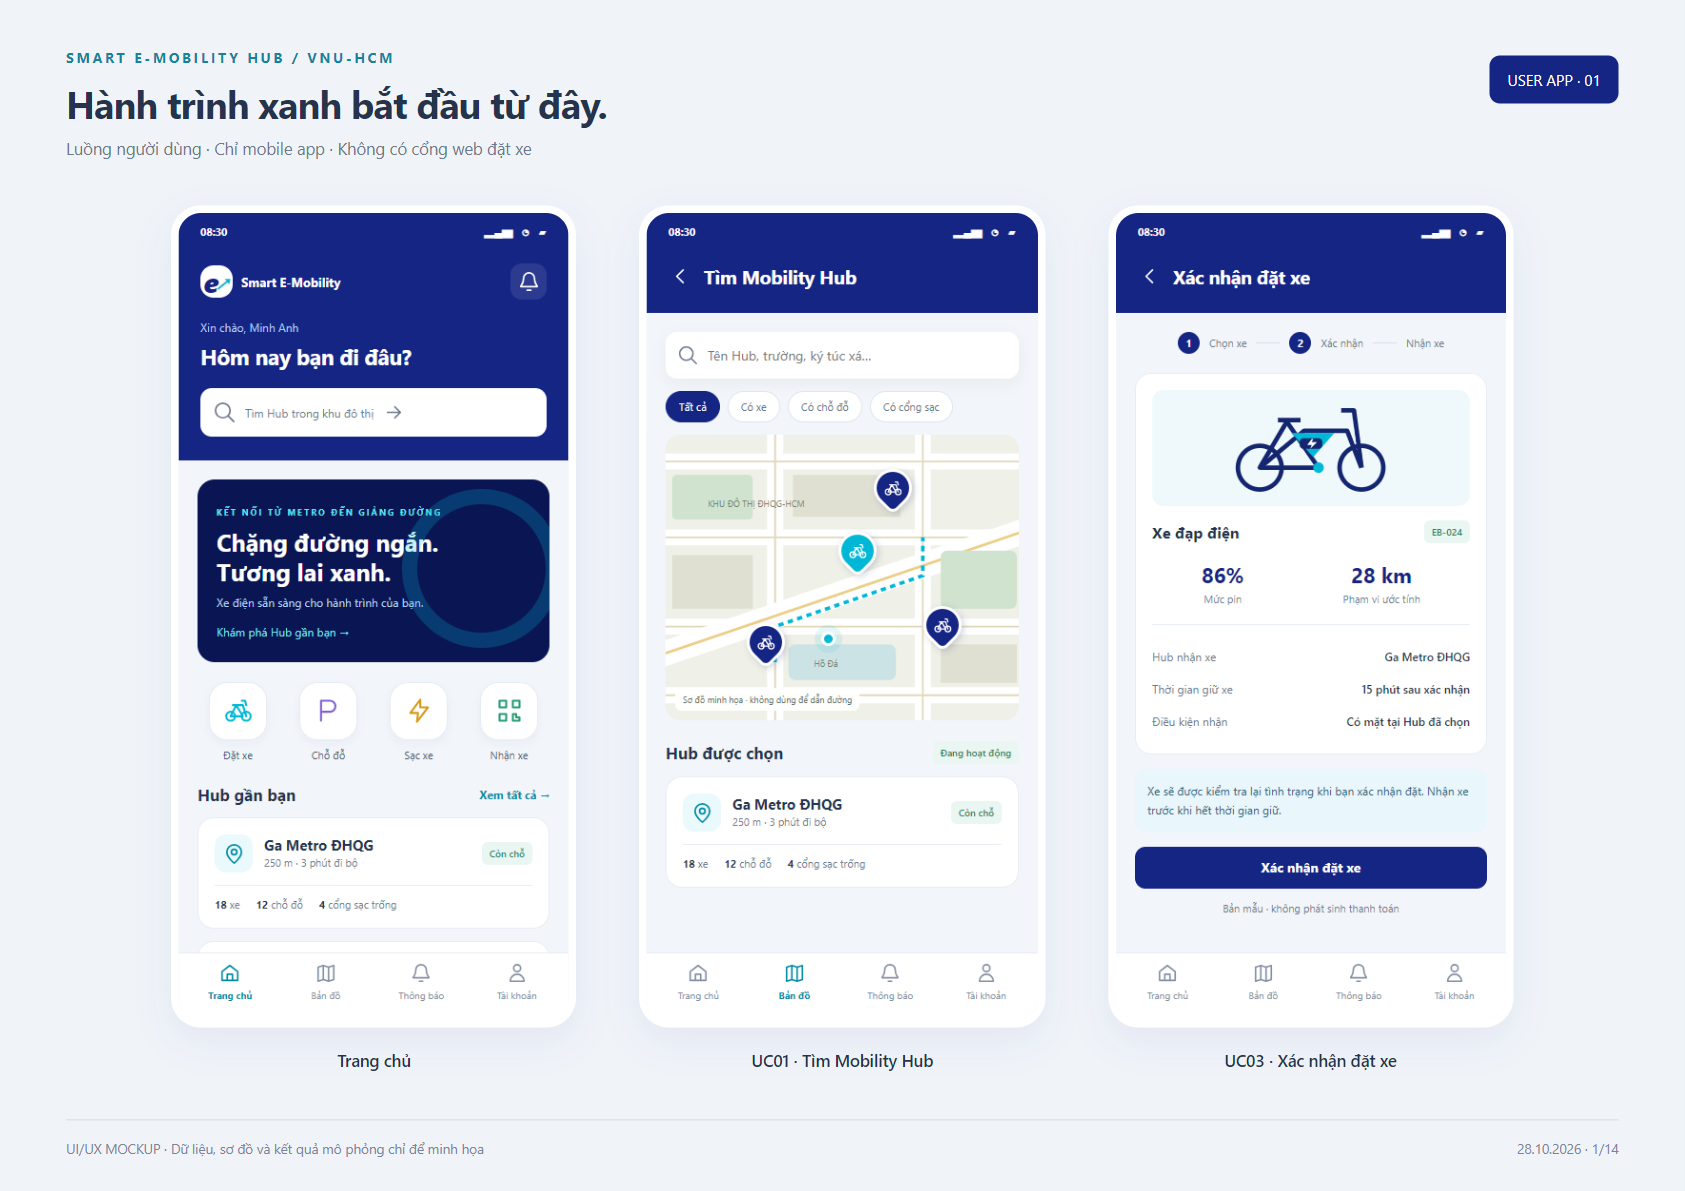
\includegraphics[width=0.95\textwidth]{../../../app/prototype/design-board.png}
    % Nguồn ảnh: app/prototype/design-board.png
    \caption{Tổng quan giao diện Mobile Người dùng (\texttt{app/prototype/design-board.png})}
    \label{fig:ui-user-board}
\end{figure}

\begin{figure}[H]
    \centering
    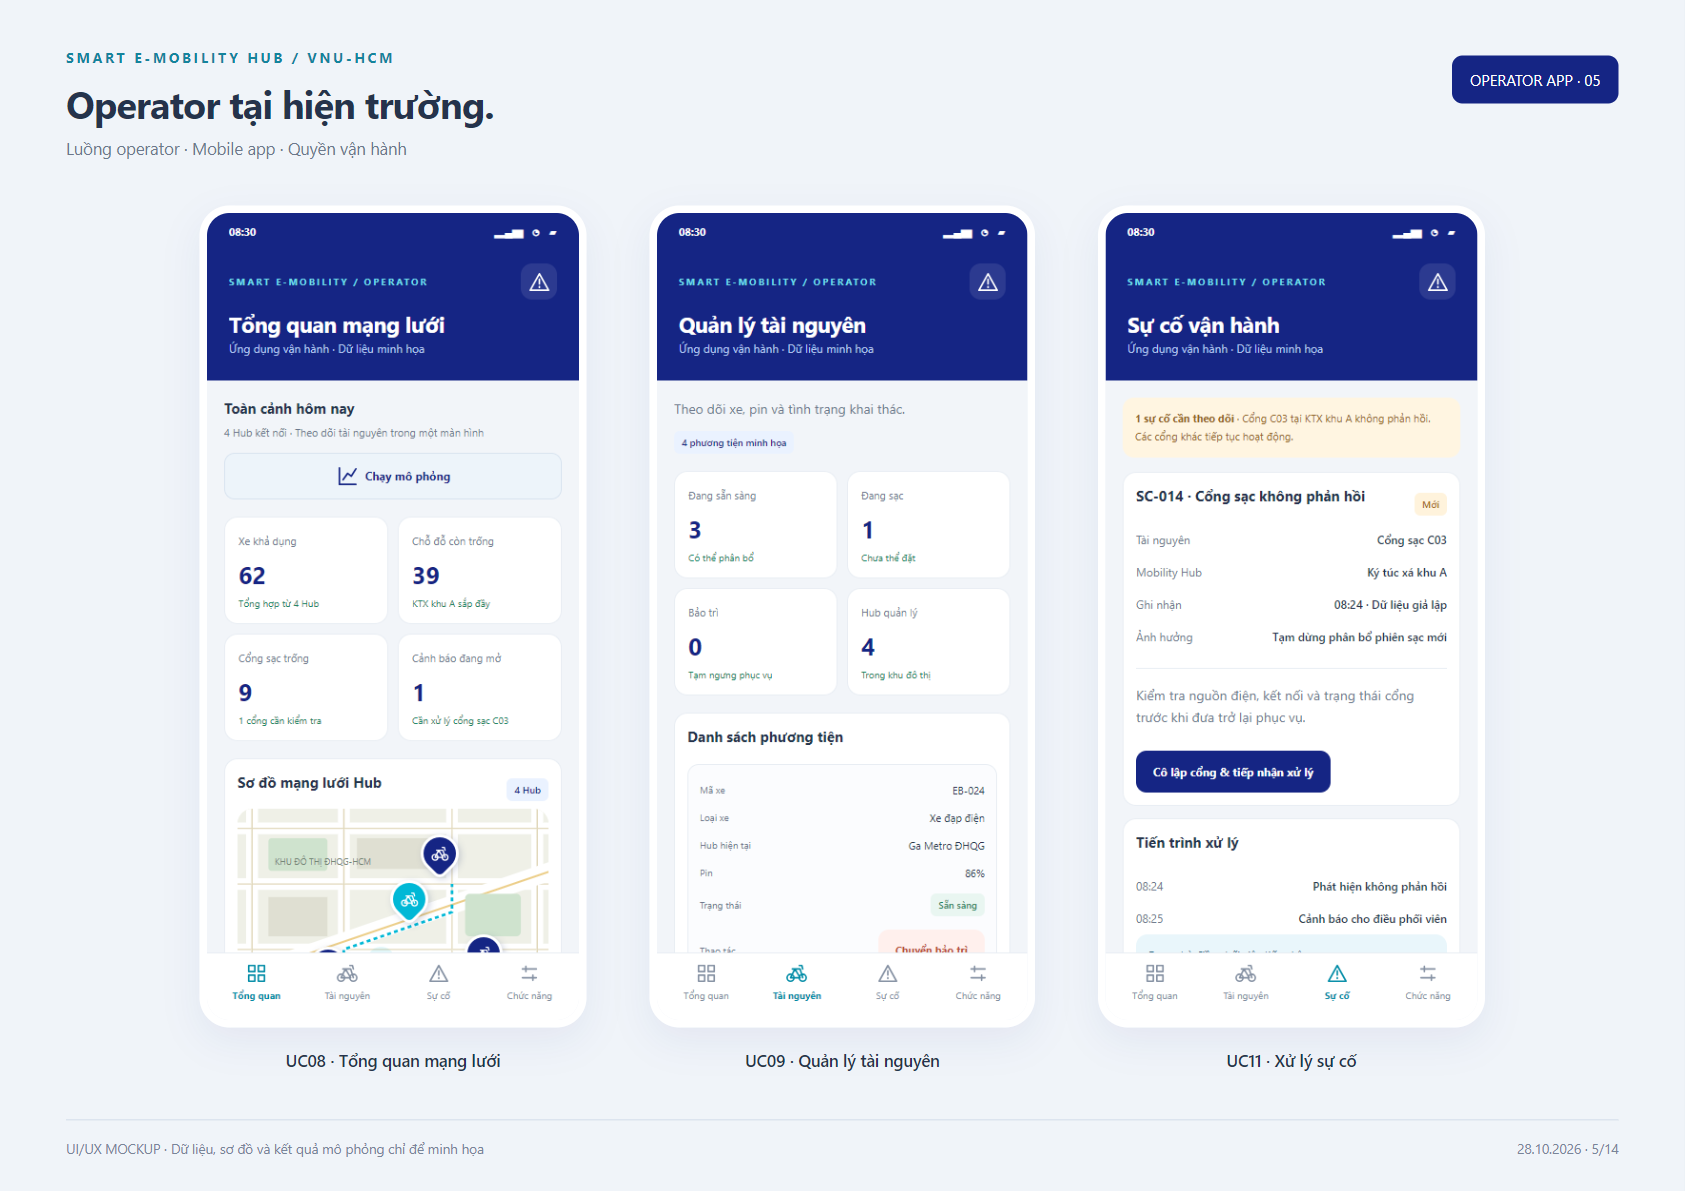
\includegraphics[width=0.95\textwidth]{../../../app/prototype/operator-app-board.png}
    % Nguồn ảnh: app/prototype/operator-app-board.png
    \caption[Tổng quan giao diện Mobile và Web Vận hành]{Tổng quan giao diện Mobile và Web Vận hành (\texttt{app/prototype/operator-app-board.png})}
    \label{fig:ui-operator-board}
\end{figure}

\subsubsection*{Ánh xạ 14 Use Cases sang 26 Màn hình và Kiểm định Playwright}
\Cref{tab:ui-26-screens} đối chiếu toàn bộ 26 tệp ảnh giao diện tại \texttt{app/prototype/screens/} với mã Use Case tương ứng. Bộ kiểm thử tự động \texttt{app/prototype/verify.cjs} chạy trên Playwright xác nhận 26/26 màn hình hiển thị không lỗi JavaScript (\textit{console error}) và không tràn bố cục ngang trên cả Mobile (\texttt{390px}) và Desktop (\texttt{1280px}), kết quả lưu tại \texttt{app/prototype/verification.json} (\texttt{passed: true}).

\begin{longtable}{>{\centering\arraybackslash}p{1.4cm} >{\raggedright\arraybackslash}p{3.9cm} >{\centering\arraybackslash}p{2.1cm} >{\raggedright\arraybackslash}p{6.8cm}}
\caption{Bảng ánh xạ 14 Use Cases sang 26 màn hình giao diện (\texttt{app/prototype/screens/})} \label{tab:ui-26-screens} \\
\toprule
\textbf{Mã UC} & \textbf{Nhóm nghiệp vụ} & \textbf{Nền tảng} & \textbf{Màn hình và tệp ảnh (\texttt{screens/})} \\
\midrule
\endfirsthead
\toprule
\textbf{Mã UC} & \textbf{Nhóm nghiệp vụ} & \textbf{Nền tảng} & \textbf{Màn hình và tệp ảnh (\texttt{screens/})} \\
\midrule
\endhead
\bottomrule
\endfoot
-- & Trang chủ, Thông báo, Tài khoản & Mobile User & \texttt{home.png}, \texttt{notifications.png}, \texttt{account.png} \\
\texttt{UC01} & Tìm kiếm Hub di chuyển & Mobile User & \texttt{map.png} (\texttt{\#map}) \\
\texttt{UC02} & Xem xe khả dụng & Mobile User & \texttt{vehicles.png} (\texttt{\#vehicles}) \\
\texttt{UC03} & Đặt giữ xe và Phiếu giữ & Mobile User & \texttt{reserve.png}, \texttt{ticket.png} \\
\texttt{UC04} & Nhận xe tại Hub & Mobile User & \texttt{pickup.png} (\texttt{\#pickup}) \\
\texttt{UC05} & Hành trình và Trả xe & Mobile User & \texttt{trip.png} (\texttt{\#trip}) \\
\texttt{UC06} & Đặt chỗ đỗ xe cá nhân & Mobile User & \texttt{parking.png} (\texttt{\#parking}) \\
\texttt{UC07} & Yêu cầu sạc điện & Mobile User & \texttt{charging.png} (\texttt{\#charging}) \\
\texttt{UC08} & Giám sát mạng lưới Hub & Web \& Mob Op & \texttt{overview.png}, \texttt{op-mobile-overview.png} \\
\texttt{UC09} & Quản lý tài nguyên & Web \& Mob Op & \texttt{resources.png}, \texttt{op-mobile-resources.png} \\
\texttt{UC10} & Điều phối cân bằng xe & Web \& Mob Op & \texttt{redistribute.png}, \texttt{op-mobile-redistribute.png} \\
\texttt{UC11} & Xử lý sự cố vận hành & Web \& Mob Op & \texttt{incidents.png}, \texttt{op-mobile-incidents.png} \\
\texttt{UC12} & Quản lý lịch sạc & Web \& Mob Op & \texttt{schedule.png}, \texttt{op-mobile-schedule.png} \\
\texttt{UC13} & Chạy mô phỏng What-if & Web \& Mob Op & \texttt{simulation.png}, \texttt{op-mobile-simulation.png} \\
\texttt{UC14} & Xem kết quả mô phỏng & Web \& Mob Op & \texttt{results.png}, \texttt{op-mobile-results.png} \\
-- & Menu điều hướng Operator & Mobile Op & \texttt{op-mobile-op-menu.png} (\texttt{\#op-menu}) \\
\end{longtable}

\subsubsection*{Luồng Chuyển màn hình (Screen Flow) và Thành phần Tương tác Cốt lõi}

Để liên kết 26 màn hình rời rạc thành chuỗi tác nghiệp khép kín, \Cref{tab:screen-flow} tóm tắt các tuyến điều hướng chính và \Cref{tab:ui-components} chú thích các thành phần điều khiển trọng tâm trên những màn hình tiêu biểu.

\begin{table}[H]
\centering
\caption{Tổng hợp luồng chuyển màn hình (Screen Flow) trên hai phân hệ}
\label{tab:screen-flow}
\begin{tabularx}{\textwidth}{>{\raggedright\arraybackslash}p{3.5cm} >{\raggedright\arraybackslash}p{4.8cm} >{\raggedright\arraybackslash}X}
\toprule
\textbf{Luồng nghiệp vụ} & \textbf{Chuỗi điều hướng màn hình} & \textbf{Điều kiện chuyển tiếp chính} \\
\midrule
Thuê -- Trả xe dùng chung (\texttt{UC01--05, 11A}) & \texttt{\#home} $\to$ \texttt{\#map} $\to$ \texttt{\#vehicles} $\to$ \texttt{\#reserve} $\to$ \texttt{\#ticket} $\to$ \texttt{\#pickup} $\to$ \texttt{\#trip} & Chọn Hub $\to$ chọn xe pin $\ge 20\%$ $\to$ khóa giữ 15 phút $\to$ quét QR/nhập mã mở khóa $\to$ trả xe vào slot trống (hoặc báo sự cố giữa chuyến). \\
\addlinespace[3pt]
Đỗ -- Sạc xe cá nhân (\texttt{UC06--07A}) & \texttt{\#home} $\to$ \texttt{\#parking} $\to$ \texttt{\#charging} & Chọn pool đỗ ngay/đặt trước $\to$ check-in tạo chiếm dụng $\to$ gửi yêu cầu sạc $\to$ dừng chủ động hoặc hoàn tất. \\
\addlinespace[3pt]
Vận hành Hiện trường (\texttt{UC08--12}) & \texttt{\#overview} $\leftrightarrow$ \texttt{\#resources} / \texttt{\#redistribute} / \texttt{\#incidents} / \texttt{\#schedule} & Điều hướng trực tiếp qua thanh bên Web Dashboard hoặc menu \texttt{\#op-menu} trên Operator Mobile. \\
\addlinespace[3pt]
Phân tích What-if (\texttt{UC13--14}) & \texttt{\#simulation} $\to$ \texttt{\#results} $\to$ \texttt{\#redistribute} & Chọn 1 trong 5 kịch bản $\to$ xem chỉ số và khuyến nghị $\to$ chuyển phương án sang biểu mẫu lập lệnh điều chuyển. \\
\bottomrule
\end{tabularx}
\end{table}

\begin{table}[H]
\centering
\caption{Chú thích các thành phần điều khiển trọng tâm trên giao diện}
\label{tab:ui-components}
\begin{tabularx}{\textwidth}{>{\raggedright\arraybackslash}p{3.4cm} >{\raggedright\arraybackslash}p{3.6cm} >{\raggedright\arraybackslash}X}
\toprule
\textbf{Màn hình / Vùng} & \textbf{Thành phần UI} & \textbf{Chức năng và Ràng buộc tương tác} \\
\midrule
\texttt{\#map}, \texttt{\#vehicles} & Thẻ Hub và Bộ lọc loại xe & Hiển thị số xe khả dụng, chỗ đỗ trống, cổng sạc; ẩn/vô hiệu hóa xe có mức pin $< 20\%$. \\
\texttt{\#ticket}, \texttt{\#pickup} & Đồng hồ đếm ngược \& Ô quét QR & Đếm ngược thời hạn giữ 15 phút; nút xác nhận mở khóa chỉ kích hoạt khi khớp mã xe và chủ phiếu. \\
\texttt{\#overview} (Operator) & Thẻ KPI và Huy hiệu cảnh báo & Làm mới định kỳ trạng thái Hub; gắn nhãn Vàng/Đỏ theo ngưỡng \texttt{BR10} và cảnh báo xung đột \texttt{LIM-01}. \\
\texttt{\#results} (Operator) & Bảng so sánh \& Nút áp dụng & Đối chiếu tỷ lệ phục vụ cơ sở -- kịch bản; nút \textit{Xem phương án điều chuyển} kiểm tra lại kho thực trước khi tạo lệnh. \\
\bottomrule
\end{tabularx}
\end{table}

\subsection{Mô hình Tương tác: Sơ đồ Tuần tự (Sequence Diagrams -- SQ01--SQ07)}

Theo bài giảng CO3001 (Ch6 tr.~21--26), nhóm xây dựng 7 sơ đồ tuần tự chuẩn UML (\texttt{SQ01--SQ07}) đặt tác nhân bên trái, phân tách lớp biên giao diện (\texttt{:MobileApp}, \texttt{:Operator\allowbreak Dashboard}), lớp điều phối nghiệp vụ (\texttt{:Reservation}, \texttt{:Pickup}, \texttt{:Return}, \texttt{:Charging}, \texttt{:Transfer}, \texttt{:Incident}, \texttt{:Simulation}) và bộ điều hợp thiết bị (\texttt{:Simulated\allowbreak Dock}, \texttt{:Simulated\allowbreak Charger}). Toàn bộ thao tác I/O với phần cứng hoặc bộ giả lập khóa chốt được đặt \textbf{bên ngoài ranh giới khóa giao dịch cơ sở dữ liệu}, tránh treo khóa ghi \texttt{BEGIN IMMEDIATE} khi thiết bị chậm phản hồi. Tổng hợp phạm vi và truy vết 7 sơ đồ tuần tự được trình bày tại \Cref{tab:sq-overview} và minh họa tại \Cref{fig:sq-01-02}--\Cref{fig:sq-05-07}.

\begin{table}[H]
\centering
\caption[Phạm vi và truy vết 7 Sơ đồ Tuần tự (\texttt{SQ01--SQ07})]{Phạm vi và truy vết 7 Sơ đồ Tuần tự (\texttt{docs/diagrams/02\_Sequence\_Diagram/drawio/})}
\label{tab:sq-overview}
\begin{tabularx}{\textwidth}{>{\centering\arraybackslash}p{1.1cm} >{\centering\arraybackslash}p{1.6cm} >{\raggedright\arraybackslash}X >{\raggedright\arraybackslash\footnotesize}p{5.5cm}}
\toprule
\textbf{Mã} & \textbf{Use Case} & \textbf{Tương tác và kết quả minh họa} & \textbf{Tệp nguồn Draw.io} \\
\midrule
\texttt{SQ01} & \texttt{UC03} & Kiểm tra điều kiện, giữ xe 15 phút và trả mã phiếu. & \texttt{SQ01-Reserve\_\allowbreak Vehicle.drawio} \\
\texttt{SQ02} & \texttt{UC04} & Đánh dấu nhận chỗ, mở khóa qua \texttt{SimulatedDock}, bắt đầu chuyến và nhả slot nguồn. & \texttt{SQ02-Pick\_Up\_\allowbreak Vehicle.drawio} \\
\texttt{SQ03} & \texttt{UC05} & Xác nhận khóa và pin tại dock, đóng chuyến và chiếm dụng slot đích. & \texttt{SQ03-Return\_\allowbreak Vehicle.drawio} \\
\texttt{SQ04} & \texttt{UC07} & Kiểm tra đầu nối và ghi yêu cầu sạc vào hàng đợi; tách biệt khỏi bước cấp điện của \texttt{UC12}. & \texttt{SQ04-Request\_\allowbreak Charging.drawio} \\
\texttt{SQ05} & \texttt{UC10} & Lập lệnh điều chuyển \texttt{Planned}, khóa xe nguồn và giữ sức chứa đích. & \texttt{SQ05-Redistribute\_\allowbreak Vehicles.drawio} \\
\texttt{SQ06} & \texttt{UC11} & Đánh giá ảnh hưởng, cô lập tài nguyên lỗi và lập lịch bảo trì lần đầu. & \texttt{SQ06-Handle\_Operational\_\allowbreak Incident.drawio} \\
\texttt{SQ07} & \texttt{UC13, UC14} & Thực thi mô phỏng trên bản chụp cô lập và hiển thị chỉ số/khuyến nghị. & \texttt{SQ07-Run\_What\_if\_\allowbreak Simulation.drawio} \\
\bottomrule
\end{tabularx}
\end{table}

\begin{figure}[H]
    \centering
        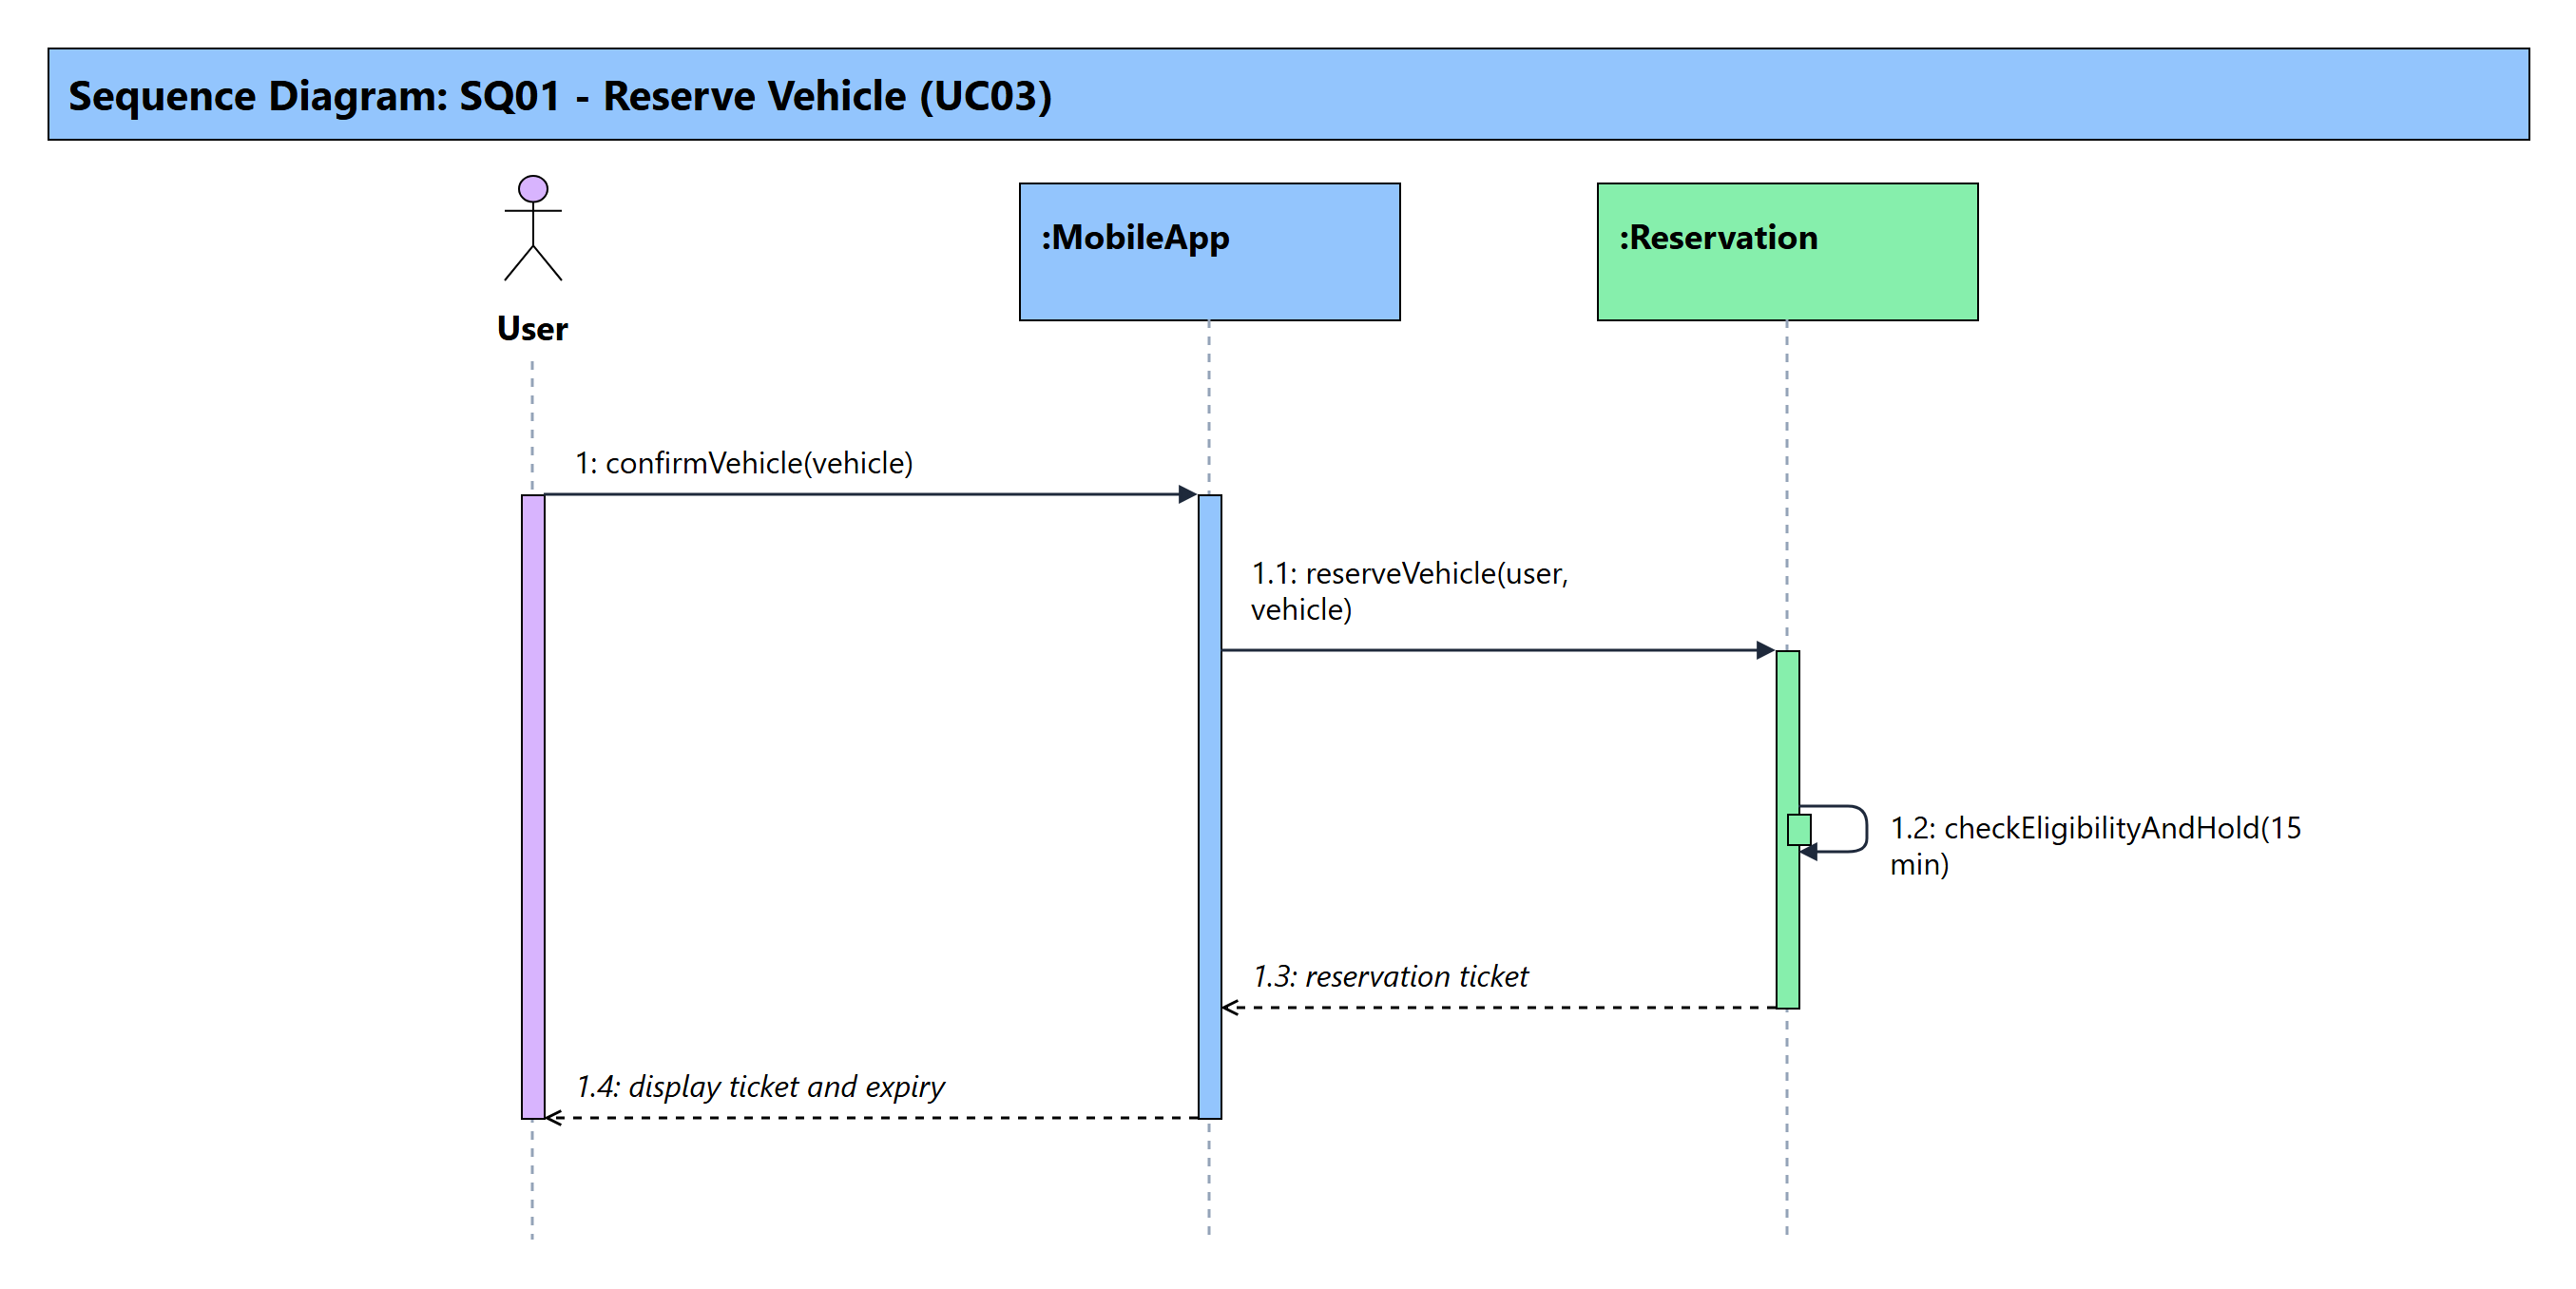
\includegraphics[width=0.92\textwidth,height=0.38\textheight,keepaspectratio]{graphics/diagrams/SQ01-Reserve_Vehicle.png}
    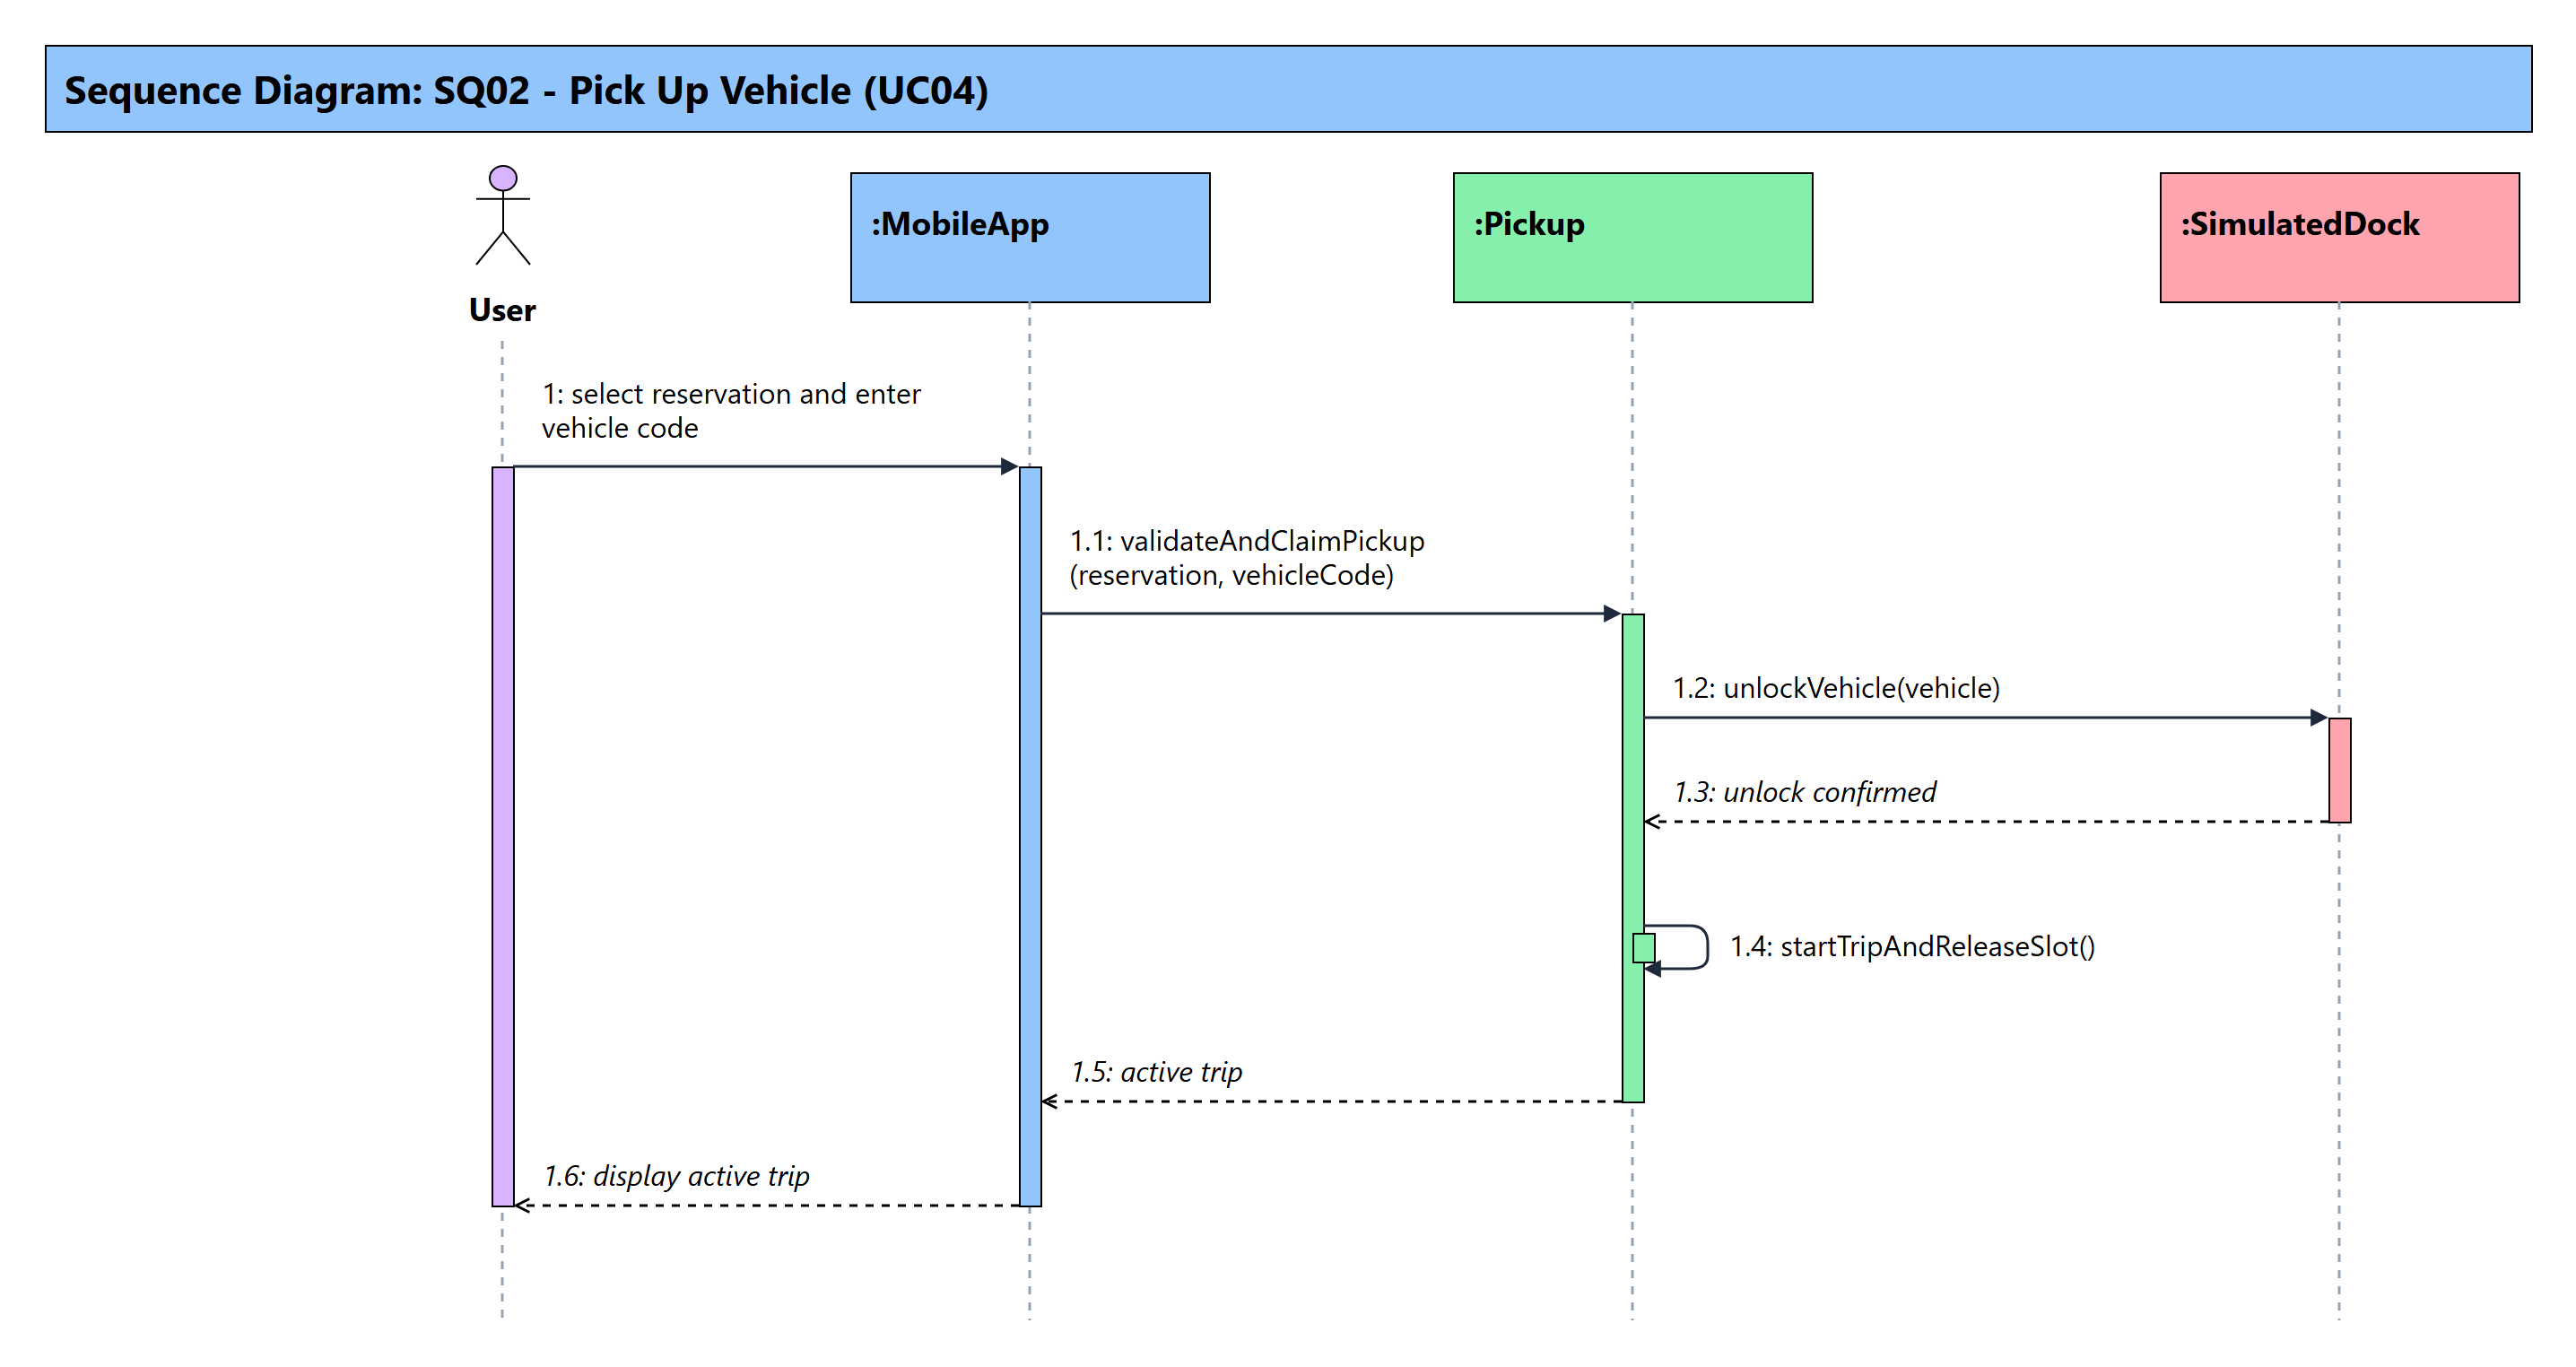
\includegraphics[width=0.92\textwidth,height=0.38\textheight,keepaspectratio]{graphics/diagrams/SQ02-Pick_Up_Vehicle.png}
    \caption{Sơ đồ tuần tự đặt giữ xe (\texttt{SQ01}) và nhận xe tại Hub (\texttt{SQ02})}
    \label{fig:sq-01-02}
\end{figure}

\begin{figure}[H]
    \centering
        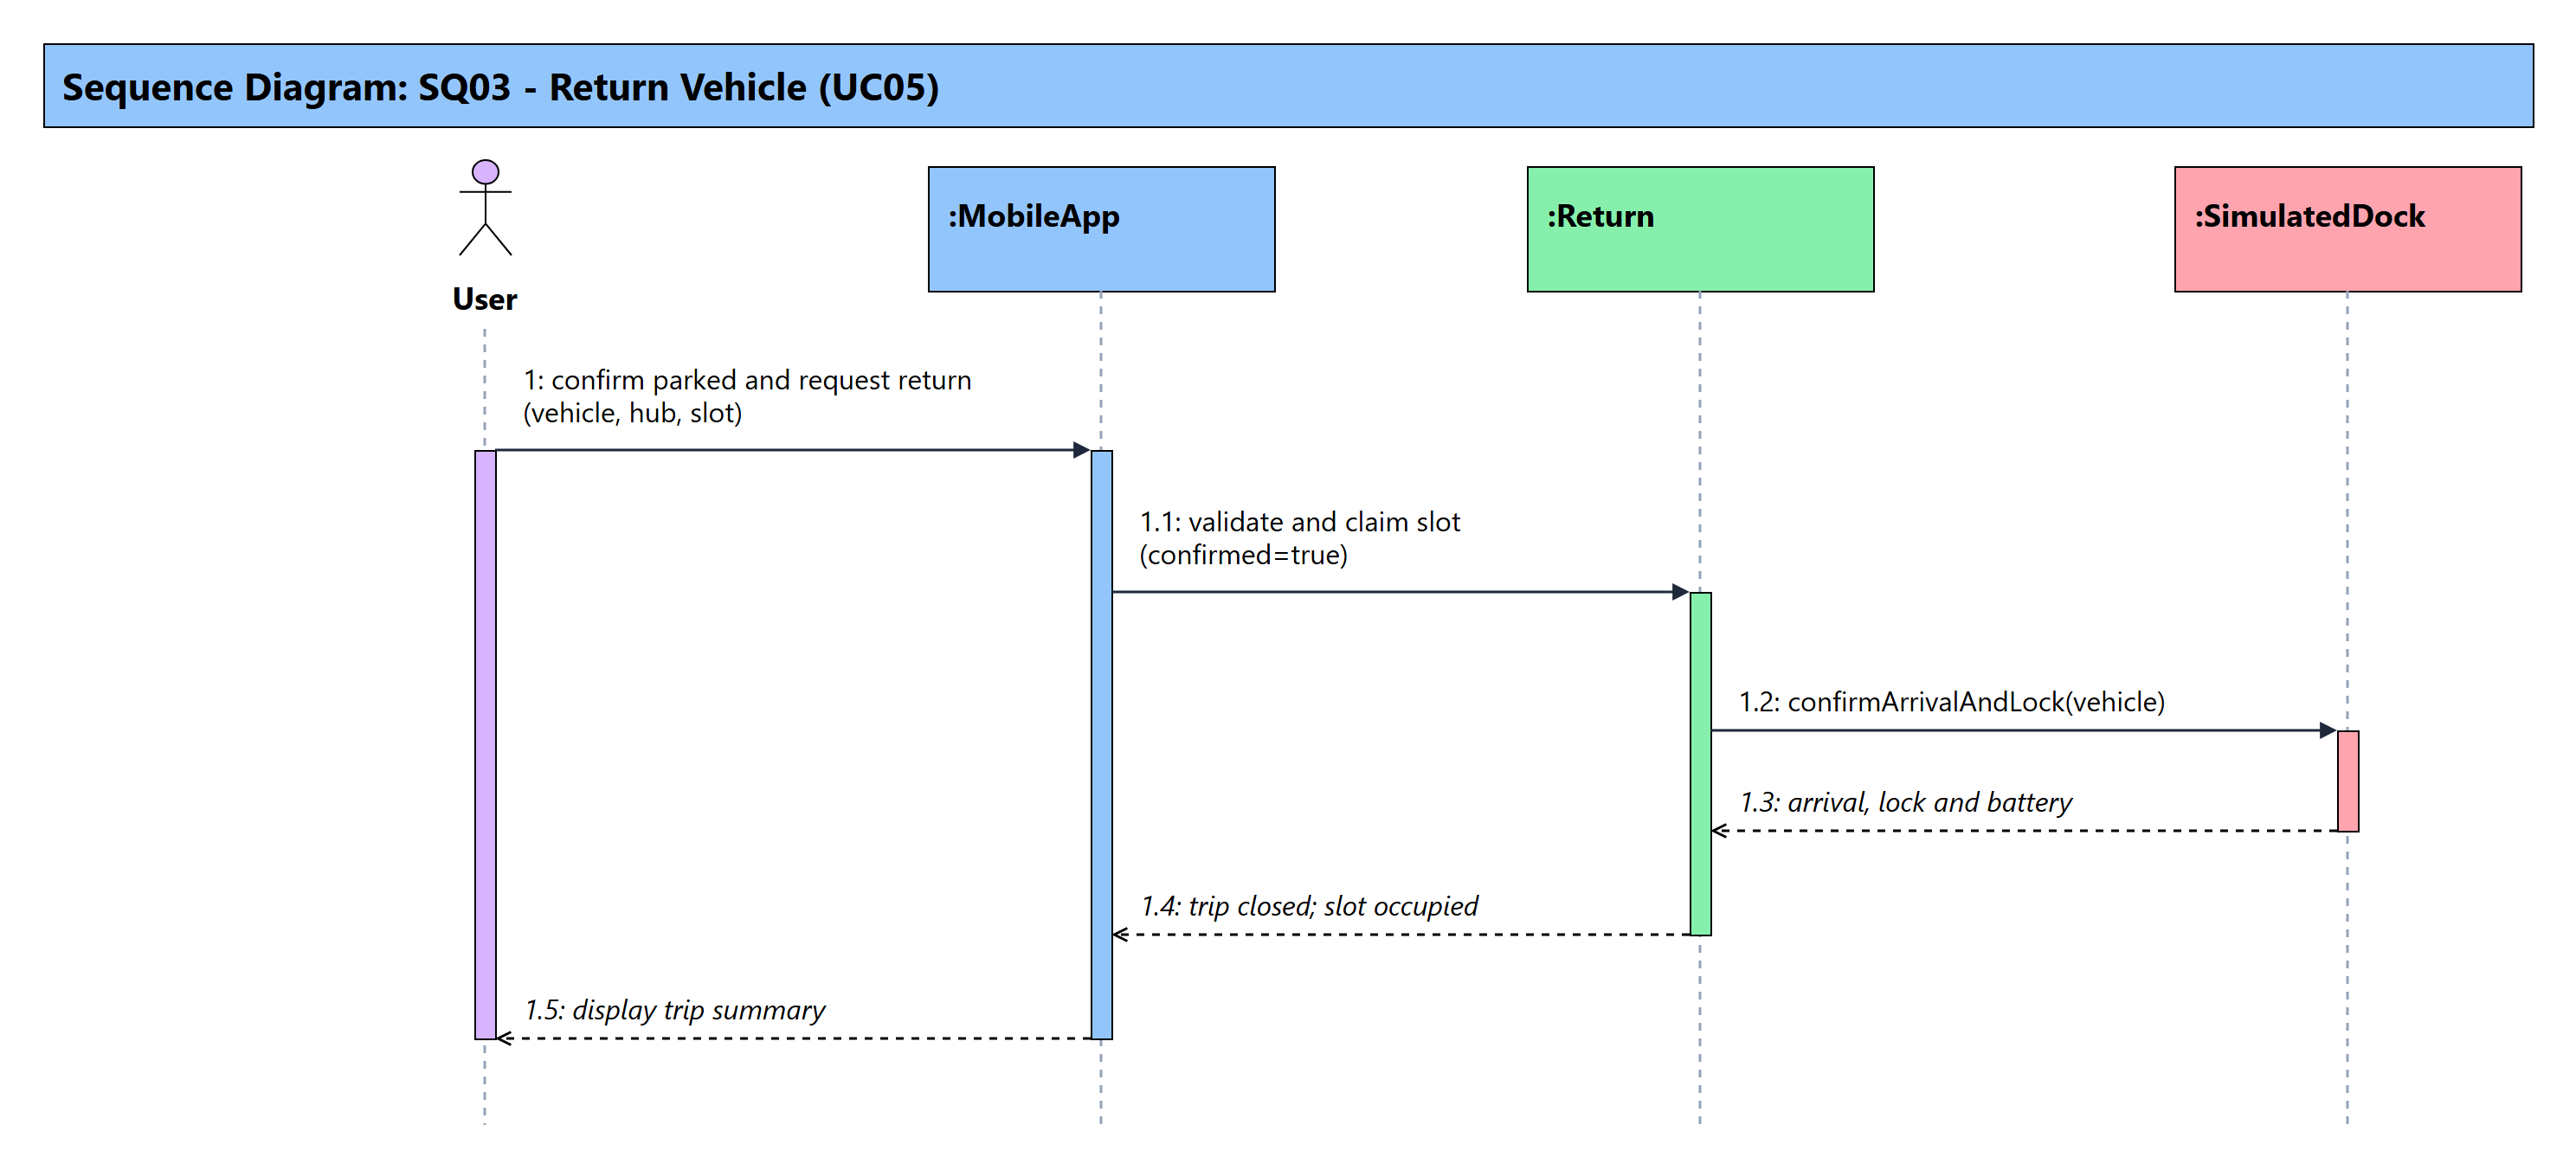
\includegraphics[width=0.92\textwidth,height=0.38\textheight,keepaspectratio]{graphics/diagrams/SQ03-Return_Vehicle.png}
    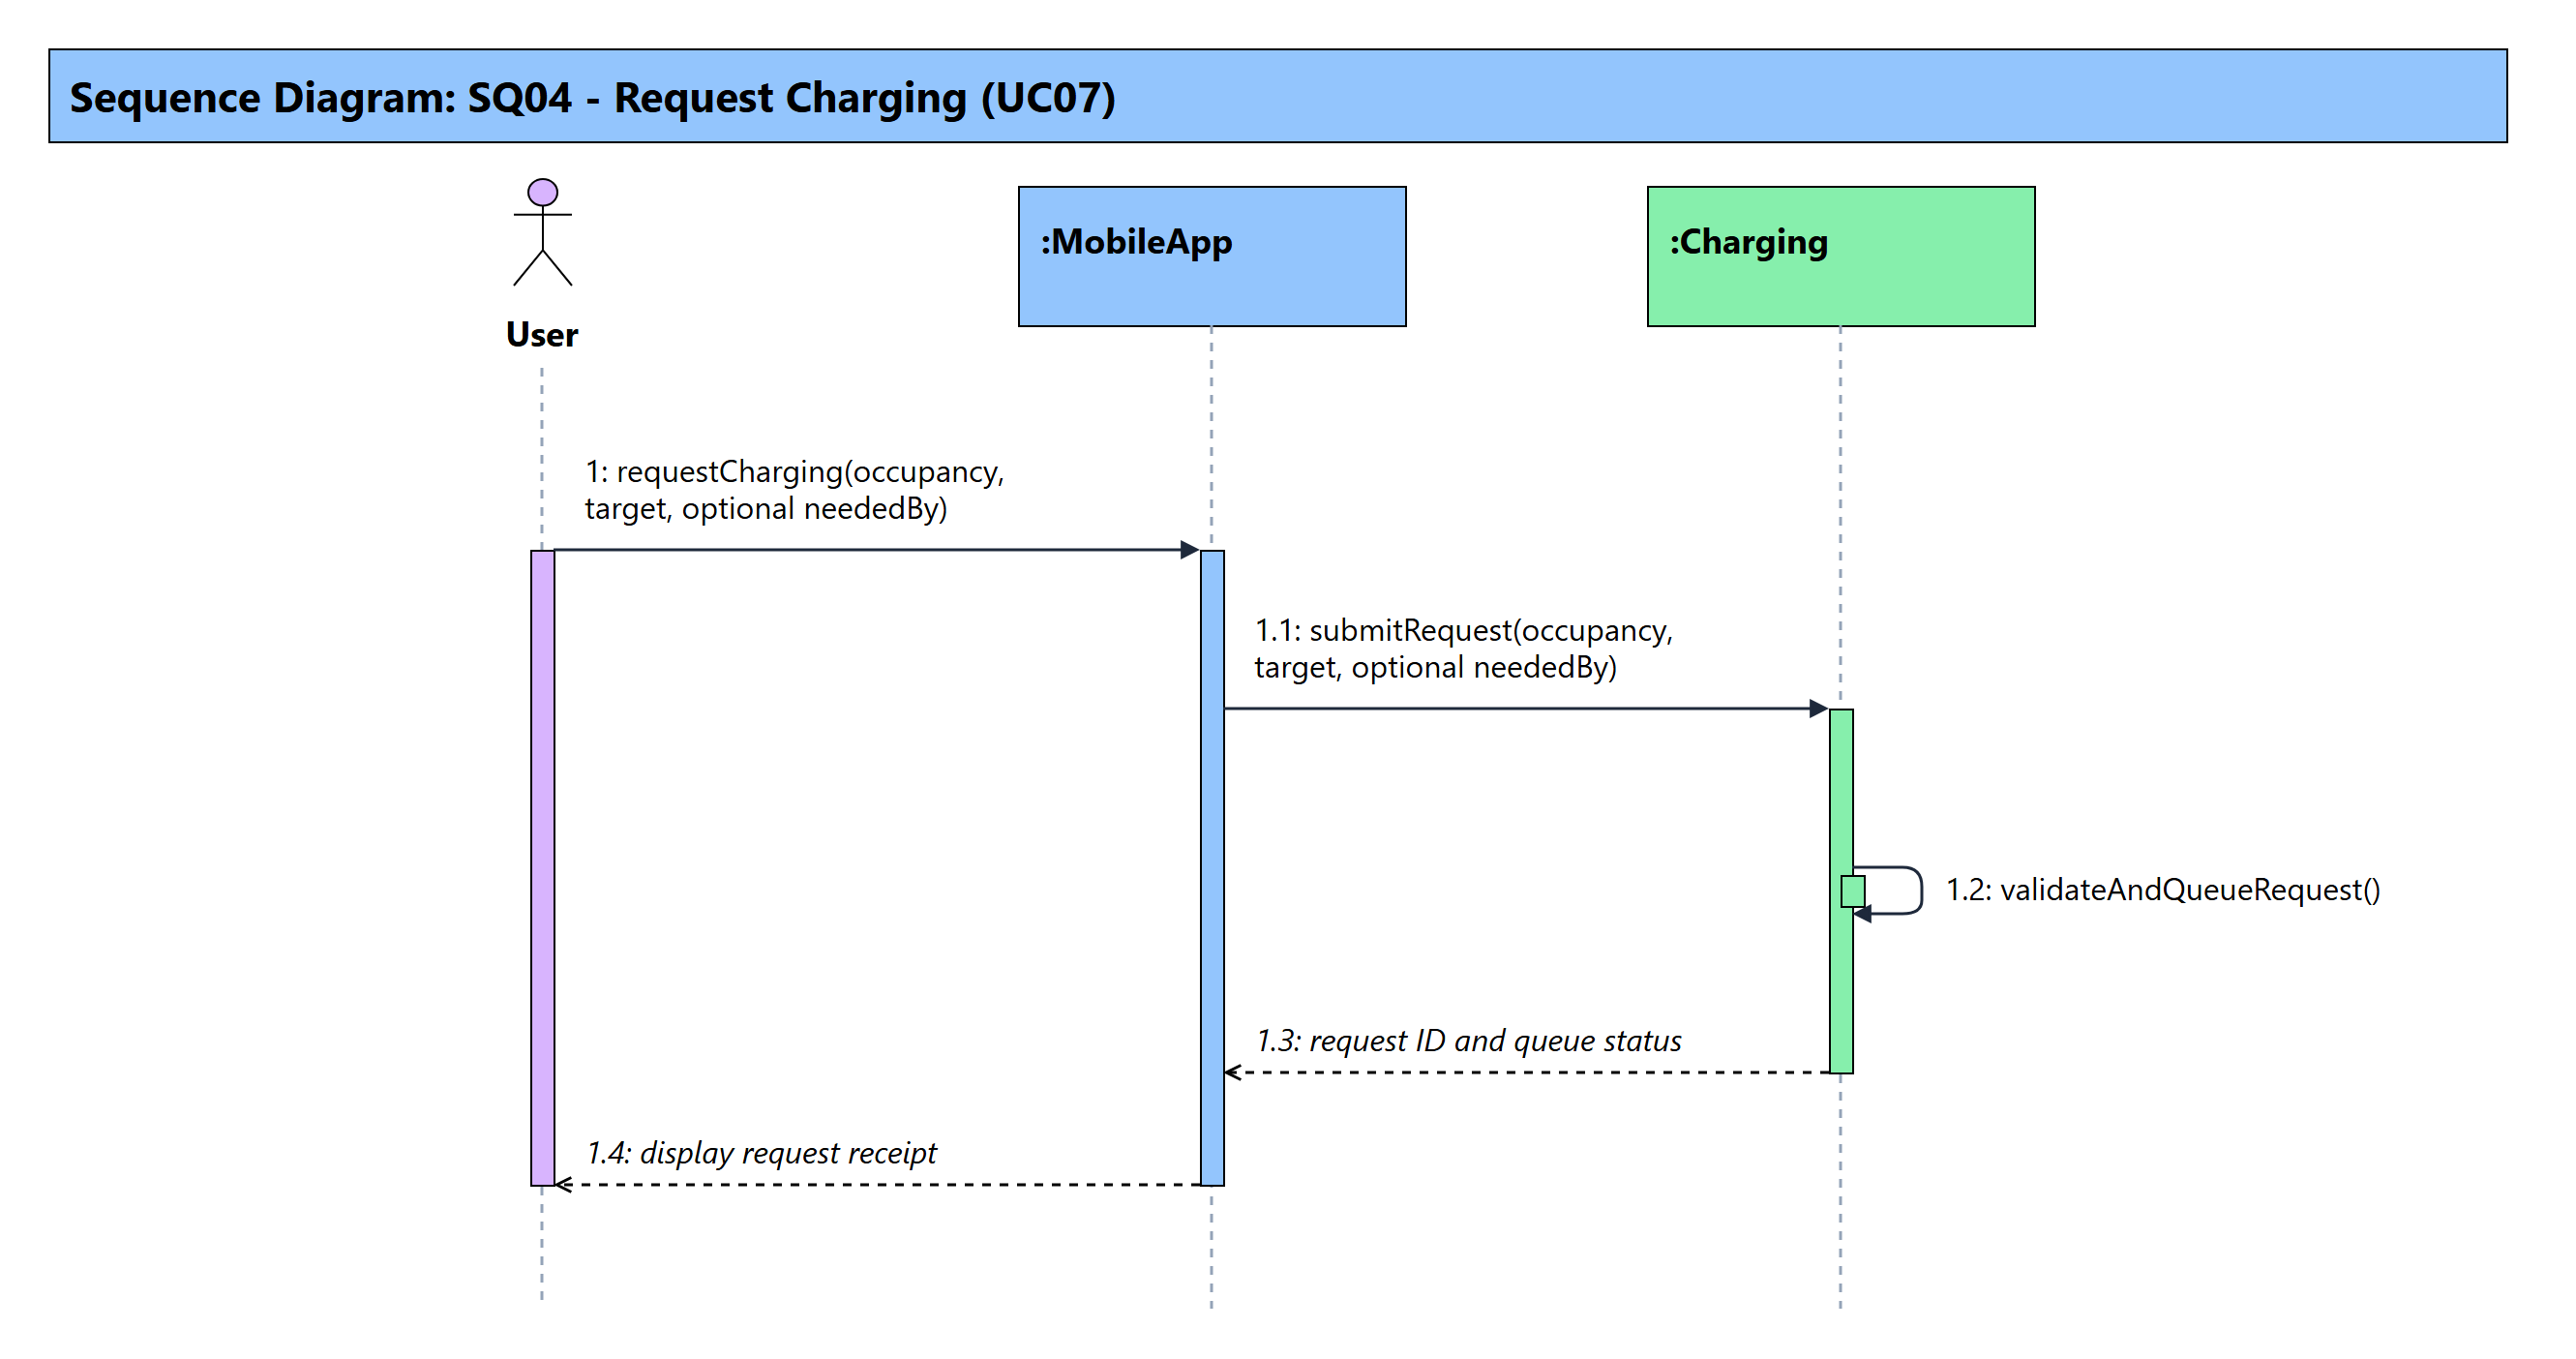
\includegraphics[width=0.92\textwidth,height=0.38\textheight,keepaspectratio]{graphics/diagrams/SQ04-Request_Charging.png}
    \caption{Sơ đồ tuần tự trả xe (\texttt{SQ03}) và tiếp nhận yêu cầu sạc (\texttt{SQ04})}
    \label{fig:sq-03-04}
\end{figure}

\begin{figure}[H]
    \centering
    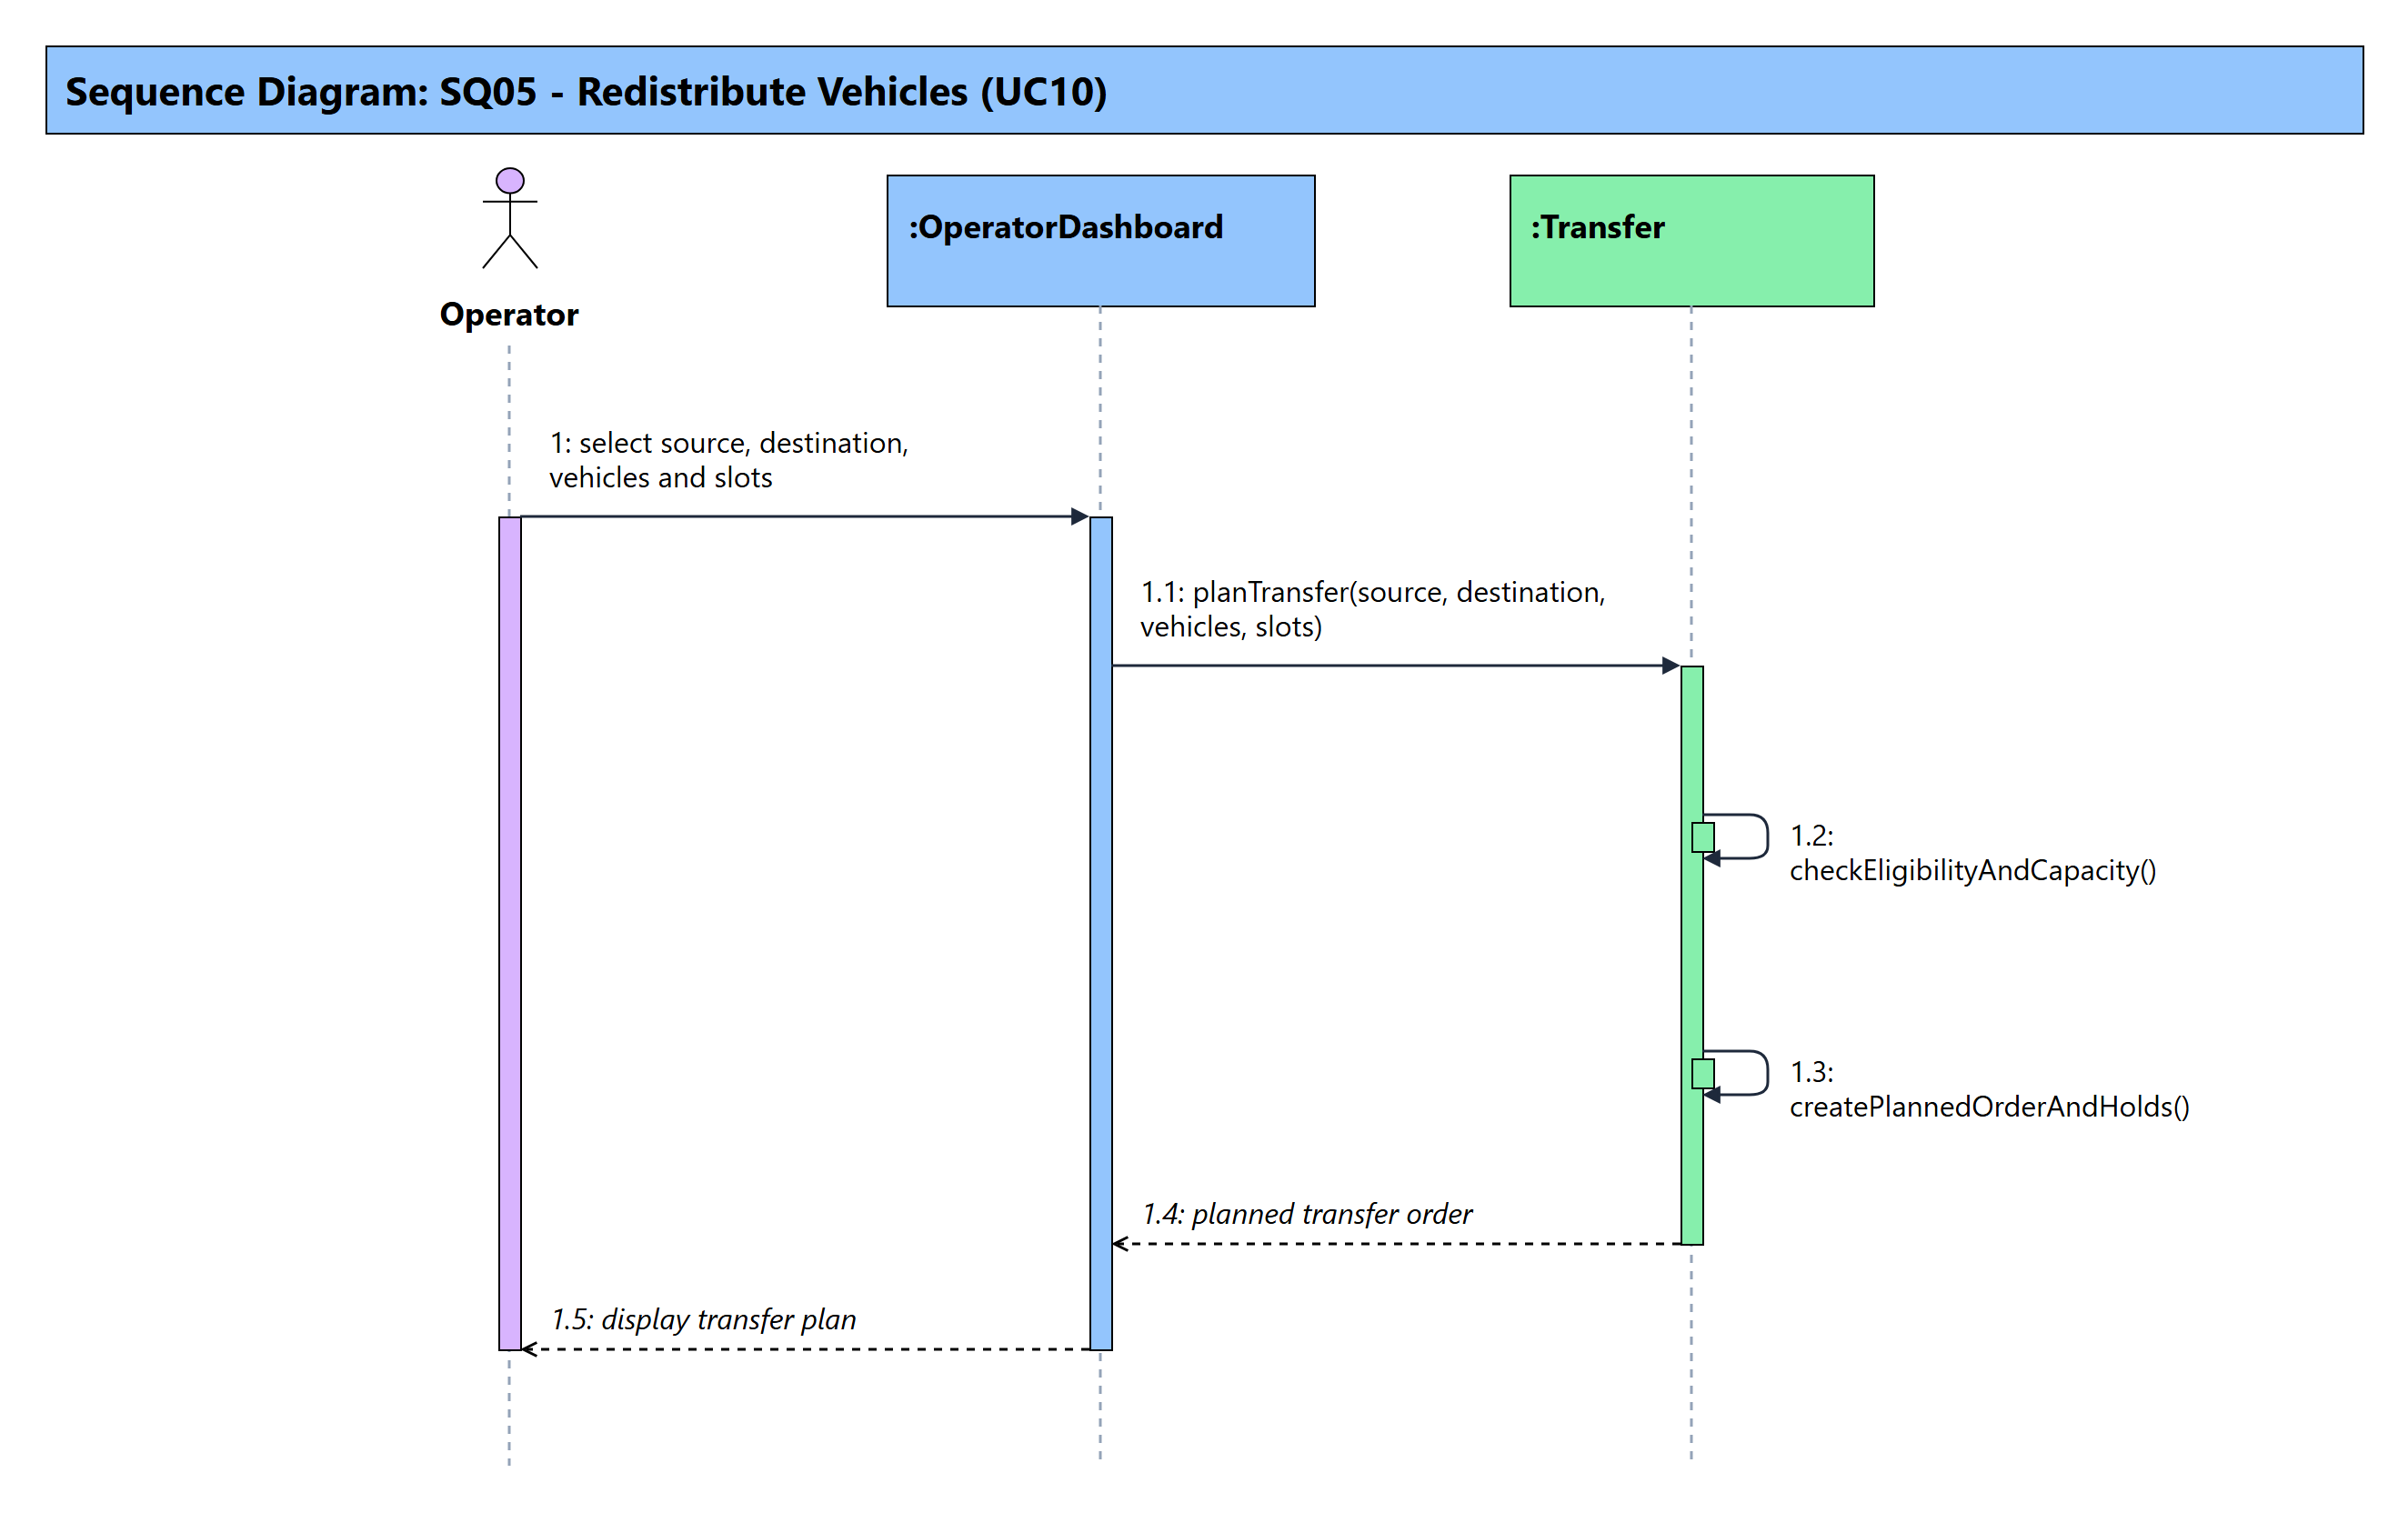
\includegraphics[width=0.92\textwidth,height=0.25\textheight,keepaspectratio]{graphics/diagrams/SQ05-Redistribute_Vehicles.png}\par\medskip
    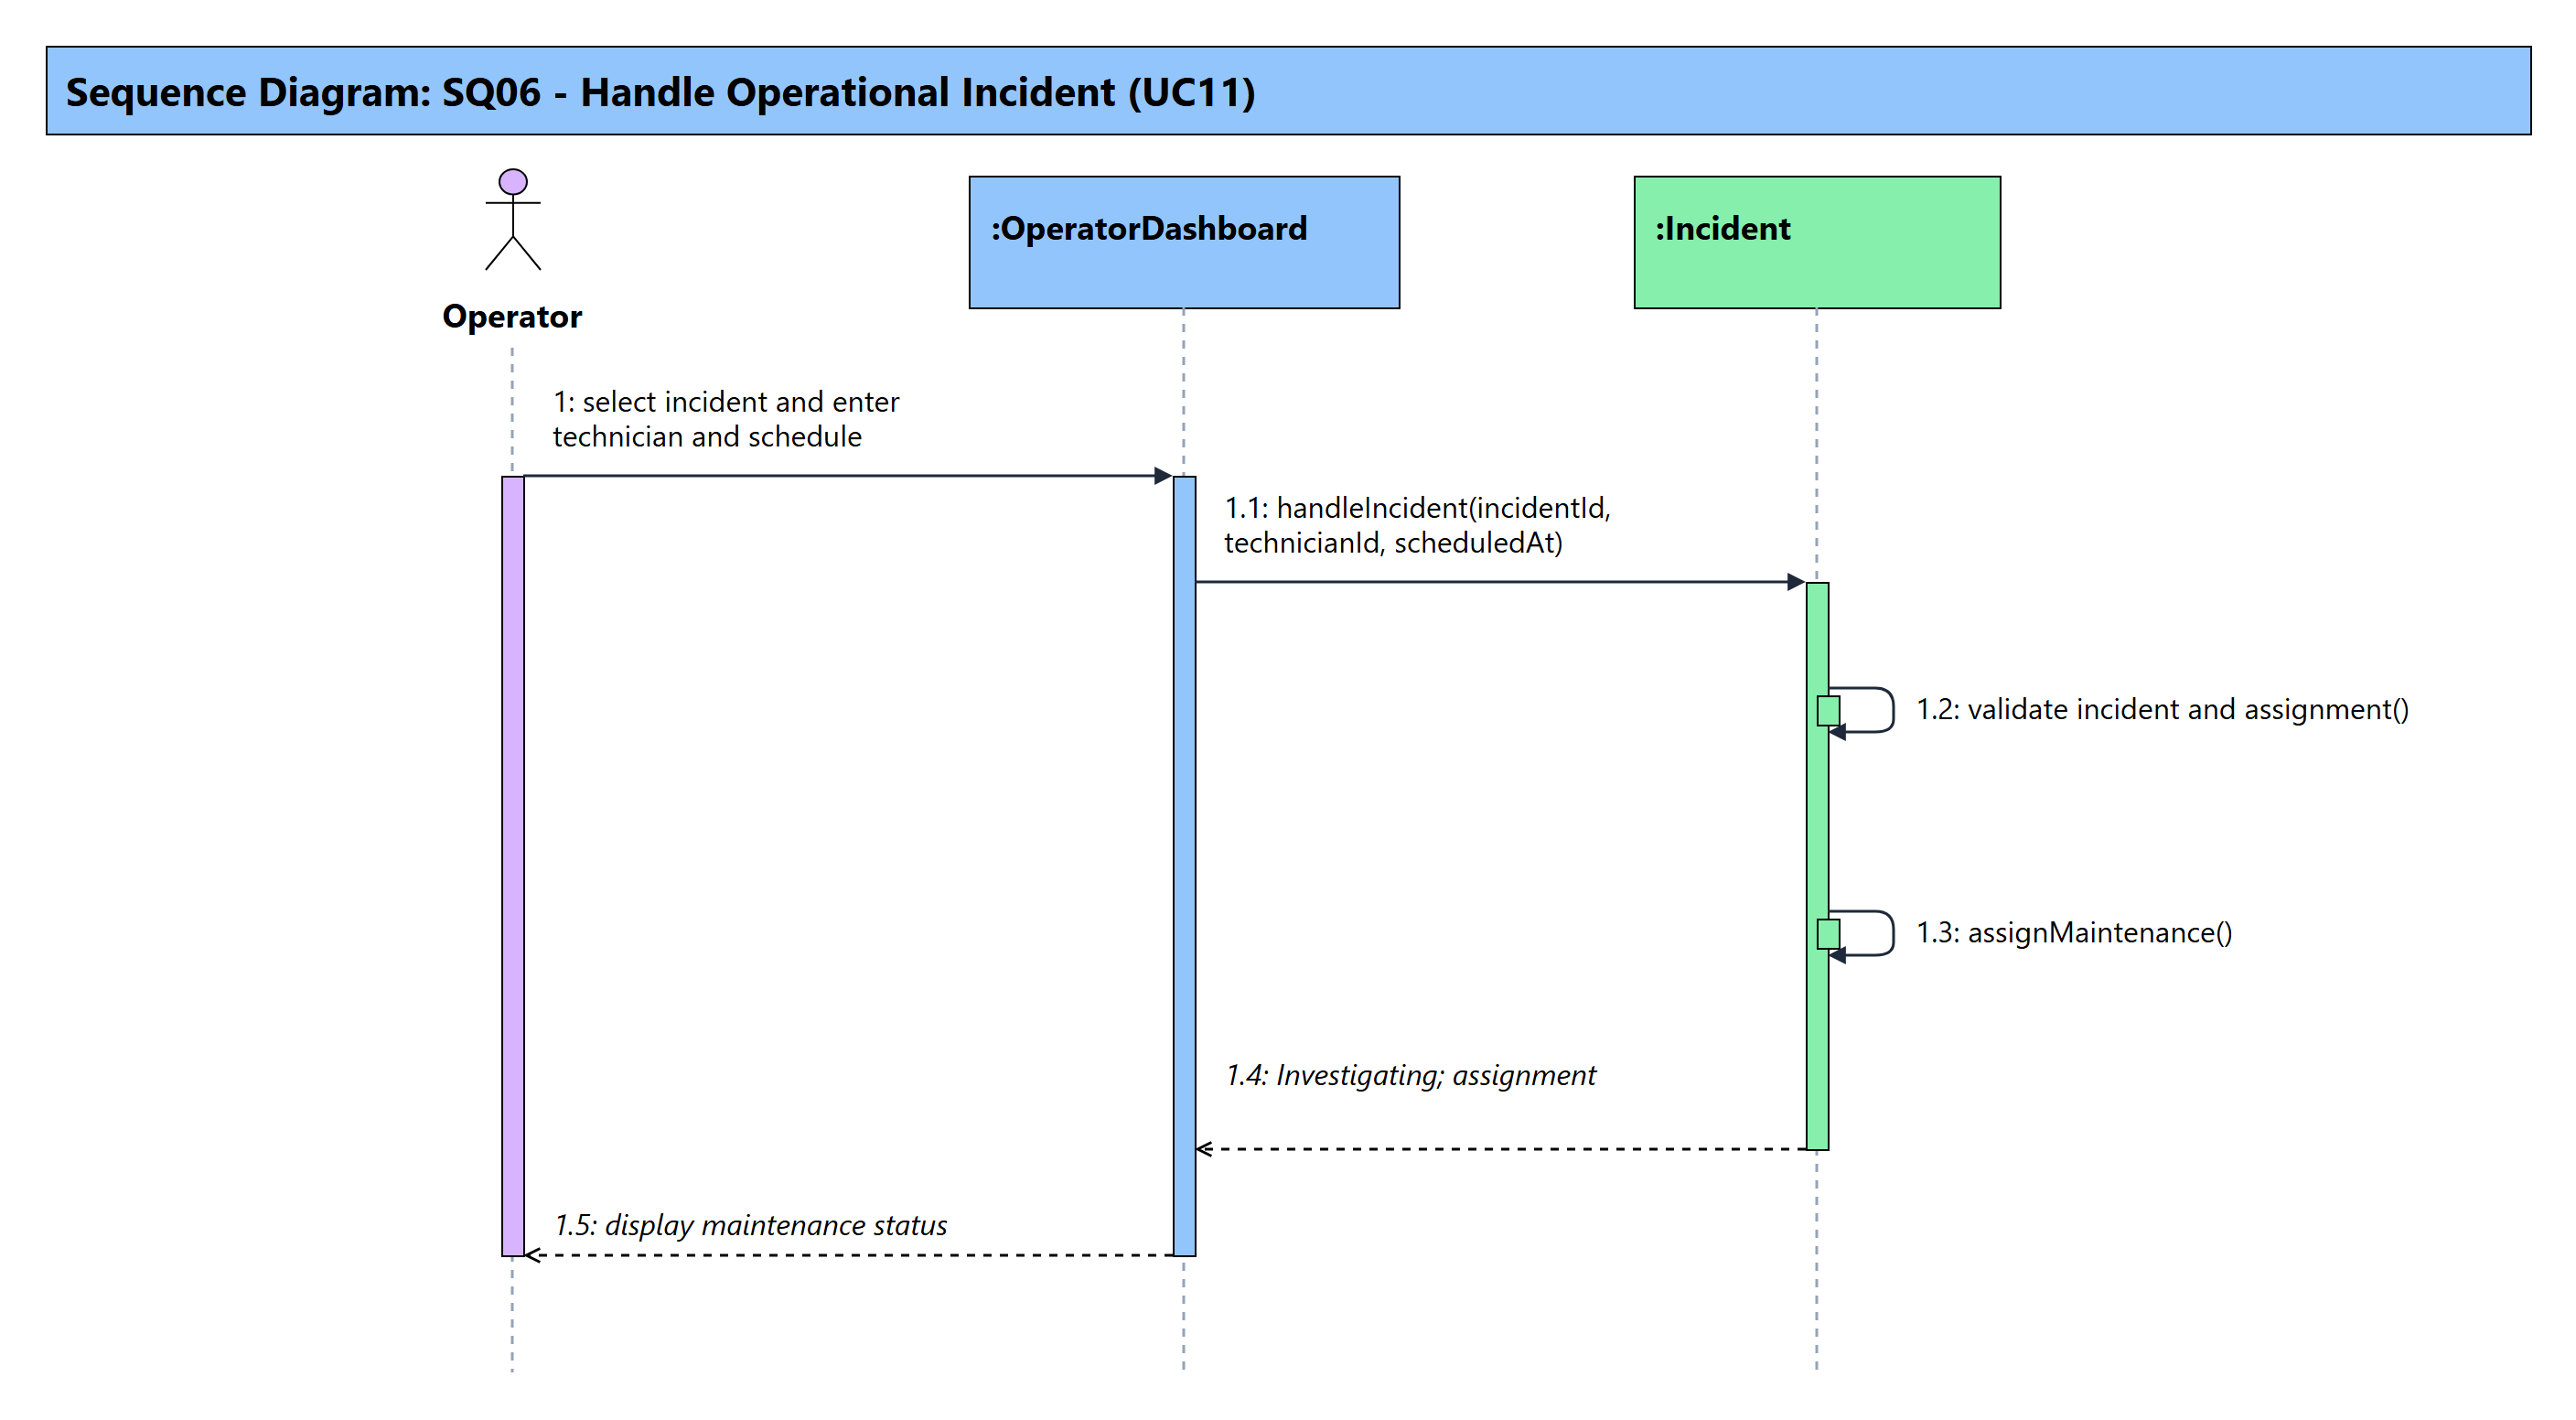
\includegraphics[width=0.92\textwidth,height=0.25\textheight,keepaspectratio]{graphics/diagrams/SQ06-Handle_Operational_Incident.png}\par\medskip
    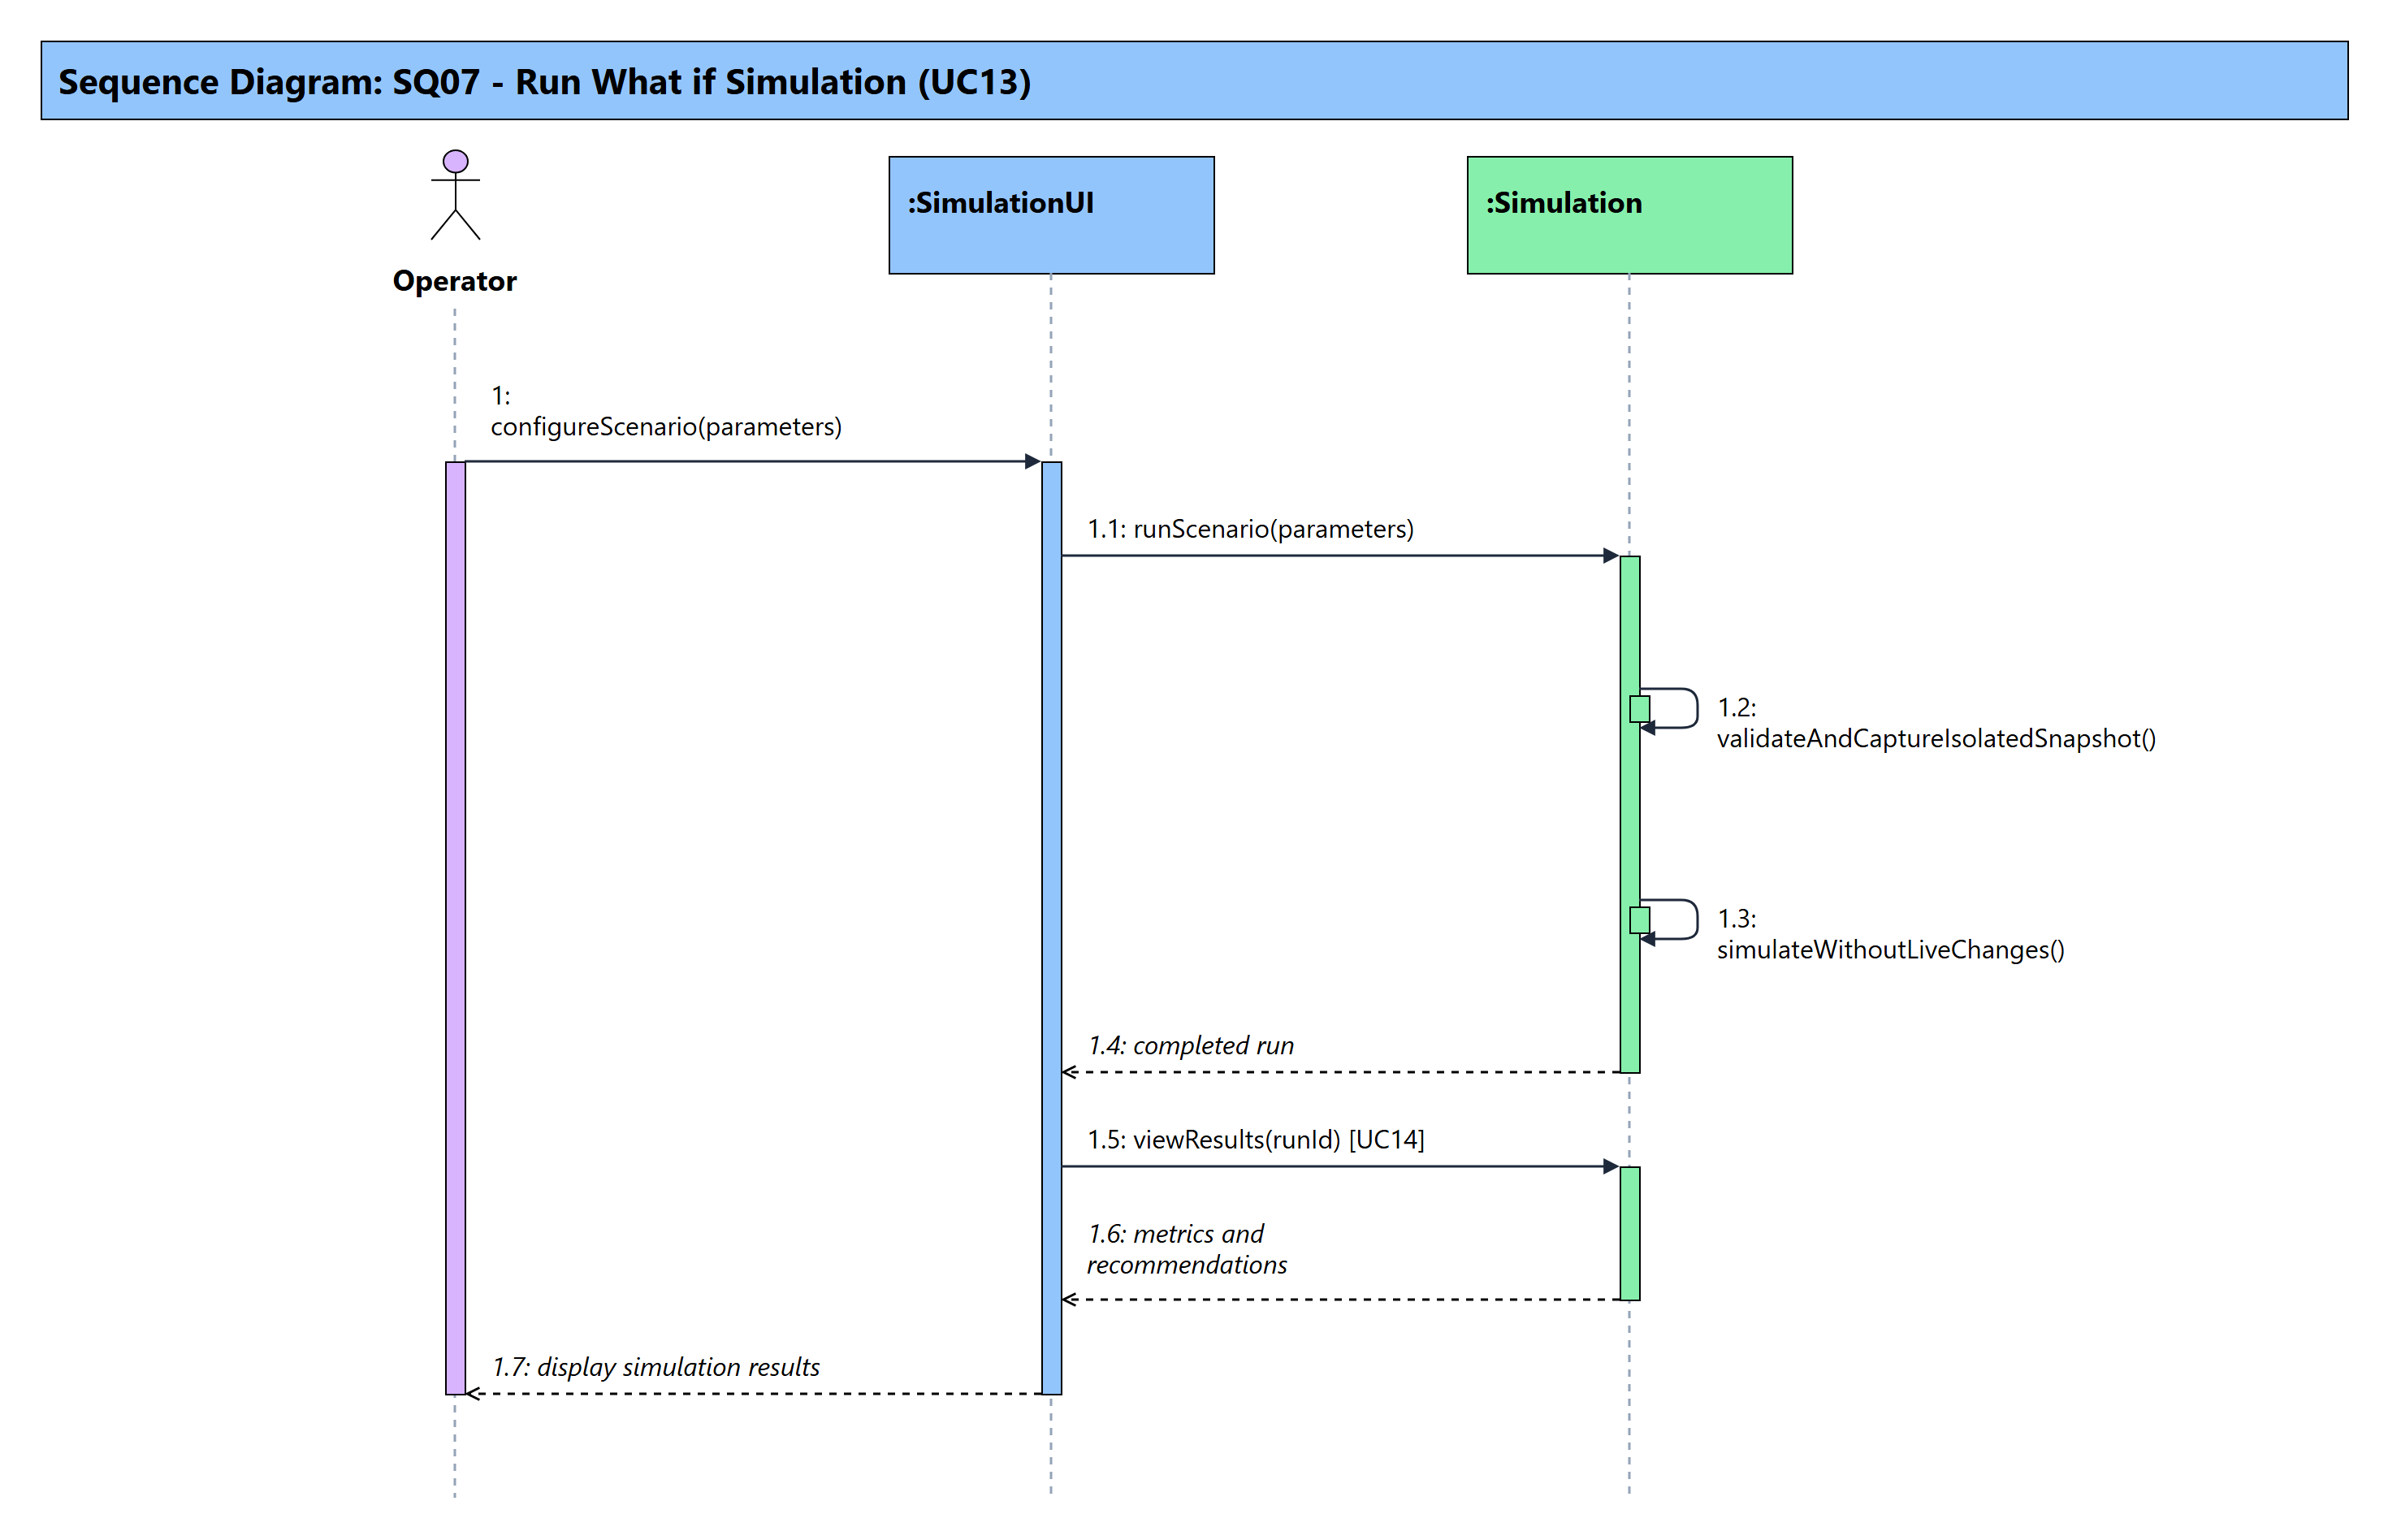
\includegraphics[width=0.92\textwidth,height=0.25\textheight,keepaspectratio]{graphics/diagrams/SQ07-Run_What_if_Simulation.png}
    \caption{Sơ đồ tuần tự điều chuyển xe (\texttt{SQ05}), xử lý sự cố (\texttt{SQ06}) và mô phỏng What-if (\texttt{SQ07})}
    \label{fig:sq-05-07}
\end{figure}

\subsection{Mô hình Hành vi: Sơ đồ Hoạt động (Activity Diagrams -- AD01--AD07)}

Bộ 7 sơ đồ hoạt động được tổ chức theo các đường bơi (\textit{Swimlanes}) phân định trách nhiệm giữa \texttt{User / App} (hoặc \texttt{Operator / App}), \texttt{Backend} và \texttt{IoT / Simulated Station}. Mọi nút rẽ nhánh đều gắn điều kiện bảo vệ (\textit{guard condition}) như \texttt{[Available, battery >=20\%, no hold]}, bảo đảm mọi nhánh xung đột hoặc ngoại lệ đều dẫn về nút kết thúc hợp lệ (\Cref{tab:ad-overview} và \Cref{fig:ad-01}--\Cref{fig:ad-07}). Đặc biệt, \texttt{AD04} tách biệt điểm bắt đầu check-in/checkout chỗ đỗ với thao tác gửi yêu cầu và dừng sạc an toàn.

\begin{table}[H]
\centering
\caption[Tổng hợp 7 Sơ đồ Hoạt động (\texttt{AD01--AD07})]{Tổng hợp 7 Sơ đồ Hoạt động và liên kết truy vết (\texttt{docs/diagrams/03\_Activity\_Diagram/drawio/})}
\label{tab:ad-overview}
\begin{tabularx}{\textwidth}{>{\centering\arraybackslash}p{1.1cm} >{\raggedright\arraybackslash}p{2.2cm} >{\raggedright\arraybackslash}X >{\raggedright\arraybackslash\footnotesize}p{5.5cm}}
\toprule
\textbf{Mã} & \textbf{Use Cases} & \textbf{Trọng tâm luồng điều khiển và ngoại lệ} & \textbf{Tệp nguồn Draw.io} \\
\midrule
\texttt{AD01} & \texttt{UC03} & Kiểm tra khả dụng, giữ xe nguyên tử 15 phút; rẽ nhánh xung đột đặt chỗ. & \texttt{AD01-Reserve\_\allowbreak Vehicle.drawio} \\
\texttt{AD02} & \texttt{UC04} & Báo hỏng trước khi lấy xe, tuần tự hóa \textit{pickupClaimed} và xử lý lỗi mở khóa. & \texttt{AD02-Pick\_Up\_\allowbreak Vehicle.drawio} \\
\texttt{AD03} & \texttt{UC05} & Kiểm tra chỗ trống Hub đích, xác minh khóa chốt và phân loại pin khi trả. & \texttt{AD03-Return\_\allowbreak Vehicle.drawio} \\
\texttt{AD04} & \texttt{UC06, UC07, UC12} & Tách biệt đặt chỗ, check-in/out xe cá nhân, quá giờ \texttt{LIM-01} và dừng sạc \texttt{UC07A}. & \texttt{AD04-Reserve\_Parking\_\allowbreak and\_Charging.drawio} \\
\texttt{AD05} & \texttt{UC10, UC10A/B} & Lập lệnh giữ xe và slot đích; cạnh tranh \textit{Depart/Cancel}; xác nhận đến đủ lô. & \texttt{AD05-Redistribute\_\allowbreak Vehicles.drawio} \\
\texttt{AD06} & \texttt{UC11, UC11A} & Cô lập trước khi bảo trì; giữ chuyến đi mở khi nhận báo cáo giữa chuyến. & \texttt{AD06-Handle\_Operational\_\allowbreak Incident.drawio} \\
\texttt{AD07} & \texttt{UC13, UC14} & Thực thi mô phỏng bản chụp cô lập; chỉ áp dụng khuyến nghị sau kiểm tra thực. & \texttt{AD07-Run\_What\_if\_\allowbreak Simulation.drawio} \\
\bottomrule
\end{tabularx}
\end{table}

\clearpage
\begin{figure}[H]
    \centering
    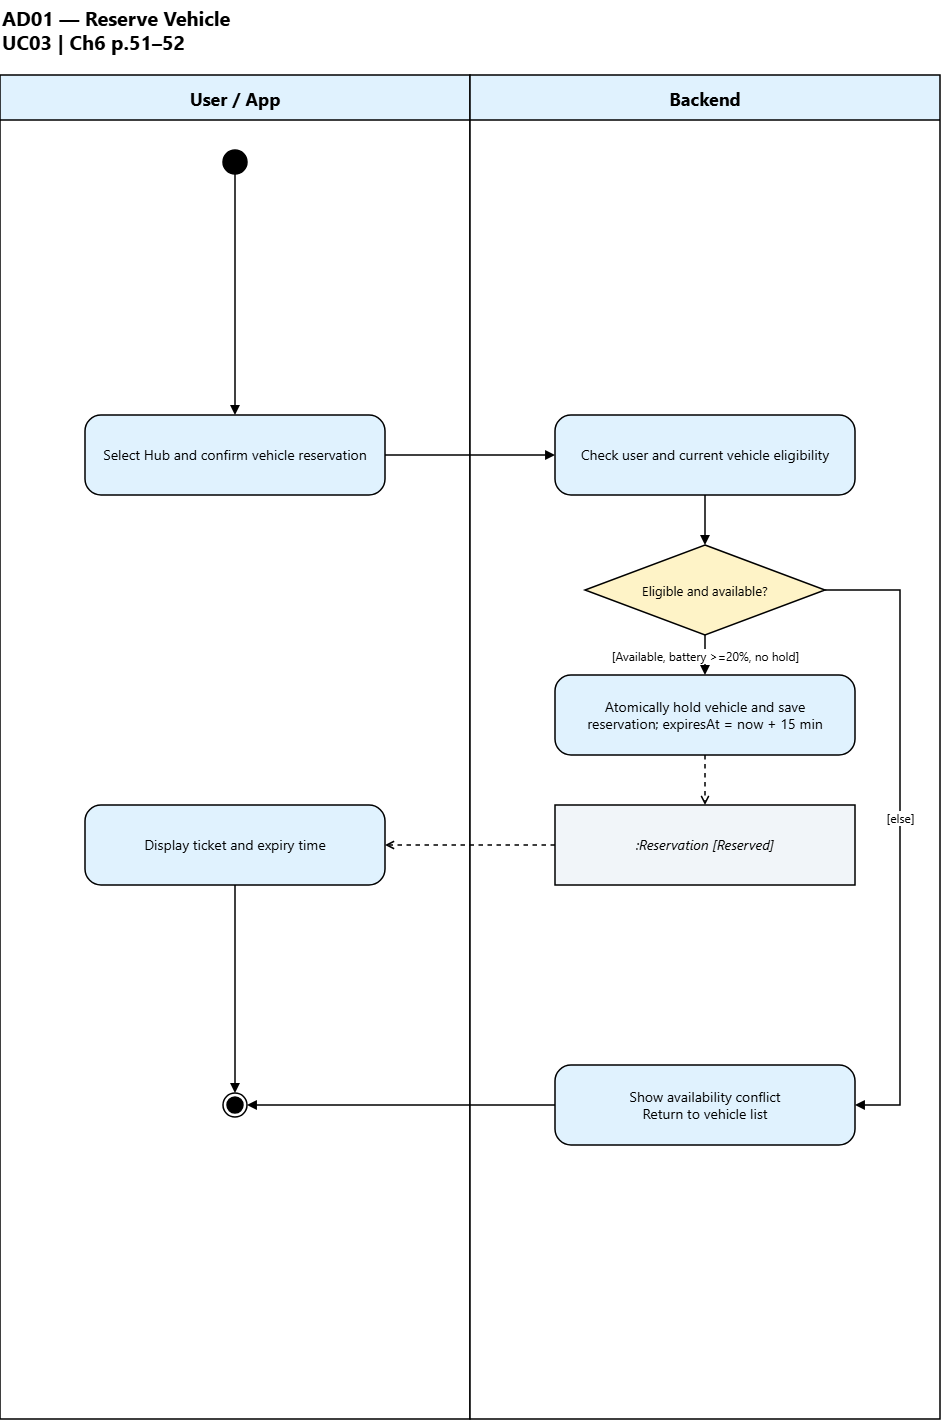
\includegraphics[width=0.95\textwidth,height=0.82\textheight,keepaspectratio]{graphics/diagrams/AD01-Reserve_Vehicle.png}
    \caption{Sơ đồ hoạt động đặt giữ xe dùng chung (\texttt{AD01 -- UC03})}
    \label{fig:ad-01}
\end{figure}

\clearpage
\begin{figure}[H]
    \centering
    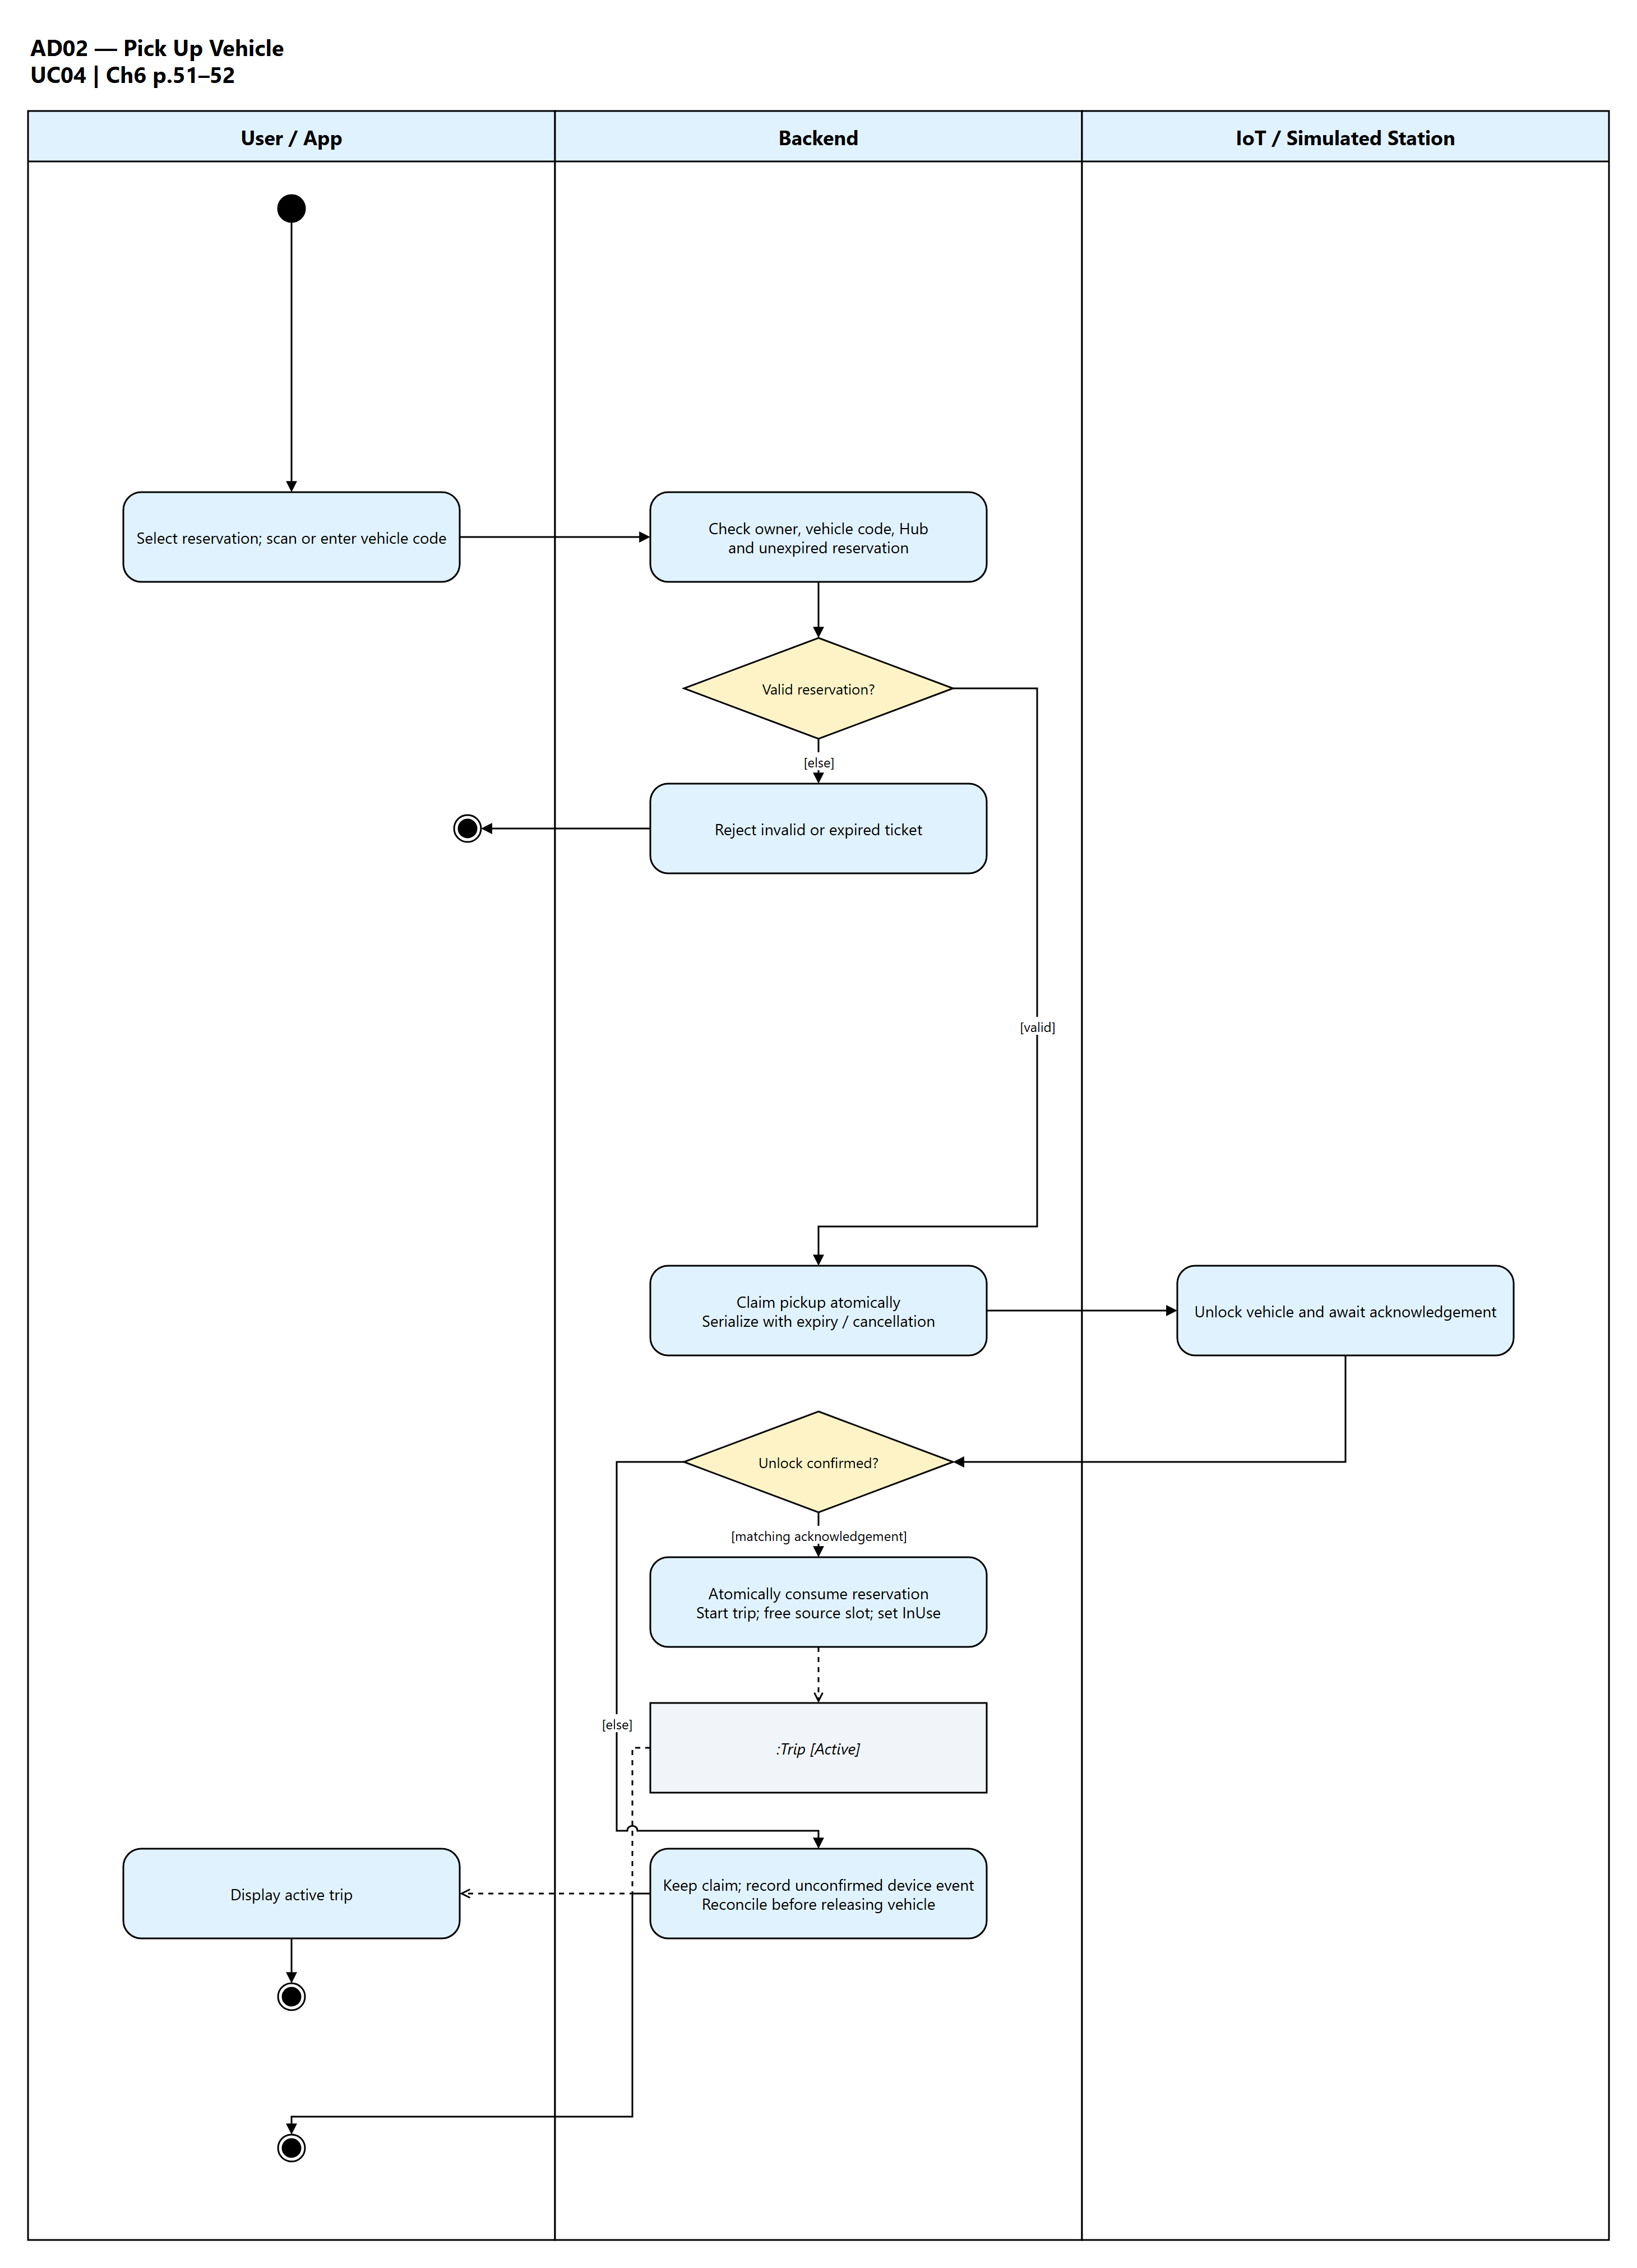
\includegraphics[width=0.95\textwidth,height=0.82\textheight,keepaspectratio]{graphics/diagrams/AD02-Pick_Up_Vehicle.png}
    \caption{Sơ đồ hoạt động nhận xe tại Hub (\texttt{AD02 -- UC04})}
    \label{fig:ad-02}
\end{figure}

\clearpage
\begin{figure}[H]
    \centering
    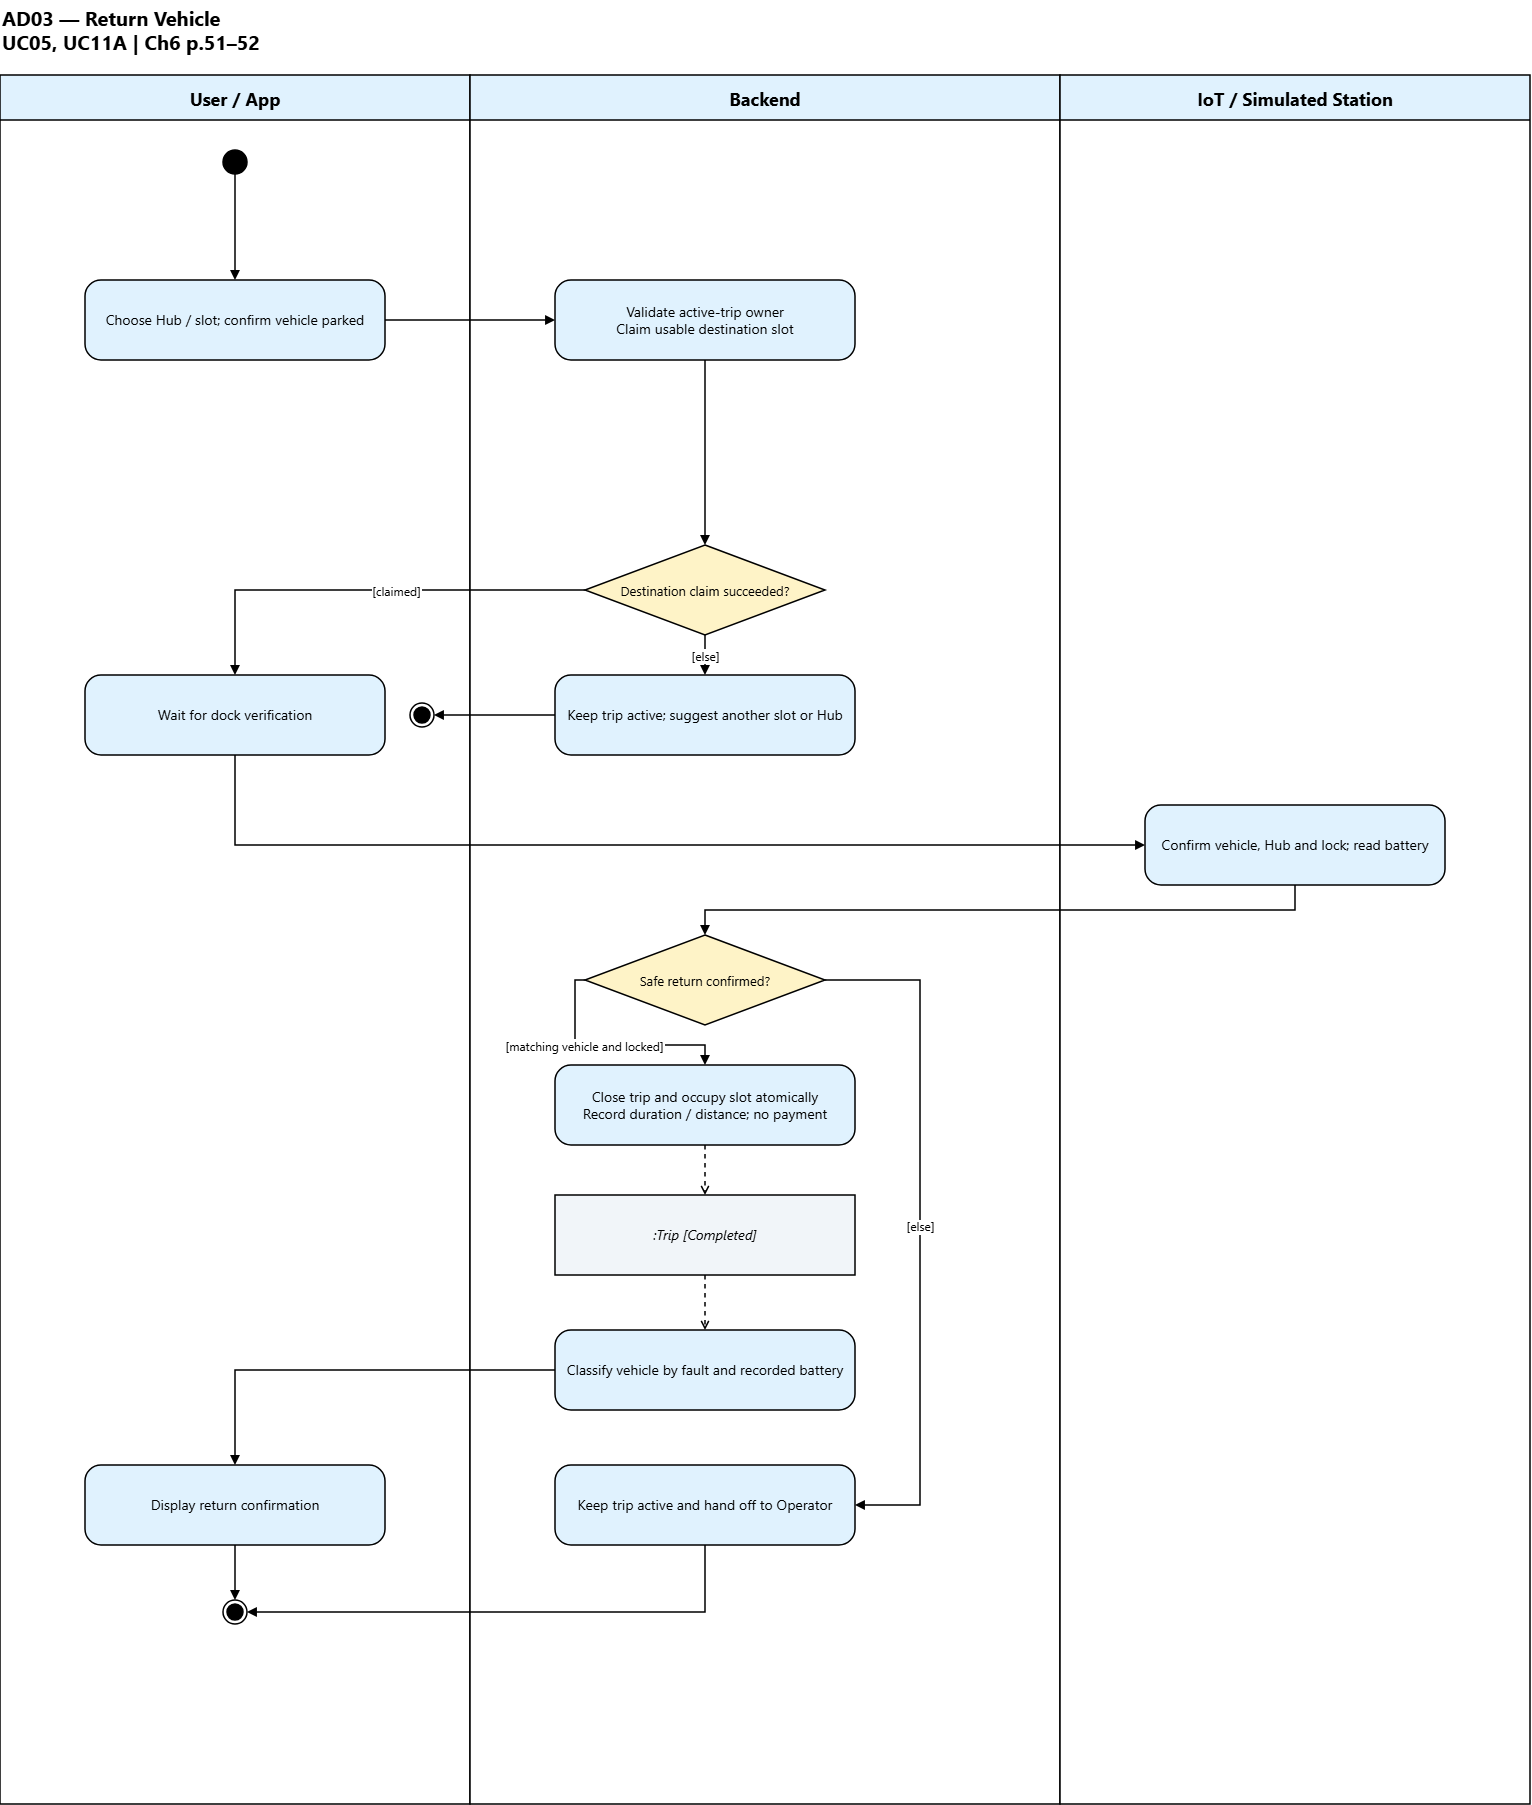
\includegraphics[width=0.95\textwidth,height=0.82\textheight,keepaspectratio]{graphics/diagrams/AD03-Return_Vehicle.png}
    \caption{Sơ đồ hoạt động trả xe tại Hub đích (\texttt{AD03 -- UC05})}
    \label{fig:ad-03}
\end{figure}

\clearpage
\begin{figure}[H]
    \centering
    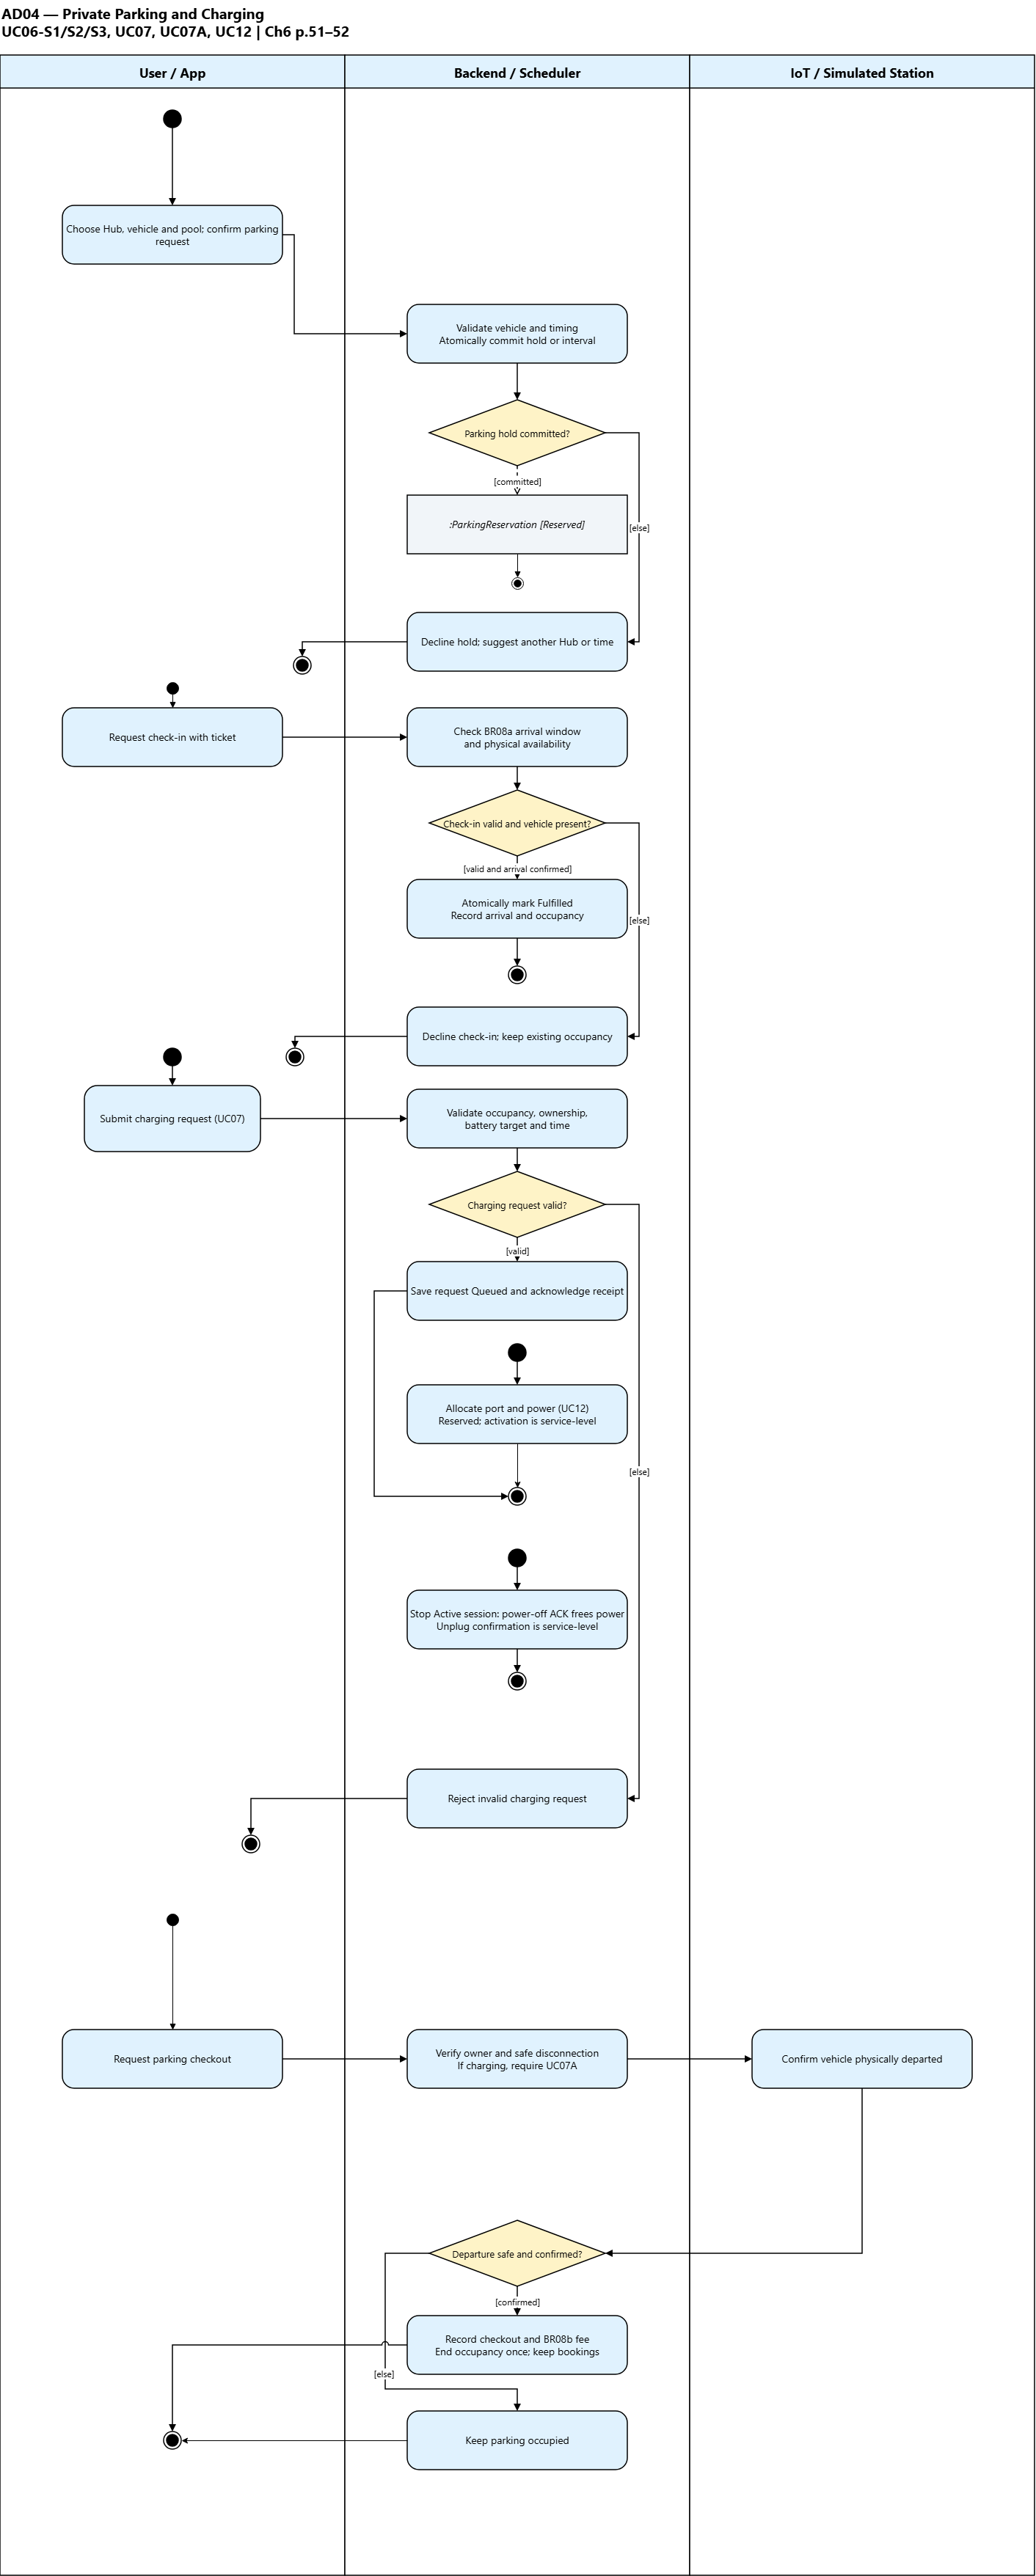
\includegraphics[width=0.95\textwidth,height=0.82\textheight,keepaspectratio]{graphics/diagrams/AD04-Reserve_Parking_and_Charging.png}
    \caption{Sơ đồ hoạt động đặt chỗ đỗ, sạc và dừng sạc xe cá nhân (\texttt{AD04 -- UC06, UC07, UC12})}
    \label{fig:ad-04}
\end{figure}

\clearpage
\begin{figure}[H]
    \centering
    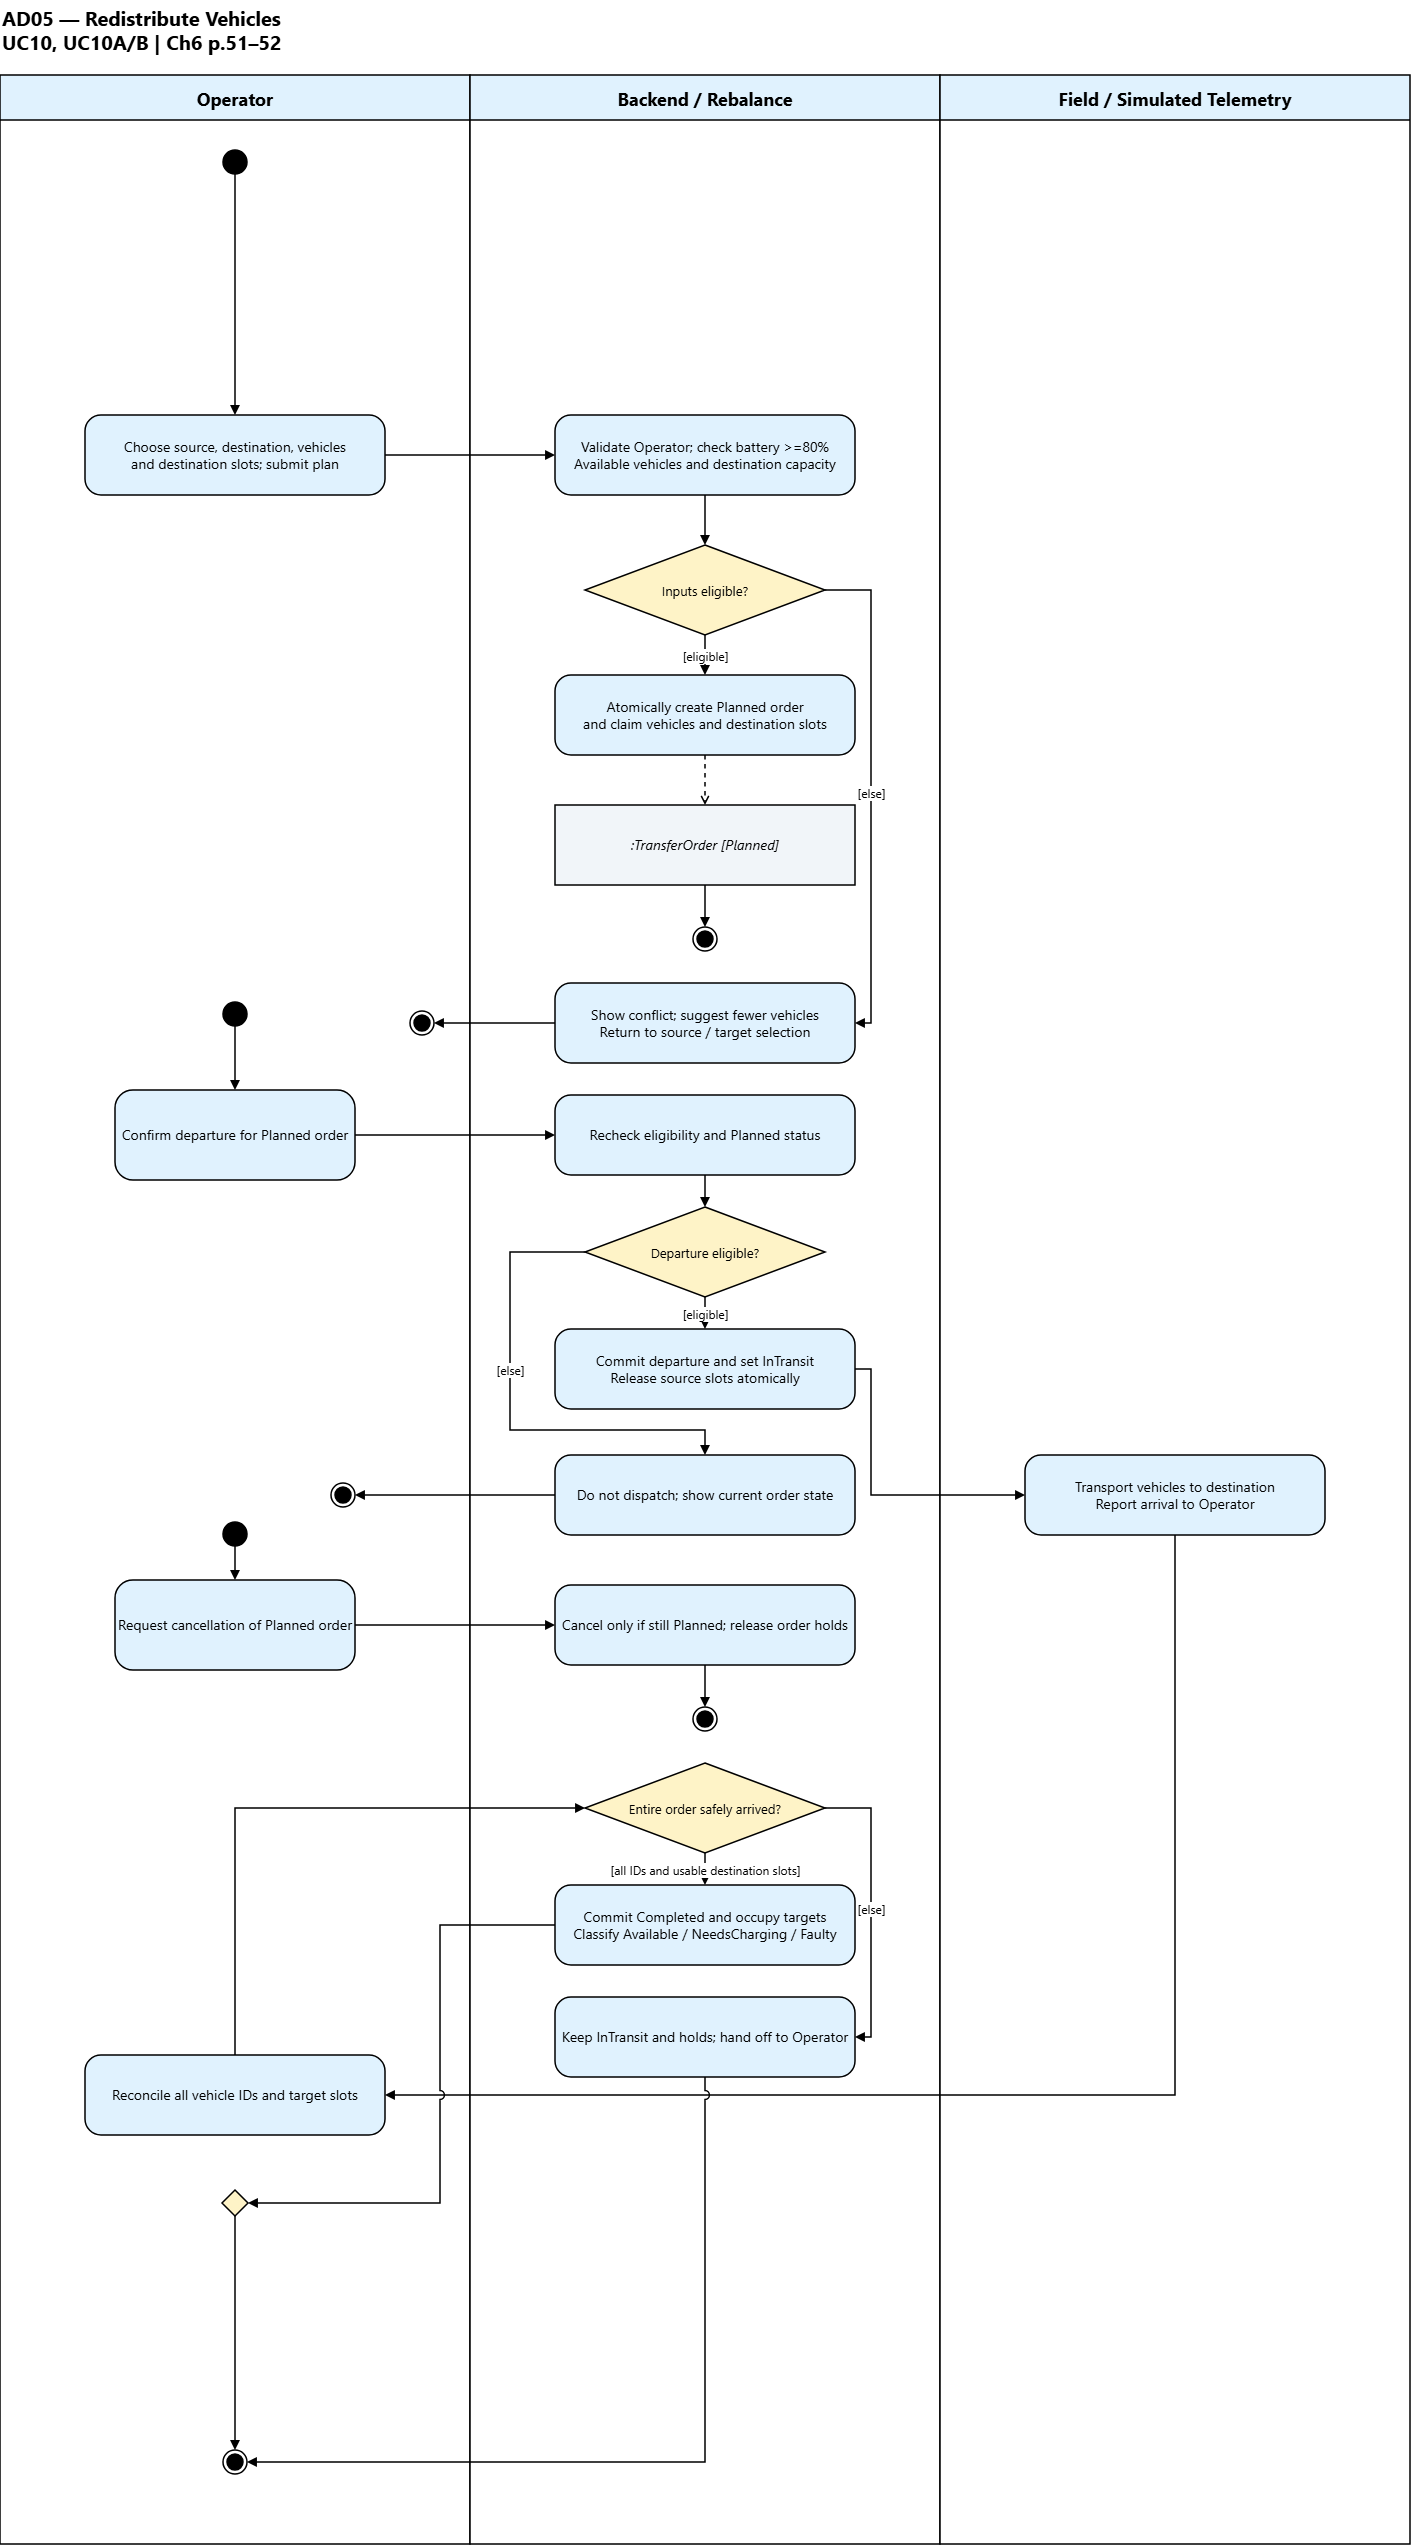
\includegraphics[width=0.95\textwidth,height=0.82\textheight,keepaspectratio]{graphics/diagrams/AD05-Redistribute_Vehicles.png}
    \caption{Sơ đồ hoạt động điều chuyển xe liên Hub (\texttt{AD05 -- UC10, UC10A/B})}
    \label{fig:ad-05}
\end{figure}

\clearpage
\begin{figure}[H]
    \centering
    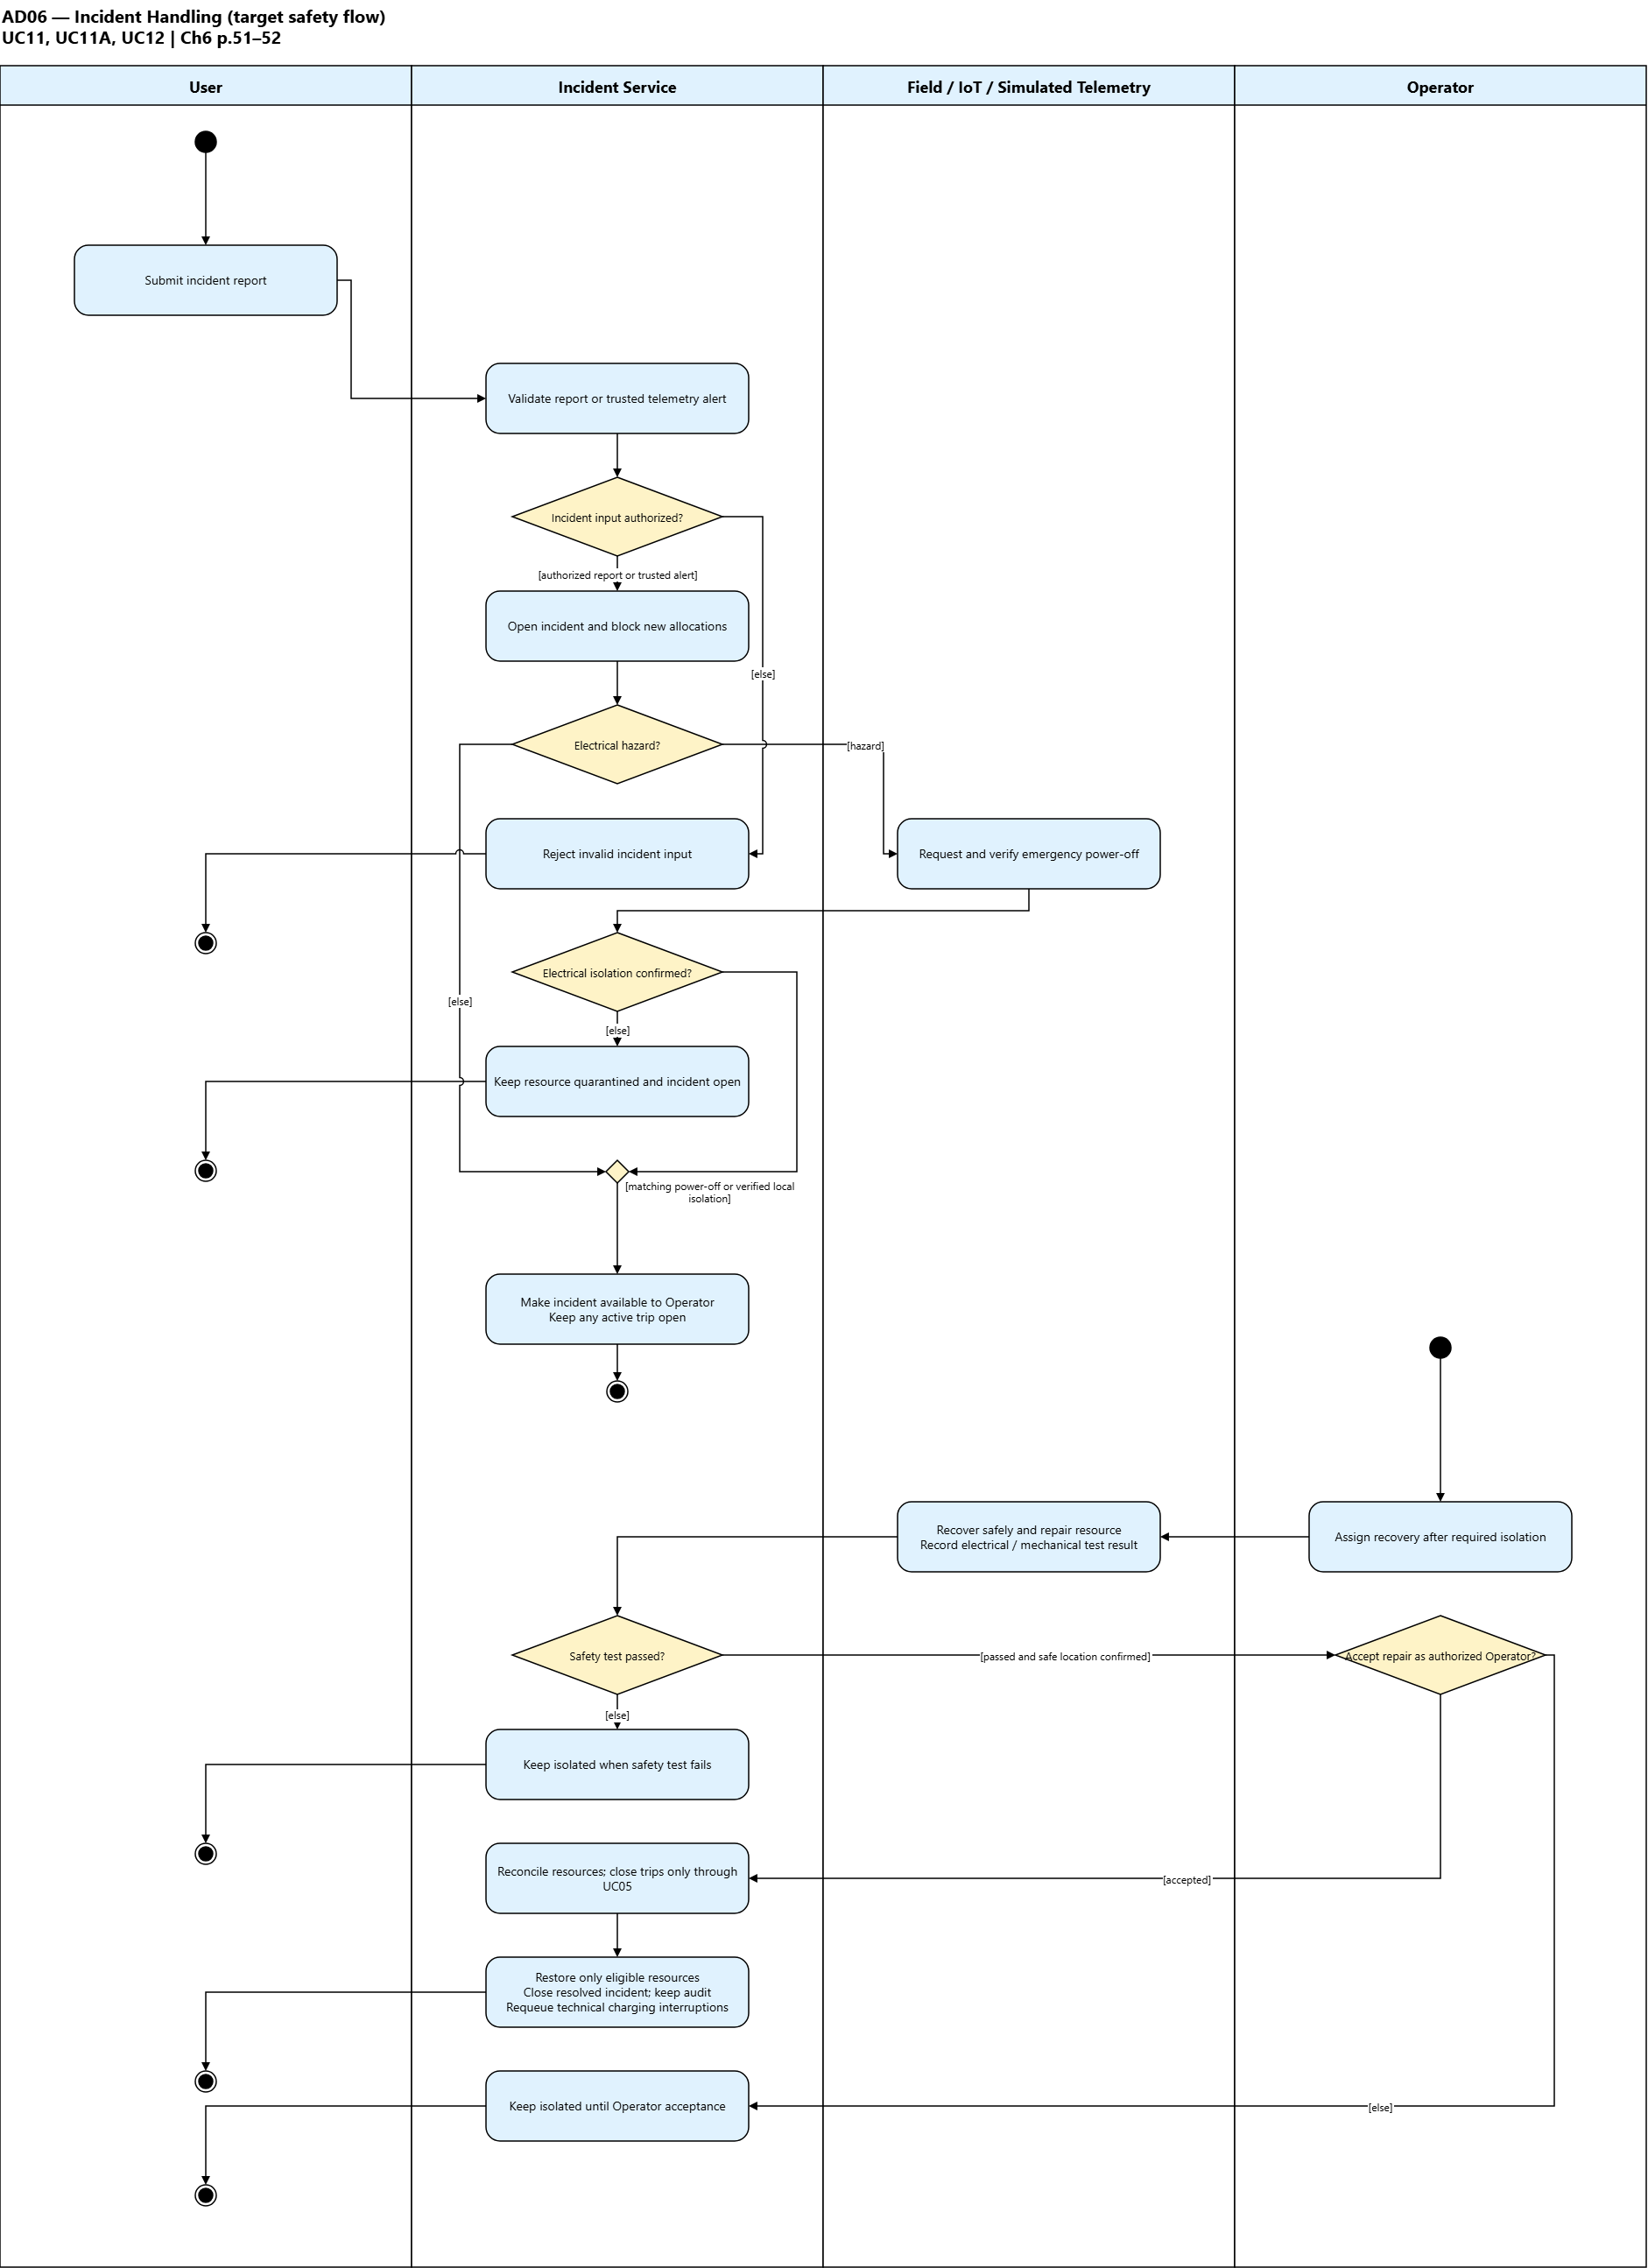
\includegraphics[width=0.95\textwidth,height=0.82\textheight,keepaspectratio]{graphics/diagrams/AD06-Handle_Operational_Incident.png}
    \caption{Sơ đồ hoạt động xử lý sự cố vận hành (\texttt{AD06 -- UC11, UC11A})}
    \label{fig:ad-06}
\end{figure}

\clearpage
\begin{figure}[H]
    \centering
    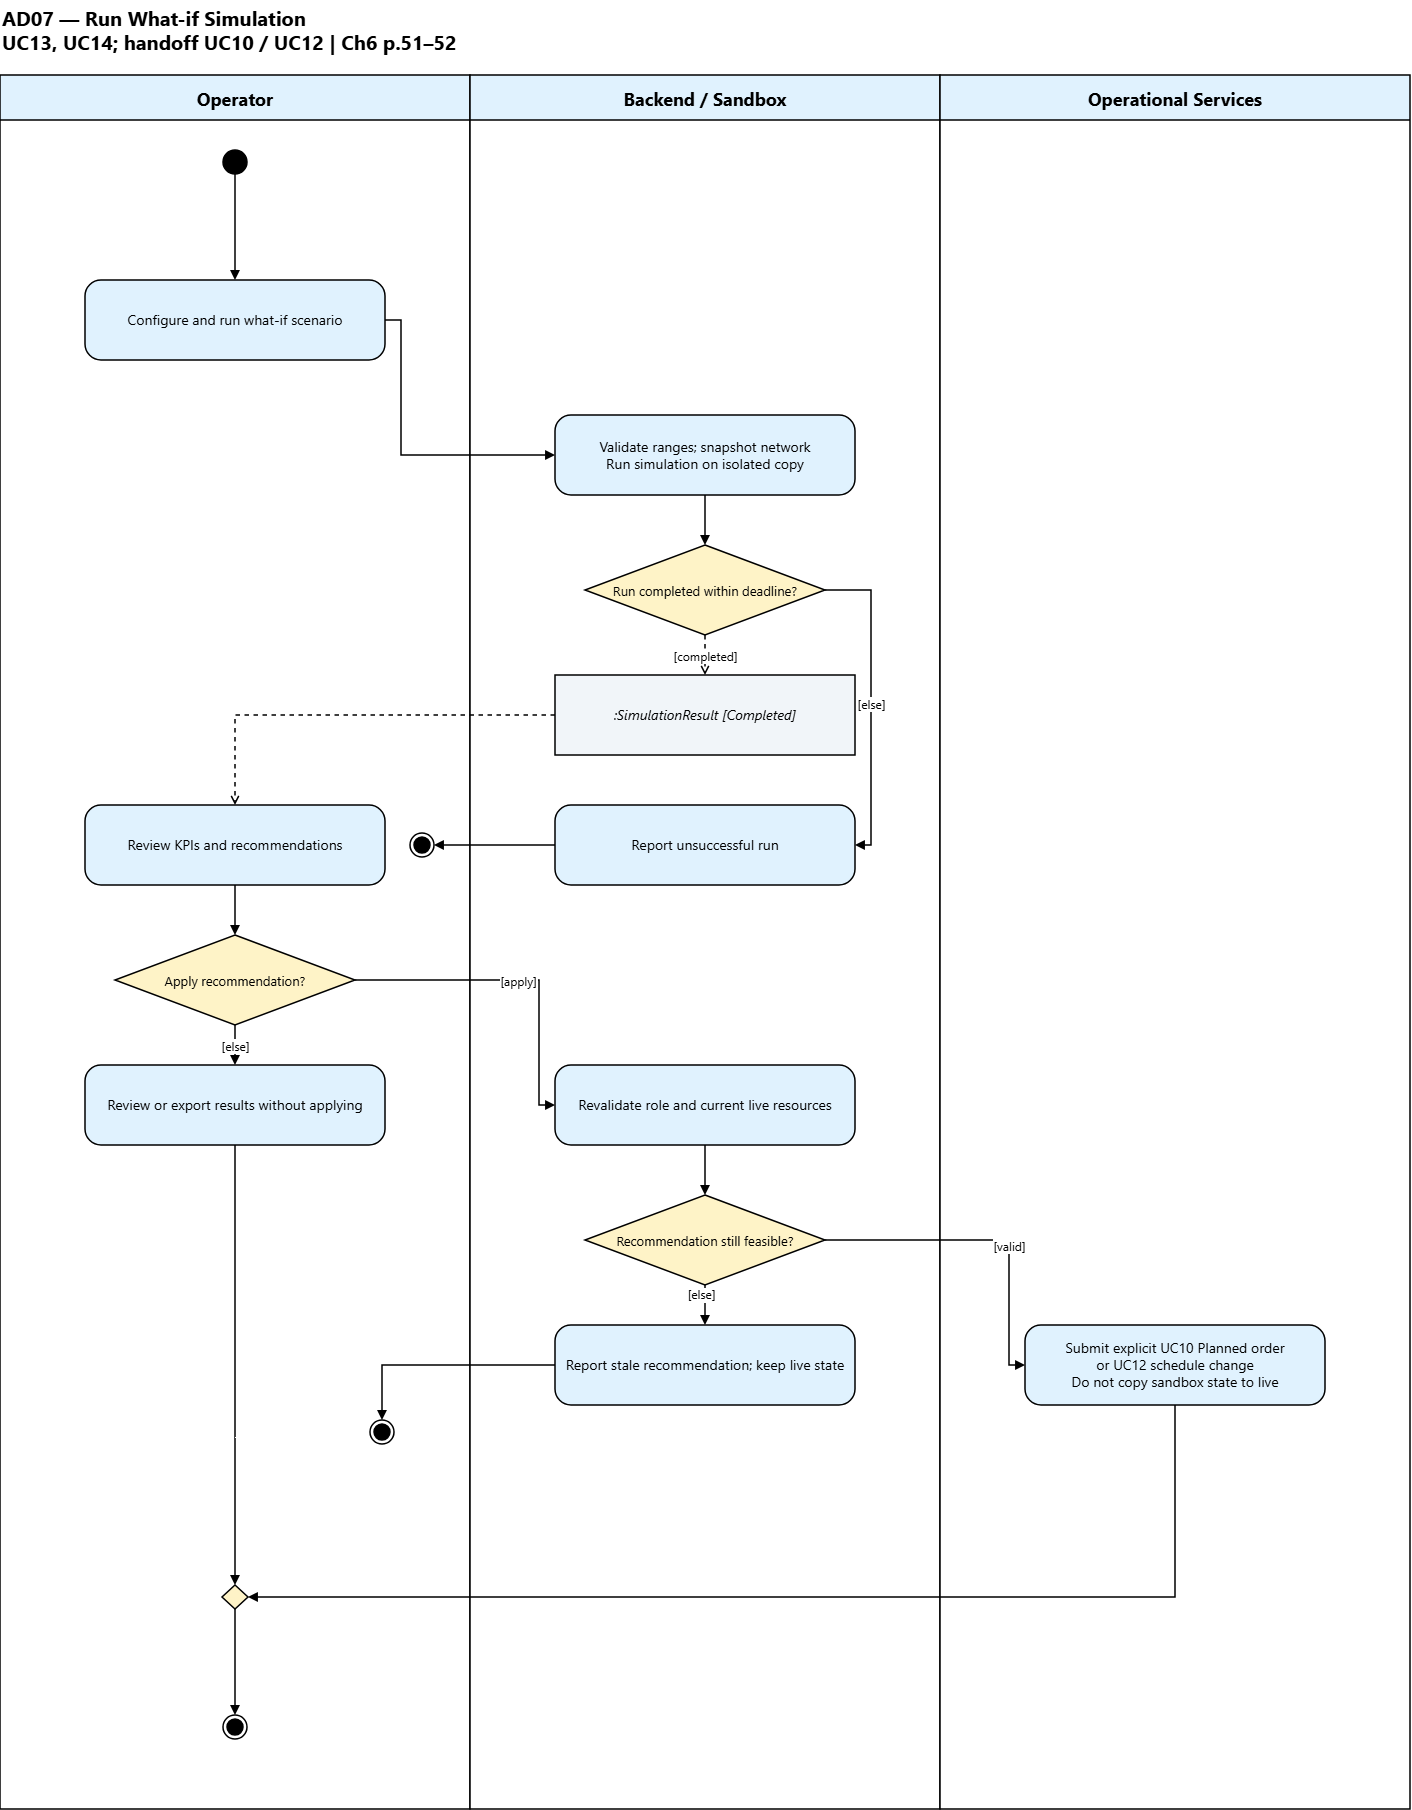
\includegraphics[width=0.95\textwidth,height=0.82\textheight,keepaspectratio]{graphics/diagrams/AD07-Run_What_if_Simulation.png}
    \caption{Sơ đồ hoạt động mô phỏng What-if (\texttt{AD07 -- UC13, UC14})}
    \label{fig:ad-07}
\end{figure}
\clearpage

\subsection{Mô hình Hành vi: Sơ đồ Trạng thái (State-chart Diagrams -- Bonus: SC01--SC03)}

Để đáp ứng tiêu chí điểm cộng của Submission \#2 và kiểm soát chuyển đổi trạng thái khi thực thi đồng thời, nhóm thiết kế 3 máy trạng thái hữu hạn cho các thực thể lõi (\Cref{fig:sc-01}--\Cref{fig:sc-03}):
\begin{enumerate}[leftmargin=*,nosep]
    \item \textbf{\texttt{SC01} -- Vòng đời Phương tiện Điện (\texttt{Vehicle State Machine}):} Mô hình hóa 10 trạng thái chuẩn (\texttt{Available}, \texttt{Reserved}, \texttt{InUse}, \texttt{Needs\allowbreak Charging}, \texttt{Charging}, \texttt{Transfer\allowbreak Held}, \texttt{InTransit}, \texttt{Faulty}, \texttt{Maintenance}, \texttt{Retired}). Điều kiện chuyển đổi phân biệt xe dùng chung (cho thuê và điều chuyển) với xe cá nhân (chỉ tham gia đỗ/sạc), đồng thời chặn chuyển về \texttt{Available} khi chưa nghiệm thu sự cố hoặc pin $< 20\%$.
    \item \textbf{\texttt{SC02} -- Vòng đời Cổng sạc (\texttt{Charging Point State Machine}):} Bao gồm 9 trạng thái (\texttt{Idle}, \texttt{Reserved}, \texttt{Starting}, \texttt{Charging}, \texttt{Stopping}, \texttt{Complete}, \texttt{Fault}, \texttt{Repair}, \texttt{Retired}), phân tách trạng thái \texttt{Complete} (đã ngắt điện, giữ đầu nối chờ rút) và duy trì khóa cô lập cổng \texttt{Fault/Repair}. Trong mã nguồn hiện tại, phần chuyển đổi từ \texttt{Reserved} sang \texttt{Active} (\texttt{activateAllocation}) và rút phích (\texttt{confirmUnplug}) được hiện thực ở tầng \texttt{ChargingService} kèm unit test, chưa mở route HTTP công khai.
    \item \textbf{\texttt{SC03} -- Vòng đời Đặt giữ và Chuyến đi (\texttt{Reservation and Trip State Machine}):} Quản lý song hành vòng đời phiếu giữ xe (\texttt{Pending}, \texttt{Reserved}, \texttt{Fulfilled}, \texttt{Cancelled}, \texttt{Expired}) với cờ \texttt{pickupClaimed} và vòng đời chuyến đi (\texttt{Active}, \texttt{Completed}). Sự cố báo giữa chuyến (\texttt{UC11A}) không tự động đóng chuyến đang \texttt{Active}.
\end{enumerate}

\clearpage
\begin{figure}[H]
    \centering
    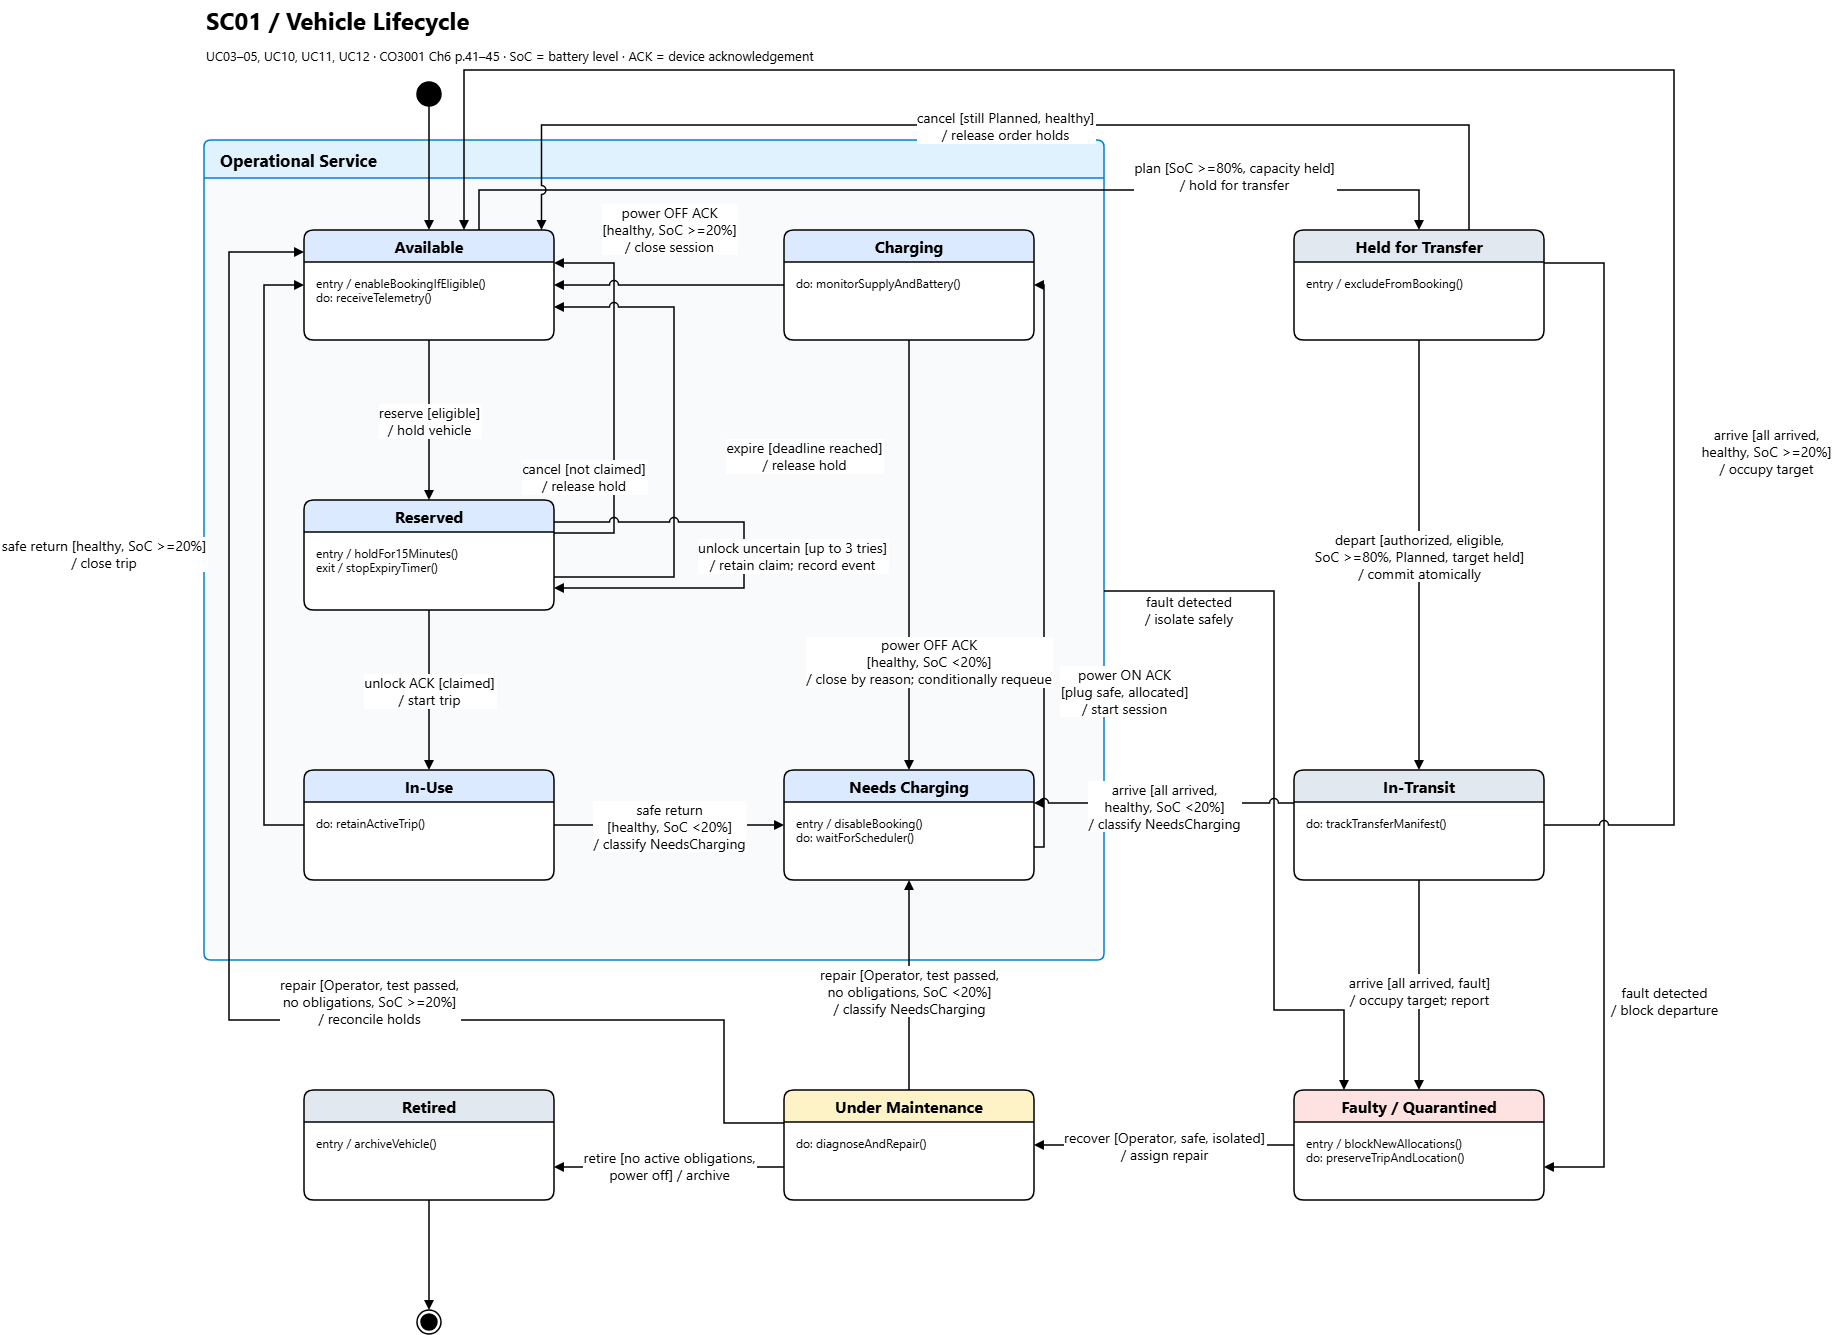
\includegraphics[width=0.95\textwidth,height=0.82\textheight,keepaspectratio]{graphics/diagrams/SC01-Vehicle_State_Machine.png}
    \caption{Sơ đồ máy trạng thái vòng đời phương tiện điện (\texttt{SC01})}
    \label{fig:sc-01}
\end{figure}

\clearpage
\begin{figure}[H]
    \centering
    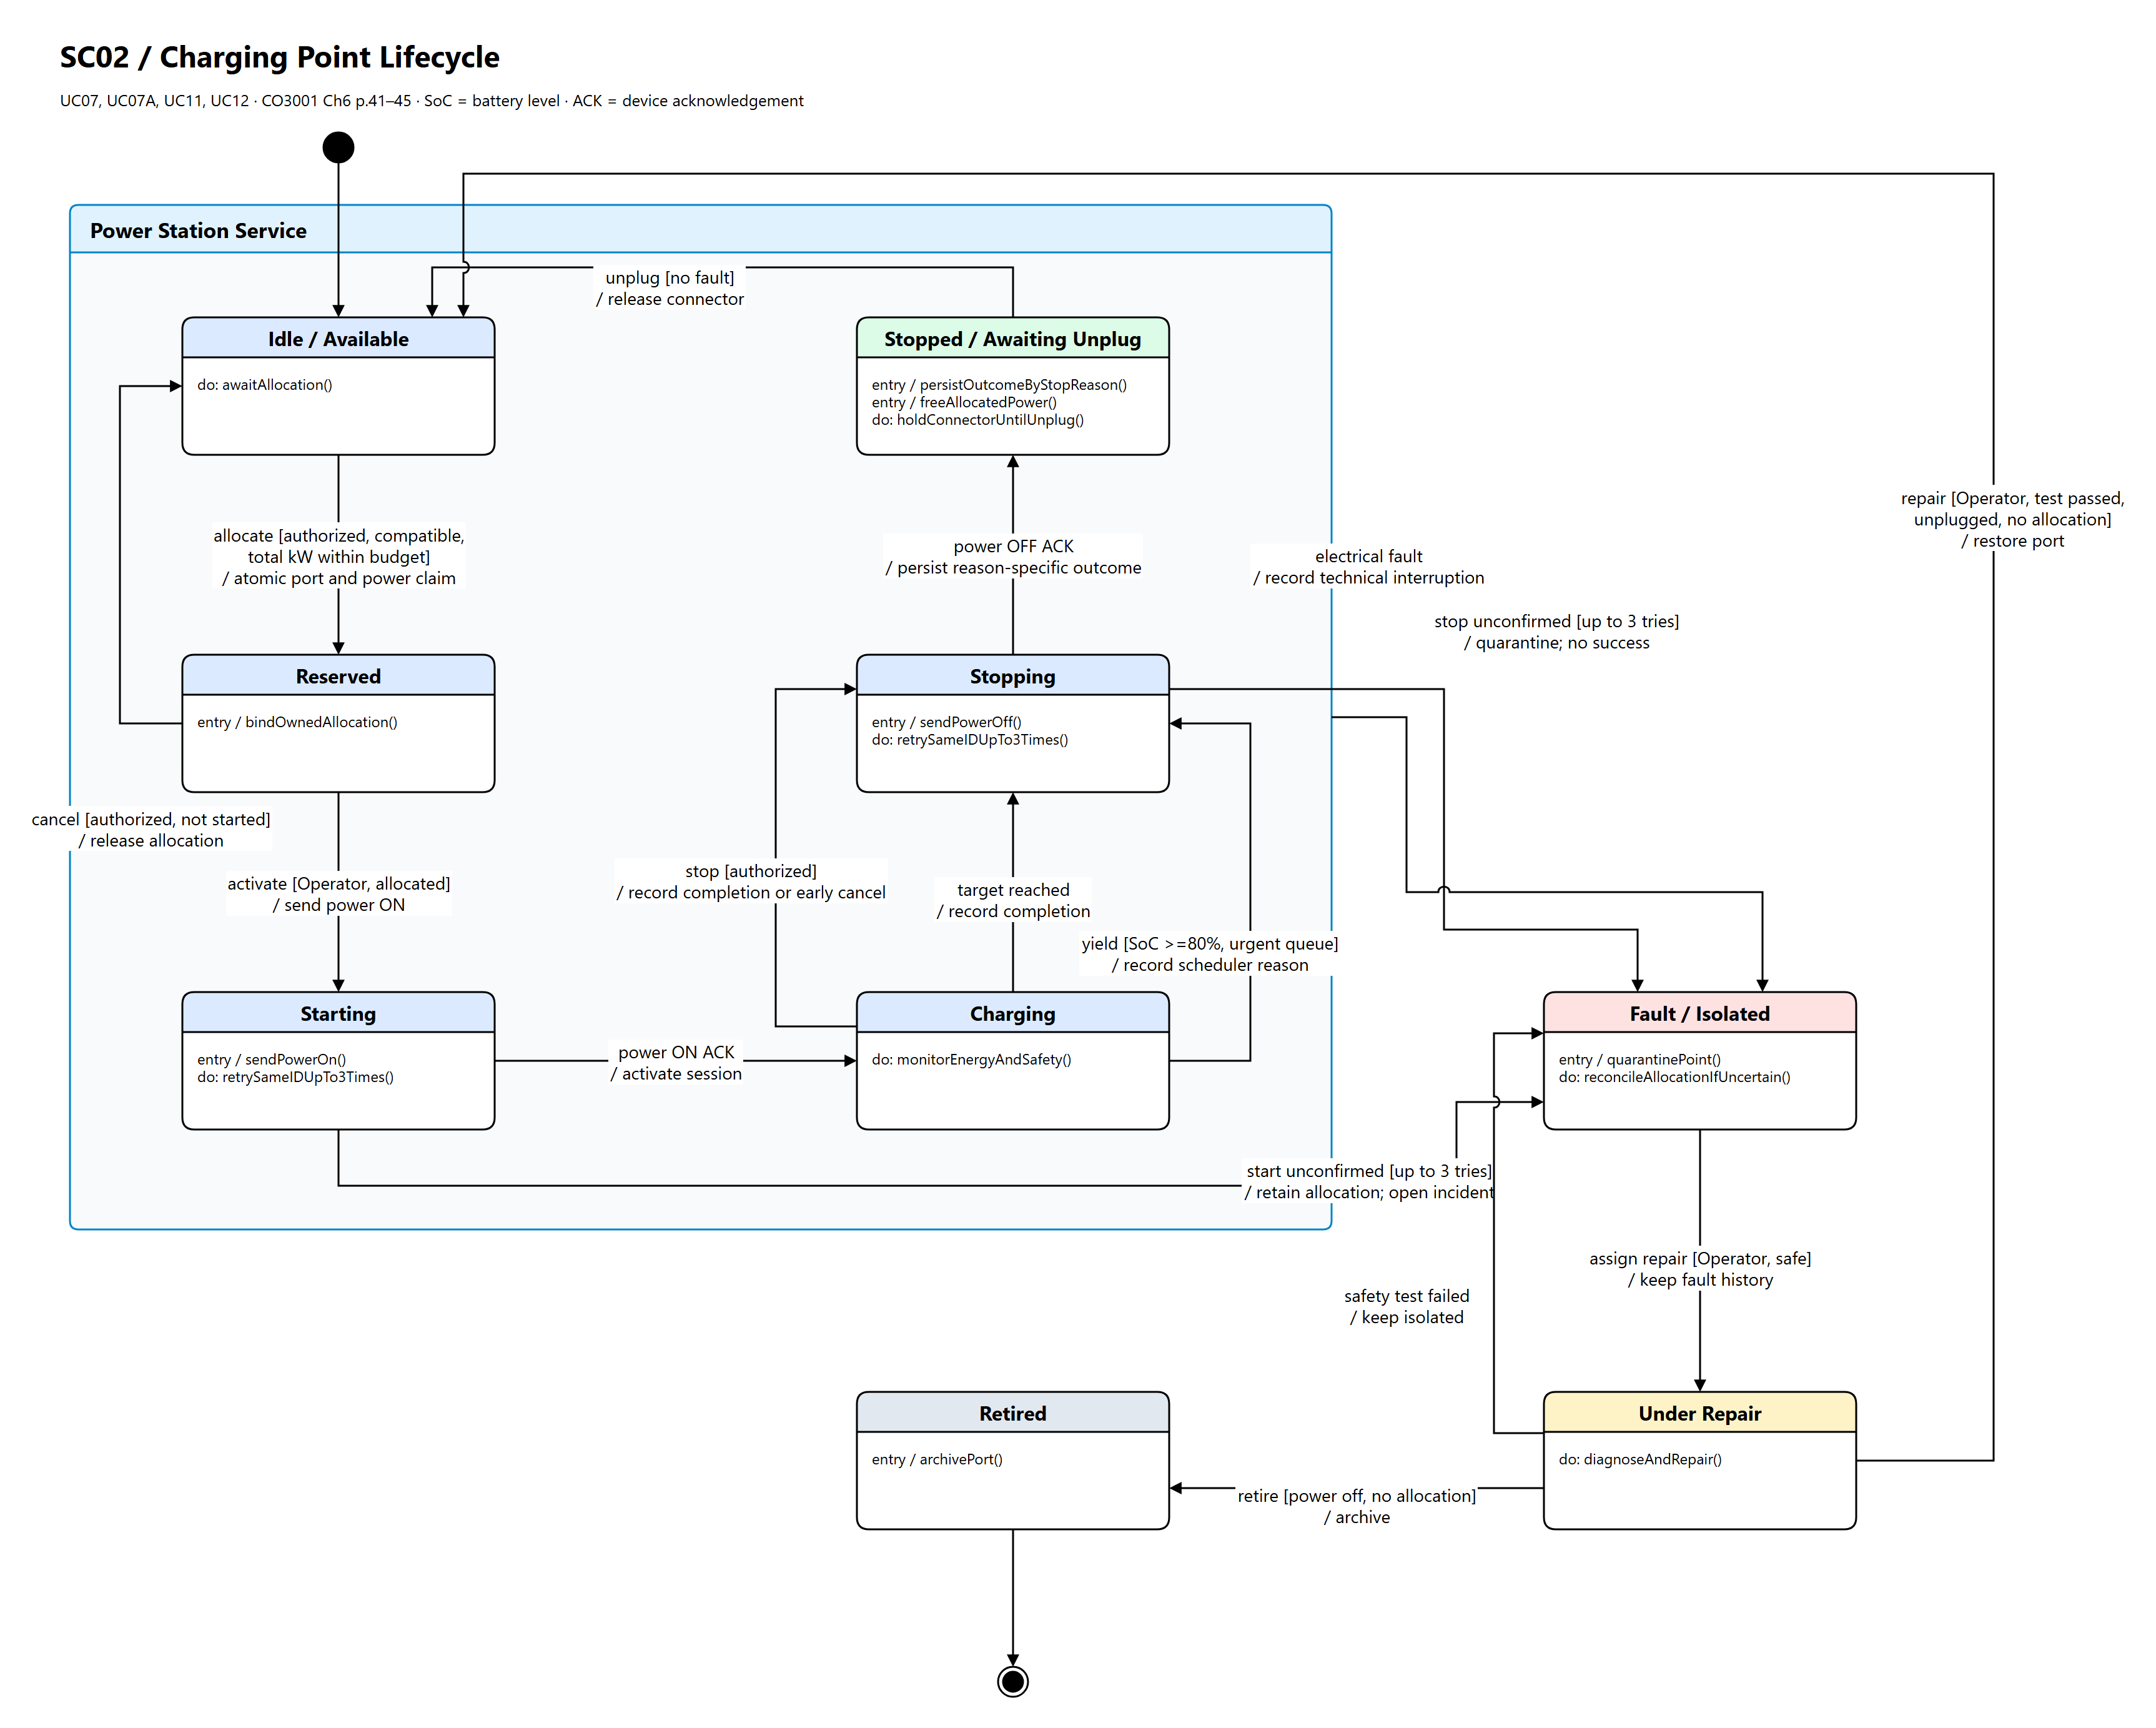
\includegraphics[width=0.95\textwidth,height=0.82\textheight,keepaspectratio]{graphics/diagrams/SC02-Charging_Point_State_Machine.png}
    \caption{Sơ đồ máy trạng thái vòng đời cổng sạc (\texttt{SC02})}
    \label{fig:sc-02}
\end{figure}

\clearpage
\begin{figure}[H]
    \centering
    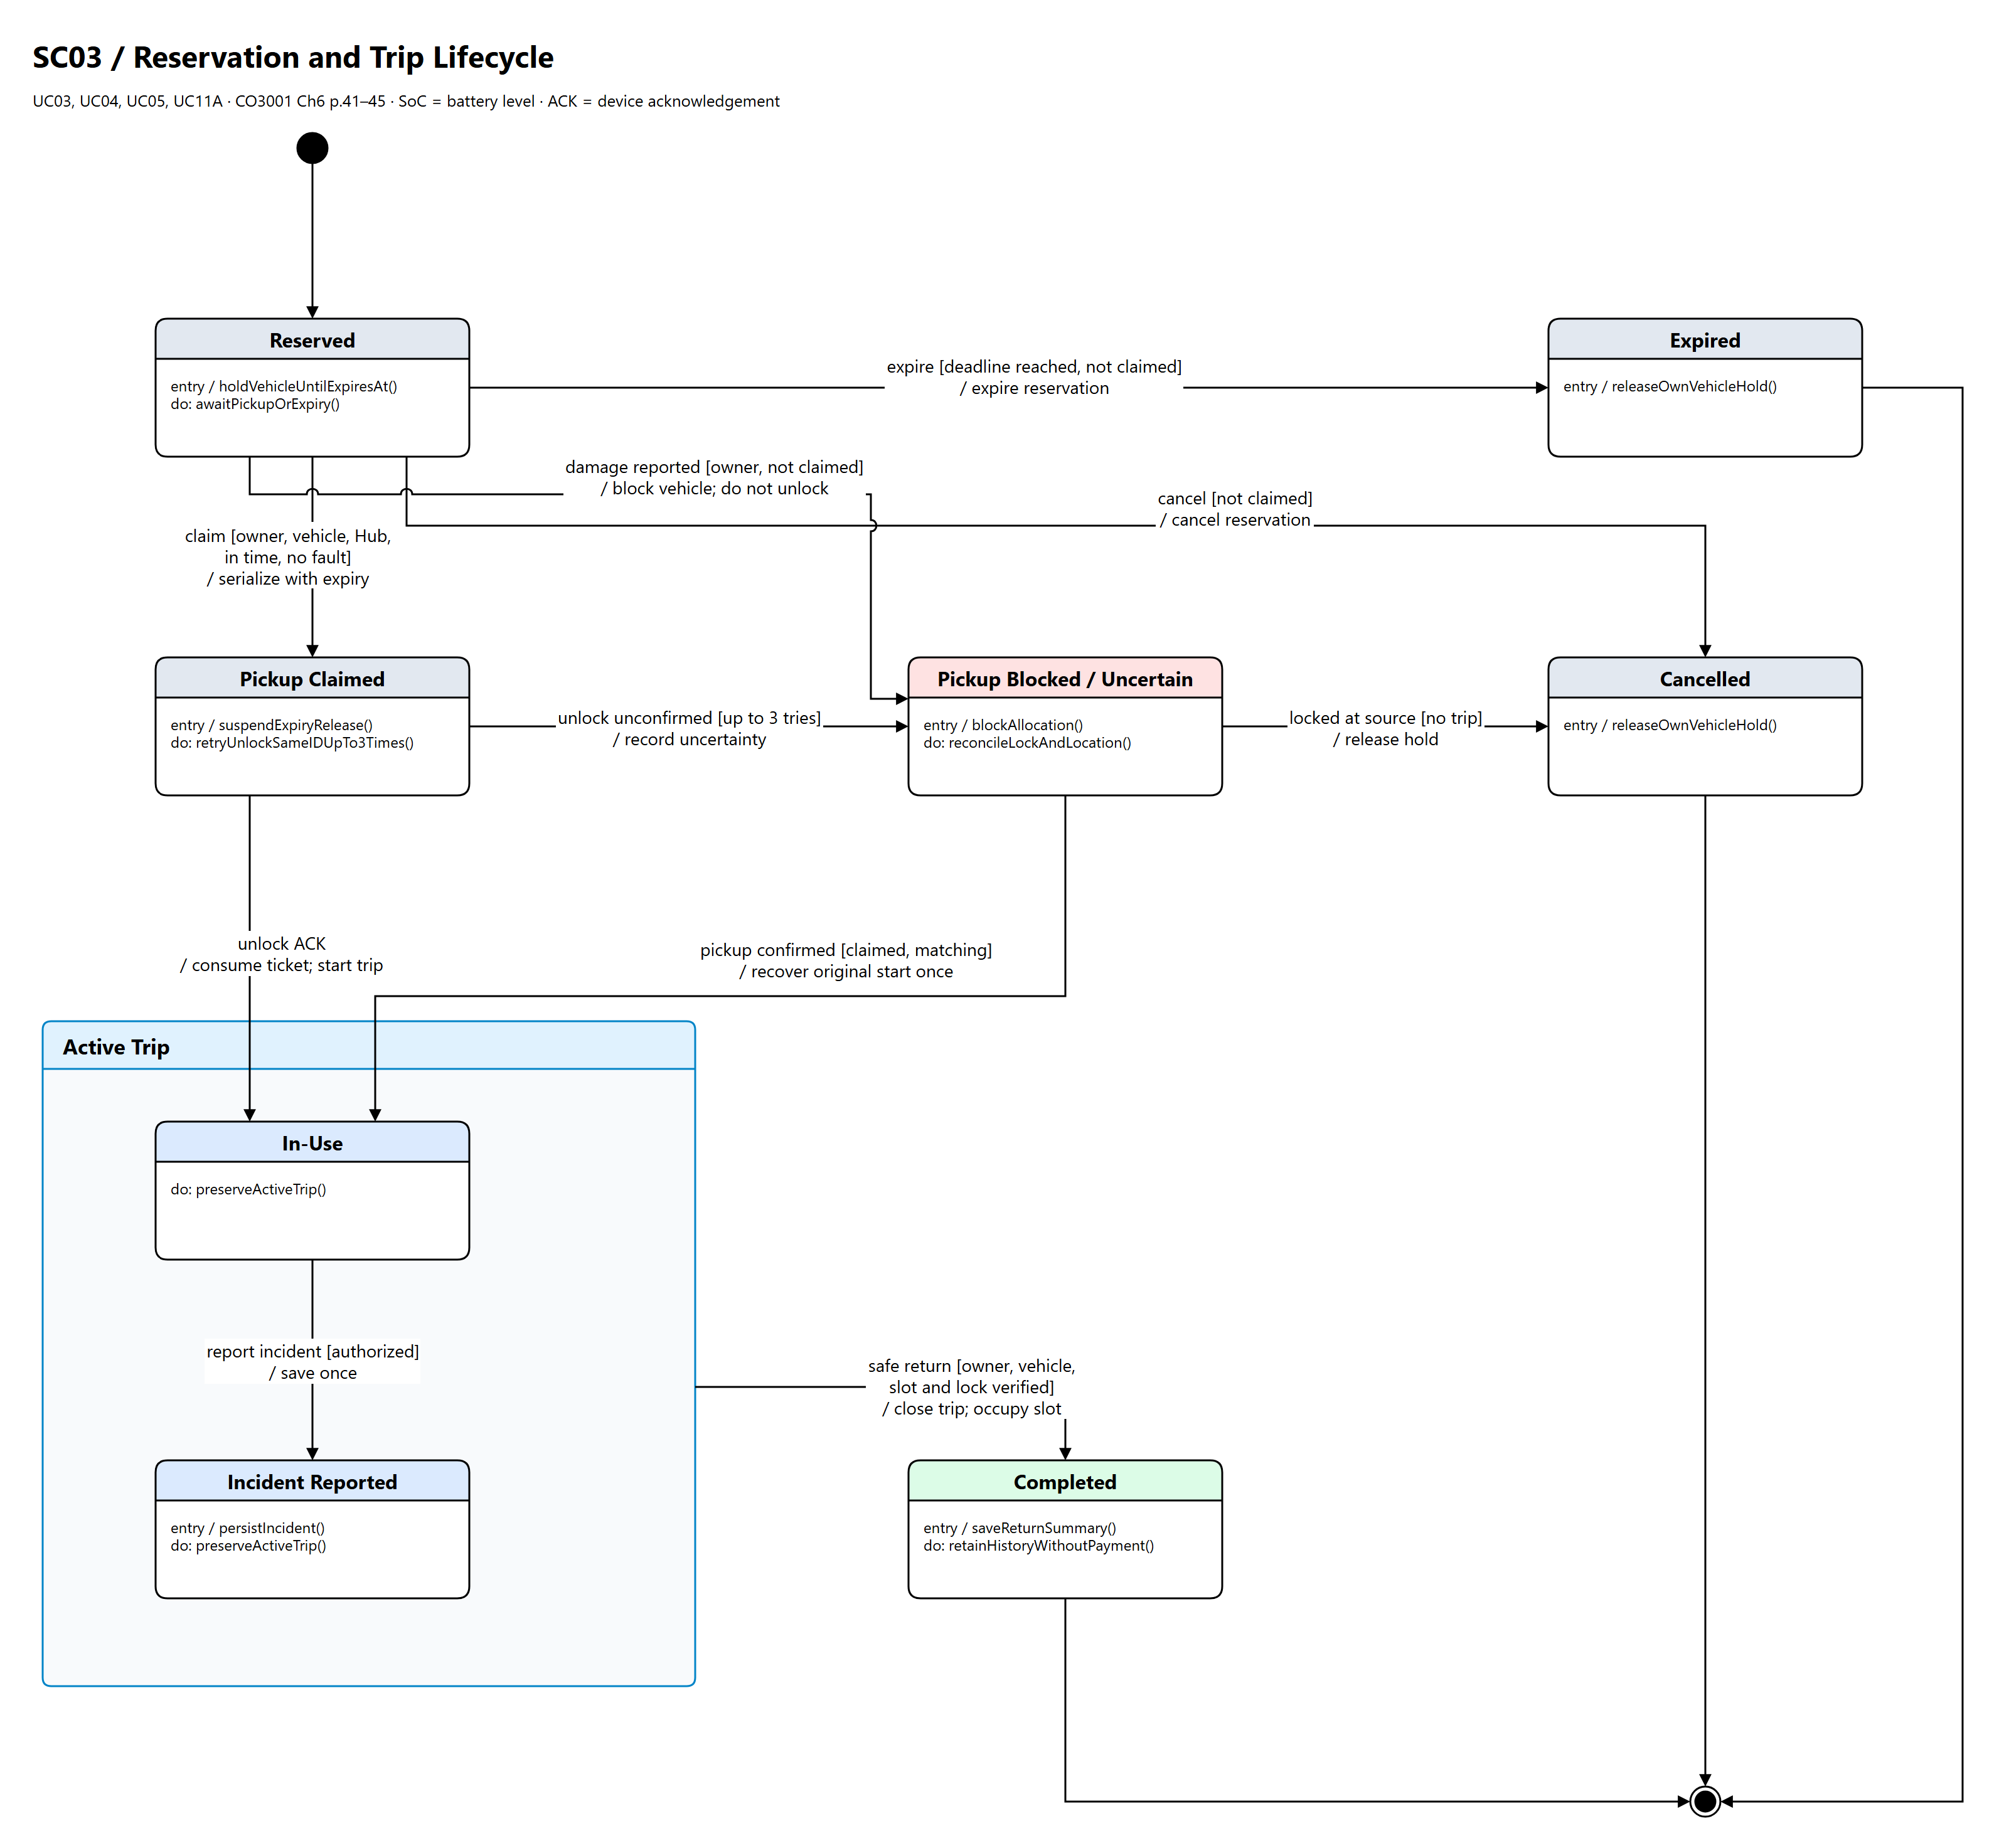
\includegraphics[width=0.95\textwidth,height=0.82\textheight,keepaspectratio]{graphics/diagrams/SC03-Reservation_and_Trip_State_Machine.png}
    \caption{Sơ đồ máy trạng thái đặt giữ và chuyến đi (\texttt{SC03})}
    \label{fig:sc-03}
\end{figure}

\clearpage

% ===================================================
% CHƯƠNG 3: KIẾN TRÚC HỆ THỐNG VÀ THIẾT KẾ CHI TIẾT (SUBMISSION #3)
% Nguồn: docs/architecture/DECISION.md, docs/reports/DEVELOPMENT_IMPLEMENTATION_VIEW_REPORT.md
% Slide tham chiếu: 07_Ch7 Architectural Design_2025.pdf (4+1 View Model), 06_Ch6 System Modeling_2025.pdf (Structural Models)
% ===================================================
\section{Kiến trúc Hệ thống và Thiết kế Chi tiết}

\subsection{Quyết định Kiến trúc và Mẫu Kiến trúc (Architectural Patterns)}
% TODO: Trích từ docs/architecture/DECISION.md
% - Áp dụng mô hình 4+1 View (Ch7); kiến trúc Modular Monolith kết hợp Layered Architecture Pattern
%   (5 tầng: Presentation -> API/Interface -> Application -> Domain -> Infrastructure) và Repository Pattern.
% - Công nghệ mục tiêu: Node.js + Express + SQLite.

\subsection{Góc nhìn Triển khai (Deployment View -- DP01)}
% TODO: Chèn và mô tả docs/diagrams/deployment/DP01-deployment.drawio
%       và docs/diagrams/deployment/README-deployment.md.

\subsection{Góc nhìn Phát triển và Hiện thực (Development View -- DV01, DV02)}
% TODO: Trích từ docs/reports/DEVELOPMENT_IMPLEMENTATION_VIEW_REPORT.md
% - Chèn DV01-Component_Diagram_New.drawio và DV02-Package_Diagram_New.drawio
% - Giải thích ranh giới tầng, Ports/Adapters (InventoryInterface, tripReader).
% - Lưu ý truy vết: DV01/DV02 phân rã 5 module logic (Accounts & Resources, Reservations & Trips,
%   Charging, Operations, Simulation); khi hiện thực MVP (Chương 4) gộp thành 3 module code theo DEVELOPMENT_GUIDE.md.

\subsection{Mô hình Cấu trúc: Sơ đồ Lớp (Class Diagram)}
% TODO: Chèn docs/diagrams/05_Class_Diagram/smart_emobility_class_diagram.drawio
%       (19 lớp thực thể/dịch vụ, 18 operations, 31 associations và bội số quan hệ).

\subsection{Đặc tả Lớp và Phương thức (Method Descriptions)}
% TODO: Tổng hợp hợp đồng tiền điều kiện, hậu điều kiện, tham số, giá trị trả về và ngoại lệ
%       cho 100% phương thức từ .agent/class-diagram/CLASS_CATALOG.md.

\subsection{Thiết kế Cơ sở dữ liệu (SQLite Schema và Migrations)}
% TODO: Trình bày 12 migrations (app/db/migrations/0001..0012), chế độ WAL và transaction BEGIN IMMEDIATE.

\clearpage

% ===================================================
% CHƯƠNG 4: HIỆN THỰC MVP, KIỂM THỬ VÀ TRÌNH DIỄN HỆ THỐNG
% Nguồn: app/src/, docs/audits/post-merge/, docs/architecture/MINH_DEMO_GUIDE.md
% Slide tham chiếu: 08_Ch8 Implementation_2025.pdf, 09_Ch9 Software Testing_2025.pdf
% ===================================================
\section{Hiện thực MVP, Kiểm thử và Trình diễn Hệ thống}

\subsection{Cấu trúc 3 Module Backend và Tích hợp}
% TODO: Mô tả 3 module thực tế trong app/src/modules/ (ánh xạ từ 5 module thiết kế ở Chương 3):
% 1. mobility-simulation (UC01-05, UC13-14)
% 2. parking-charging (UC06, UC07, UC12 -- bổ sung ở PR #16 với Migration 0012)
% 3. operations (UC08-11, InventoryInterface) -- tham khảo docs/architecture/operations-architecture.html.

\subsection{Kiểm thử Phần mềm và Kịch bản Kiểm thử (Test Cases -- Bonus)}
% TODO: Phân tầng theo Ch9 (Unit / Component / System & Integration testing)
%       Tổng hợp cả 31 file kiểm thử (183 test cases) trong app/src/:
%       - Core (5 file, 10 tests), Mobility-Simulation (8 file, 27 tests),
%       - Operations (12 file, 121 tests), Parking-Charging (6 file, 25 tests).
%       (Lưu ý: Báo cáo audit docs/audits/post-merge/EXECUTIVE_SUMMARY.md ghi 144/144 pass tại commit ac21515 trước PR #16;
%        khi chạy báo cáo cuối kỳ cần chạy lại `npm test --prefix app` sau khi cài dependencies để lấy số pass mới nhất).

\subsection{Trình diễn Sản phẩm Mẫu (Working Demonstration)}
% TODO: Bắt buộc theo PDF trang 5 ("A working demonstration by sequence of screens"):
% - Chuỗi màn hình Live Web App (app/prototype/live.html, app/src/demo-server.js, MINH_DEMO_GUIDE.md)
% - Chuỗi màn hình Prototype Mockup (app/prototype/index.html, gallery.html)
% - Nêu minh bạch ranh giới giữa luồng đã nối Live UI và luồng kiểm chứng qua Backend API + Test Suite.

\clearpage

% ===================================================
% CHƯƠNG 5: ĐÁNH GIÁ, BÀI HỌC KINH NGHIỆM VÀ HƯỚNG PHÁT TRIỂN
% Nguồn: docs/audits/post-merge/REMEDIATION_ROADMAP.md, 04_BTL_SoftwareEngineering_HK261.pdf (trang 4)
% ===================================================
\section{Đánh giá, Bài học Kinh nghiệm và Hướng Phát triển}

\subsection{Đánh giá Kết quả Đạt được}
% TODO: So sánh với yêu cầu tối thiểu của đề bài (SQLite ACID + 12 migrations, 31 test files / 183 test cases trên 3 modules, Playwright UI check).

\subsection{Hạn chế Hiện tại và Hướng Phát triển}
% TODO: Trích từ docs/audits/post-merge/REMEDIATION_ROADMAP.md
% - Hoàn thiện nối Live UI cho UC08/09/11 và Parking/Charging; tích hợp thiết bị IoT thực tế (OCPP/MQTT).

\subsection{Bài học Kinh nghiệm của Nhóm (Lessons Learned)}
% TODO: Tổng hợp bài học về quản lý trạng thái, kiểm soát đồng thời, hợp đồng API và phối hợp nhóm.

\clearpage

% ===================================================
% CHƯƠNG 6: KHAI BÁO GENERATIVE AI VÀ QUẢN TRỊ NHÓM (BẮT BUỘC)
% Nguồn: docs/references/04_BTL_SoftwareEngineering_HK261.pdf (trang 4-6), PROJECT_SPECIFICATION.md (§7-8)
% ===================================================
\section{Khai báo Minh bạch Generative AI và Quản trị Nhóm}

\subsection{Khai báo Sử dụng Generative AI (Tools, Scope, and Level of Contribution)}
% TODO: Bắt buộc theo PDF trang 5-6:
% - Bảng liệt kê Tools, Scope, Level of Contribution (mẫu tại PROJECT_SPECIFICATION.md §8)
% - Mô tả cụ thể phần nhóm tự phân tích, chỉnh sửa lỗi, viết test kiểm chứng và đóng góp nguyên bản.

\subsection{Tổ chức Họp nhóm, Biên bản Họp và Đánh giá Đóng góp}
% TODO: Tóm tắt lịch họp hằng tuần, biên bản họp theo dõi tiến độ và đánh giá đóng góp cá nhân/nhóm (Teamwork, Meeting Minutes & Peer Evaluation theo PDF trang 4).


% Tài liệu tham khảo (nếu dùng BibTeX)
% \bibliographystyle{plain}
% \bibliography{refs/example}

\end{document}
